% !TeX encoding = UTF-8
% !TeX program = xelatex
% !TeX spellcheck = en_US

\documentclass[degree=master]{thuthesis}
  % 学位 degree:
  %   doctor | master | bachelor | postdoc
  % 学位类型 degree-type:
  %   academic(默认)| professional


% 论文基本配置,加载宏包等全局配置
% !TeX root = ./thuthesis-example.tex

% 论文基本信息配置

\thusetup{
  %******************************
  % 注意:
  %   1. 配置里面不要出现空行
  %   2. 不需要的配置信息可以删除
  %   3. 建议先阅读文档中所有关于选项的说明
  %******************************
  %
  % 输出格式
  %   选择打印版(print)或用于提交的电子版(electronic),前者会插入空白页以便直接双面打印
  %
  output = electronic,
  %
  % 标题
  %   可使用“\\”命令手动控制换行
  %
  title  = {清华大学学位论文 \LaTeX{} 模板\\使用示例文档 v\version},
  title* = {An Introduction to \LaTeX{} Thesis Template of Tsinghua
            University v\version},
  %
  % 学位
  %   1. 学术型
  %      - 中文
  %        需注明所属的学科门类,例如:
  %        哲学、经济学、法学、教育学、文学、历史学、理学、工学、农学、医学、
  %        军事学、管理学、艺术学
  %      - 英文
  %        博士:Doctor of Philosophy
  %        硕士:
  %          哲学、文学、历史学、法学、教育学、艺术学门类,公共管理学科
  %          填写“Master of Arts“,其它填写“Master of Science”
  %   2. 专业型
  %      直接填写专业学位的名称,例如:
  %      教育博士、工程硕士等
  %      Doctor of Education, Master of Engineering
  %   3. 本科生不需要填写
  %
  degree-name  = {工学硕士},
  degree-name* = {Master of Science},
  %
  % 培养单位
  %   填写所属院系的全名
  %
  department = {计算机科学与技术系},
  %
  % 学科
  %   1. 学术型学位
  %      获得一级学科授权的学科填写一级学科名称,其他填写二级学科名称
  %   2. 工程硕士
  %      工程领域名称
  %   3. 其他专业型学位
  %      不填写此项
  %   4. 本科生填写专业名称,第二学位论文需标注“(第二学位)”
  %
  discipline  = {计算机科学与技术},
  discipline* = {Computer Science and Technology},
  %
  % 姓名
  %
  author  = {薛瑞尼},
  author* = {Xue Ruini},
  %
  % 指导教师
  %   中文姓名和职称之间以英文逗号“,”分开,下同
  %
  supervisor  = {郑纬民, 教授},
  supervisor* = {Professor Zheng Weimin},
  %
  % 副指导教师
  %
  associate-supervisor  = {陈文光, 教授},
  associate-supervisor* = {Professor Chen Wenguang},
  %
  % 联合指导教师
  %
  % joint-supervisor  = {某某某, 教授},
  % joint-supervisor* = {Professor Mou Moumou},
  %
  % 日期
  %   使用 ISO 格式;默认为当前时间
  %
  % date = {2019-07-07},
  %
  % 是否在中文封面后的空白页生成书脊(默认 false)
  %
  include-spine = false,
  % 参考文献
  cite-style = inline,
  %
  % 密级和年限
  %   秘密, 机密, 绝密
  %
  % secret-level = {秘密},
  % secret-year  = {10},
  %
  % 博士后专有部分
  %
  % clc                = {分类号},
  % udc                = {UDC},
  % id                 = {编号},
  % discipline-level-1 = {计算机科学与技术},  % 流动站(一级学科)名称
  % discipline-level-2 = {系统结构},          % 专业(二级学科)名称
  % start-date         = {2011-07-01},        % 研究工作起始时间
}

% 载入所需的宏包

% 可以使用 nomencl 生成符号和缩略语说明
% \usepackage{nomencl}
% \makenomenclature

% 表格加脚注
\usepackage{threeparttable}

% 表格中支持跨行
\usepackage{multirow}

% 固定宽度的表格。放在 hyperref 之前的话,tabularx 里的 footnote 显示不出来。
% \usepackage{tabularx}

% 跨页表格
% \usepackage{longtable}

% 量和单位
\usepackage{siunitx}

% 定理类环境宏包
\usepackage{amsthm}
% 也可以使用 ntheorem
% \usepackage[amsmath,thmmarks,hyperref]{ntheorem}

% 参考文献使用 BibTeX + natbib 宏包
% 顺序编码制
\usepackage[sort]{natbib}
\bibliographystyle{thuthesis-numeric}

% 著者-出版年制
% \usepackage{natbib}
% \bibliographystyle{thuthesis-author-year}

% 本科生参考文献的著录格式
% \usepackage[sort]{natbib}
% \bibliographystyle{thuthesis-bachelor}

% 参考文献使用 BibLaTeX 宏包
% \usepackage[backend=biber,style=thuthesis-numeric]{biblatex}
% \usepackage[backend=biber,style=thuthesis-author-year]{biblatex}
% \usepackage[backend=biber,style=apa]{biblatex}
% \usepackage[backend=biber,style=mla-new]{biblatex}
% 声明 BibLaTeX 的数据库
% \addbibresource{ref/refs.bib}

% 定义所有的图片文件在 figures 子目录下
\graphicspath{{figures/}}

% 数学命令
\newcommand\dif{\mathop{}\!\mathrm{d}}  % 微分符号

% hyperref 宏包在最后调用
\usepackage{hyperref}

\usepackage{url}
\usepackage{float}
\usepackage{longtable}


\begin{document}

% 封面
\maketitle

% 学位论文指导小组、公开评阅人和答辩委员会名单
% !TeX root = ../thuthesis-example.tex

\begin{committee}[name={学位论文公开评阅人和答辩委员会名单}]

  \newcolumntype{C}[1]{@{}>{\centering\arraybackslash}p{#1}}

  % \section*{指导小组名单}

  % \begin{center}
  %   \begin{tabular}{C{3cm}C{3cm}C{9cm}@{}}
  %     李XX & 教授     & 清华大学 \\
  %     王XX & 副教授   & 清华大学 \\
  %     张XX & 助理教授 & 清华大学 \\
  %   \end{tabular}
  % \end{center}


  \section*{公开评阅人名单}

  \begin{center}
    \begin{tabular}{C{3cm}C{3cm}C{9cm}@{}}
      刘XX & 教授   & 清华大学                    \\
      陈XX & 副教授 & XXXX大学                    \\
      杨XX & 研究员 & 中国XXXX科学院XXXXXXX研究所 \\
    \end{tabular}
  \end{center}


  \section*{答辩委员会名单}

  \begin{center}
    \begin{tabular}{C{2.75cm}C{2.98cm}C{4.63cm}C{4.63cm}@{}}
      主席 & 赵XX                  & 教授                    & 清华大学       \\
      委员 & 刘XX                  & 教授                    & 清华大学       \\
          & \multirow{2}{*}{杨XX} & \multirow{2}{*}{研究员} & 中国XXXX科学院 \\
          &                       &                         & XXXXXXX研究所  \\
          & 黄XX                  & 教授                    & XXXX大学       \\
          & 周XX                  & 副教授                  & XXXX大学       \\
      秘书 & 吴XX                  & 助理研究员              & 清华大学       \\
    \end{tabular}
  \end{center}

\end{committee}



% 也可以导入 Word 版转的 PDF 文件
% \begin{committee}[file=figures/committee.pdf]
% \end{committee}


% 使用授权的说明
\copyrightpage
% 将签字扫描后授权文件 scan-copyright.pdf 替换原始页面
% \copyrightpage[file=scan-copyright.pdf]

\frontmatter
% !TeX root = ../thuthesis-example.tex

% 中英文摘要和关键字

%TODO: 摘要不要写这么细,异常检测的目的和校园网特点。 BGP劫持,修改掉形容词。摘要不要写太细,背景不要太详细,把贡献说清楚就可以。重新写一遍摘要。扫描流量、攻击流量占比多。具体多多少
\begin{abstract}
  现如今互联网已经成为最重要的信息化基础设施之一,智能运维作为新兴的网络管理技术倍受关注。 网络流量异常检测是智能运维的关键环节,从网络故障管理的角度来说,做好异常检测可以提前预测故障的发生;从性能管理的角度来说,可以发现性能不佳的区域,避免因误配置、架构不合理导致性能下降;从安全管理的角度来说,可以在网络攻击的前期阶段,及时发现并预警后续攻击,进而做出防御措施。然而,日益复杂的网络环境给异常检测算法带来了诸多问题和挑战。本文以校园网为例,进行网络流量异常检测算法和系统的研究。清华大学校园网是全球规模最大,架构最复杂,流量场景最多变的校园网之一,具有以下几个特点:(1)用户规模大,流量峰值高。每天有10万台设备活跃在线,同时在线设备最多为7万台,峰值流量约为30Gbps。(2)用户应用类型种类繁多。(3)异常流量是常态。扫描流量、攻击流量占比多。

  为了解决上述问题和挑战,本文在清华大学校园网真实场景下展开研究,主要的研究内容和贡献如下:
\begin{enumerate}
  \item 本文设计了一种基于特征关系图的循环神经网络算法(FG-RNN)。原有的异常检测算法通常直接利用提取的特征进行训练,本文提出的FG-RNN算法有效利用了特征之间的相关性信息,将其加入到神经网络的训练过程中。经过在开源数据集、真实数据集下分别进行的实验验证,本文提出的算法检测结果优于现有的基于机器学习、深度学习的算法。
  \item 本文对基于特征之间关系图的循环神经网络算法进行了流式改造,使之能够满足当前实时异常检测的需求。为了应对海量的校园网流量数据和高速数据流,本文设计了一个基于Spark Streaming的实时异常检测系统。该系统分为输入模块、模型模块、检测模块三部分,输入模块负责将流量数据进行窗口划分、特征选择、特征抽取、合并计算,得到的特征矩阵与预训练得到的关系矩阵一同送到模型中进行训练,模型中的参数每2小时更新一次,最后由检测模块对当前流量进行判别,并给出异常流量的类别。
  \item 基于该实时异常检测系统,在大规模真实数据集上用多个不同的衡量指标对FG-RNN和现有神经网络算法进行实验对比,FG-RNN算法效果均优于其他算法。
\end{enumerate}
  

% 现有问题:1.大多数现有算法基于开源数据集,很难应用到真实网络环境中;2.真实网络环境复杂,流量异常种类多,难以找到基线;
% 本文主要工作如下:
% 1.综述了
% 2.提出了一种
% 3.实现了系统,



  % 关键词用“英文逗号”分隔,输出时会自动处理为正确的分隔符
  \thusetup{
    keywords = {大规模校园网, 异常检测, 系统设计, 神经网络},
  }
\end{abstract}

\begin{abstract*}
  Nowadays, the Internet has become one of the most important information infrastructure, as an emerging network management technology, AIOps has attracted much attention. Network traffic anomaly detection is a key component of AIOps. From the perspective of network fault management, good anomaly detection algorithm can predict the occurrence of faults in advance; from the perspective of performance management, poo r performance areas can be found to avoid performance degradation due to misconfiguration and unreasonable architecture; from the perspective of security management, subsequent attacks can be detected and warned in the early stages of network attacks, and then defensive measures can be taken. However, the increasingly complex network environment brings many problems and challenges to the anomaly detection algorithm. In this paper, we take the campus network as an example to conduct research on network traffic anomaly detection algorithms and systems. Tsinghua University campus network is one of the largest, most complex, and most variable campus networks in the world, with the following characteristics: (1) large user scale and high traffic peak. There are 100,000 devices active online every day, with up to 70,000 devices online at the same time, and the peak traffic is about 30Gbps. (2) A wide variety of user application types. (3) Abnormal traffic is the norm. Scan traffic and attack traffic account for a large percentage.

  In order to solve the above problems and challenges, this paper conducts research in a real scenario of Tsinghua University campus network, and the main research contents and contributions are as follows.
  \begin{enumerate}
    \item In this paper, a recurrent neural network algorithm (FG-RNN) based on the relationship graph between features is designed. While the original anomaly detection algorithm is usually trained directly using the extracted features, the FG-RNN algorithm proposed in this paper effectively utilizes the correlation information between features and adds it to the training process of the neural network. After experimental validation under open source datasets and real datasets respectively, the detection results of the algorithm proposed in this paper outperform the existing machine learning and deep learning based algorithms.
    \item In this paper, the FG-RNN algorithm based is streamed and modified so that it can meet the current demand of real-time anomaly detection. In order to cope with the massive campus network traffic data and high-speed data streams, this paper designs a real-time anomaly detection system based on Spark Streaming. The system is divided into three parts: input module, model module, and detection module. The input module is responsible for dividing the traffic data into windows, feature selection, feature extraction, and merging calculation, and the obtained feature matrix is sent to the model for training together with the relationship matrix obtained from pre-training, and the parameters in the model are updated every 2 hours. Finally, the detection module discriminates the current traffic and gives the category of abnormal traffic.
    \item Based on this real-time anomaly detection system, FG-RNN and existing neural network algorithms are experimentally compared on a large-scale real data set using several different measures, and both FG-RNN algorithms outperform other algorithms.
  \end{enumerate}



  % Use comma as seperator when inputting
  \thusetup{
    keywords* = {Large-scale Campus Network, Anomaly Detection, System Design, Neural Network},
  }
\end{abstract*}


% 目录
\tableofcontents

% 插图和附表清单
\listoffiguresandtables  % 插图和附表清单
% \listoffigures           % 插图清单
% \listoftables            % 附表清单

% 符号对照表
% !TeX root = ../thuthesis-example.tex

\begin{denotation}[3cm]
  \item[PI] 聚酰亚胺
  \item[MPI] 聚酰亚胺模型化合物,N-苯基邻苯酰亚胺
  \item[PBI] 聚苯并咪唑
  \item[MPBI] 聚苯并咪唑模型化合物,N-苯基苯并咪唑
  \item[PY] 聚吡咙
  \item[PMDA-BDA] 均苯四酸二酐与联苯四胺合成的聚吡咙薄膜

\end{denotation}



% 也可以使用 nomencl 宏包,需要在导言区
% \usepackage{nomencl}
% \makenomenclature

% 在这里输出符号说明
% \printnomenclature[3cm]

% 在正文中的任意为都可以标题
% \nomenclature{PI}{聚酰亚胺}
% \nomenclature{MPI}{聚酰亚胺模型化合物,N-苯基邻苯酰亚胺}
% \nomenclature{PBI}{聚苯并咪唑}
% \nomenclature{MPBI}{聚苯并咪唑模型化合物,N-苯基苯并咪唑}
% \nomenclature{PY}{聚吡咙}
% \nomenclature{PMDA-BDA}{均苯四酸二酐与联苯四胺合成的聚吡咙薄膜}
% \nomenclature{MPY}{聚吡咙模型化合物}
% \nomenclature{As-PPT}{聚苯基不对称三嗪}
% \nomenclature{MAsPPT}{聚苯基不对称三嗪单模型化合物,3,5,6-三苯基-1,2,4-三嗪}
% \nomenclature{DMAsPPT}{聚苯基不对称三嗪双模型化合物(水解实验模型化合物)}
% \nomenclature{S-PPT}{聚苯基对称三嗪}
% \nomenclature{MSPPT}{聚苯基对称三嗪模型化合物,2,4,6-三苯基-1,3,5-三嗪}
% \nomenclature{PPQ}{聚苯基喹噁啉}
% \nomenclature{MPPQ}{聚苯基喹噁啉模型化合物,3,4-二苯基苯并二嗪}
% \nomenclature{HMPI}{聚酰亚胺模型化合物的质子化产物}
% \nomenclature{HMPY}{聚吡咙模型化合物的质子化产物}
% \nomenclature{HMPBI}{聚苯并咪唑模型化合物的质子化产物}
% \nomenclature{HMAsPPT}{聚苯基不对称三嗪模型化合物的质子化产物}
% \nomenclature{HMSPPT}{聚苯基对称三嗪模型化合物的质子化产物}
% \nomenclature{HMPPQ}{聚苯基喹噁啉模型化合物的质子化产物}
% \nomenclature{PDT}{热分解温度}
% \nomenclature{HPLC}{高效液相色谱 (High Performance Liquid Chromatography)}
% \nomenclature{HPCE}{高效毛细管电泳色谱 (High Performance Capillary lectrophoresis)}
% \nomenclature{LC-MS}{液相色谱-质谱联用 (Liquid chromatography-Mass Spectrum)}
% \nomenclature{TIC}{总离子浓度 (Total Ion Content)}
% \nomenclature{\textit{ab initio}}{基于第一原理的量子化学计算方法,常称从头算法}
% \nomenclature{DFT}{密度泛函理论 (Density Functional Theory)}
% \nomenclature{$E_a$}{化学反应的活化能 (Activation Energy)}
% \nomenclature{ZPE}{零点振动能 (Zero Vibration Energy)}
% \nomenclature{PES}{势能面 (Potential Energy Surface)}
% \nomenclature{TS}{过渡态 (Transition State)}
% \nomenclature{TST}{过渡态理论 (Transition State Theory)}
% \nomenclature{$\increment G^\neq$}{活化自由能(Activation Free Energy)}
% \nomenclature{$\kappa$}{传输系数 (Transmission Coefficient)}
% \nomenclature{IRC}{内禀反应坐标 (Intrinsic Reaction Coordinates)}
% \nomenclature{$\nu_i$}{虚频 (Imaginary Frequency)}
% \nomenclature{ONIOM}{分层算法 (Our own N-layered Integrated molecular Orbital and molecular Mechanics)}
% \nomenclature{SCF}{自洽场 (Self-Consistent Field)}
% \nomenclature{SCRF}{自洽反应场 (Self-Consistent Reaction Field)}



% 正文部分
\mainmatter
% !TeX root = ../thuthesis-example.tex

\chapter{论文主要部分的写法}

研究生学位论文撰写,除表达形式上需要符合一定的格式要求外,内容方面上也要遵循一些共性原则。

通常研究生学位论文只能有一个主题(不能是几块工作拼凑在一起),该主题应针对某学科领域中的一个具体问题展开深入、系统的研究,并得出有价值的研究结论。
学位论文的研究主题切忌过大,例如,“中国国有企业改制问题研究”这样的研究主题过大,因为“国企改制”涉及的问题范围太广,很难在一本研究生学位论文中完全研究透彻。



\section{论文的语言及表述}

除国际研究生外,学位论文一律须用汉语书写。
学位论文应当用规范汉字进行撰写,除古汉语研究中涉及的古文字和参考文献中引用的外文文献之外,均采用简体汉字撰写。

国际研究生一般应以中文或英文书写学位论文,格式要求同上。
论文须用中文封面。

研究生学位论文是学术作品,因此其表述要严谨简明,重点突出,专业常识应简写或不写,做到立论正确、数据可靠、说明透彻、推理严谨、文字凝练、层次分明,避免使用文学性质的或带感情色彩的非学术性语言。

论文中如出现一个非通用性的新名词、新术语或新概念,需随即解释清楚。



\section{论文题目的写法}

论文题目应简明扼要地反映论文工作的主要内容,力求精炼、准确,切忌笼统。
论文题目是对研究对象的准确、具体描述,一般要在一定程度上体现研究结论,因此,论文题目不仅应告诉读者这本论文研究了什么问题,更要告诉读者这个研究得出的结论。
例如:“在事实与虚构之间:梅乐、卡彭特、沃尔夫的新闻观”就比“三个美国作家的新闻观研究”更专业、更准确。



\section{摘要的写法}

论文摘要是对论文研究内容的高度概括,应具有独立性和自含性,即应是 一篇简短但意义完整的文章。
通过阅读论文摘要,读者应该能够对论文的研究 方法及结论有一个整体性的了解,因此摘要的写法应力求精确简明。
论文摘要 应包括对问题及研究目的的描述、对使用的方法和研究过程进行的简要介绍、 对研究结论的高度凝练等,重点是结果和结论。

论文摘要切忌写成全文的提纲,尤其要避免“第 1 章……;第 2 章……;……”这样的陈述方式。



\section{引言的写法}

一篇学位论文的引言大致包含如下几个部分:
1、问题的提出;
2、选题背 景及意义;
3、文献综述;
4、研究方法;
5、论文结构安排。
\begin{itemize}
  \item 问题的提出:要清晰地阐述所要研究的问题“是什么”。
    \footnote{选题时切记要有“问题意识”,不要选不是问题的问题来研究。}
  \item 选题背景及意义:论述清楚为什么选择这个题目来研究,即阐述该研究对学科发展的贡献、对国计民生的理论与现实意义等。
  \item 文献综述:对本研究主题范围内的文献进行详尽的综合述评,“述”的同时一定要有“评”,指出现有研究状态,仍存在哪些尚待解决的问题,讲出自己的研究有哪些探索性内容。
  \item 研究方法:讲清论文所使用的学术研究方法。
  \item 论文结构安排:介绍本论文的写作结构安排。
\end{itemize}



\section{正文的写法}

本部分是论文作者的研究内容,不能将他人研究成果不加区分地掺和进来。
已经在引言的文献综述部分讲过的内容,这里不需要再重复。
各章之间要存在有机联系,符合逻辑顺序。



\section{结论的写法}

结论是对论文主要研究结果、论点的提炼与概括,应精炼、准确、完整,使读者看后能全面了解论文的意义、目的和工作内容。
结论是最终的、总体的结论,不是正文各章小结的简单重复。
结论应包括论文的核心观点,主要阐述作者的创造性工作及所取得的研究成果在本领域中的地位、作用和意义,交代研究工作的局限,提出未来工作的意见或建议。
同时,要严格区分自己取得的成果与指导教师及他人的学术成果。

在评价自己的研究工作成果时,要实事求是,除非有足够的证据表明自己的研究是“首次”、“领先”、“填补空白”的,否则应避免使用这些或类似词语。

% !TeX root = ../thuthesis-example.tex

\chapter{相关工作综述}

\section{引言}

本章对网络流量异常检测领域的相关工作进行了综述。首先介绍了网络流量异常的定义和分类,
异常检测系统的通用框架如图~\ref{fig:scheme}所示。

% 其基础是建立一个代表正常/预期网络行为的基线轮廓,并将任何观察到的与该轮廓相比的当前活动的偏差视为异常。这个基线主要通过统计和历史网络流量数据生成。


% 异常检测是一个重要的领域,自1980年以来,国内外已经有无数学者在这方面做研究。\citet{ahmed2016survey}将异常检测技术分为分类、统计、信息理论和聚类四类。
% 待补充。



\begin{figure}
    \centering
    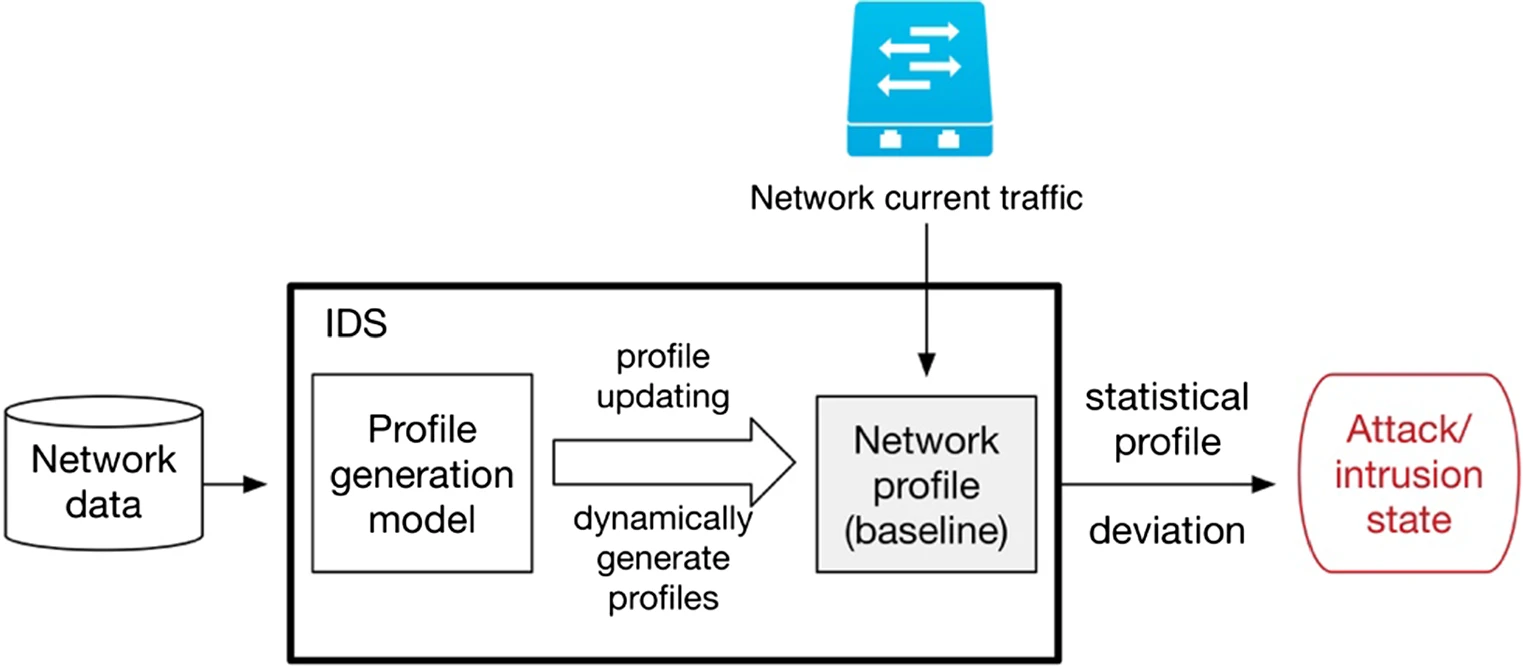
\includegraphics[width=0.6\linewidth]{异常检测技术的通用架构.png}
    \caption{异常检测的通用框架}
    \label{fig:scheme}
  \end{figure}

% 本章还讨论了用于网络入侵检测的数据集的研究挑战。



\section{网络流量异常的定义和分类}
% hawkins(1980)就此我们给出了异常的一个具有本质性的处理定义[3]:异常就是在一个随机数据集中只能表现被认为不具有所属性差异的那些随机数据,使得有人甚至可以由此怀疑这些差异数据实际上本身并非并没有任何随机的处理偏差,而是产生于一种完全不同的处理机制。
Hawkins(1980)\cite{hawkins1980identification}为“异常”下了一个定义:某些数据由于在数据集中表现出差异,因此值得怀疑这些数据不是一般的随机偏差,而是来自完全不同的机制,我们称这些数据为“异常”。例如在道路交通领域,某条道路的车流量突然增多,甚至多至堵塞,又或者突然减少,此时车流量数据就是一个异常。因此网络行为的异常就是指那些与正常的、标准的,我们所预期的行为相异的表现。为了检测网络异常,网络所有者必须有一个预期或正常行为的概念,我们称其为“基线”。要检测网络行为的异常,就需要确保基线持续稳定,如果我们在监测的过程中发现有不寻常的走向,或者有特殊事件出现,就会合理怀疑有外部的蓄意攻击导致网络流量呈现异常,以及监控指标被改变的状况。

% Hawkins(1980)给出了异常的本质性定义\cite{hawkins1980identification}:异常是在数据集中表现出差异的那些数据,使人怀疑这些数据并非随机偏差,而是产生于完全不同的机制。例如在道路交通领域,某条道路的车流量突然增多,甚至多至堵塞,又或者突然减少,此时车流量数据就是一个异常。因此网络行为的异常就是指那些与正常的、标准的,我们所预期的行为相异的表现。为了检测网络异常,网络所有者必须有一个预期或正常行为的概念,我们称其为基线。要检测网络行为的异常,就需要持续监控网络中的意外趋势或事件,那些可能改变网络流量特征或者监控指标的恶意行为。


本文只关注引起网络流量特征变化的恶意行为,而对于系统权限提升,缓冲区溢出等黑客攻击手段暂时不做研究。


网络流量异常具体有哪些类别,学术界没有统一的意见。本文中关注的网络流量异常按照产生意图分为恶意和非恶意两类,其中恶意行为主要有拒绝服务攻击、网络扫描、BGP劫持、网络蠕虫、僵尸网络等;非恶意行为主要有物理故障、突发事件等。接下来我们对这些异常分别进行介绍:

\begin{itemize}
  \item 拒绝服务攻击(Denial of Service,DoS):攻击者往往通过构造大量请求访问目标主机,使其无法处理正常的流量请求,导致正常用户被拒绝服务。
  \item 网络扫描:攻击者在发动网络攻击之前,普遍会先进行网络扫描,否则,黑客可能会向未启动的主机发送恶意报文,从而增加攻击的成本。所以他们总是要先在某个子网范围内扫描出活跃的主机以及可访问的端口。为了以最低代价寻找到可攻击的目标,网络扫描通常是网络攻击的前奏。
  \item BGP劫持:BGP劫持是指通过一个自治系统错误宣称IP为其所有,使得使用边界网关协议维护的互联网路由表的路由器错误地将用户发送的数据传送给非数据传送目的地。
  \item 网络蠕虫:网络蠕虫通过网络和电子邮件进行复制和传播,它们首先搜索并且识别出本身具有缺陷的通信端点,在对这些端点施加攻击后,又经由局部地区的私有网路或者庞大的互联网扩散到其他通信端点。例如“熊猫烧香”及其变种就是蠕虫病毒。
  \item 僵尸网络:僵尸网络指由感染了恶意软件的计算机组成的网络,这些计算机集群由攻击者控制。
  \item 物理故障:物理故障也就是指现实世界中的设备有了损坏,包括但不限于电源与设备未连通、路由器无法传输讯息、链路间无法连接、线缆破损等意外事故。
  \item  突发事件:突发事件是指引起网络瞬时拥塞的事件,有可能是管理员配置错误,也有可能是正常的网络操作,如某网站访问量激增。
\end{itemize}

\section{网络流量异常检测算法}


本节将介绍在异常检测领域主流的一些算法,根据所依赖的技术原理的不同,将这些算法分为了基于分类、基于统计、基于聚类、基于信息论的异常检测算法。

\subsection{基于分类的异常检测算法}

% 基于分类的技术依赖于专家对网络攻击特征的广泛了解。当网络专家向检测系统提供详细的特征时,具有已知模式的攻击一经发起就能被检测出来。这完全依赖于攻击的签名,作为一个系统,只有当网络专家较早地提供了攻击的签名,它才能够检测出攻击。这说明一个只能够检测到它所知道的系统很容易受到新的攻击,而新的攻击会不断出现不同的版本,并且更加隐蔽地发起。即使创建了新的攻击的签名并将其纳入系统中,最初的损失也是不可替代的,而且修复程序非常昂贵。


% 基于分类的方法依赖于建立知识库的正常流量活动特征,并将偏离基线特征的活动视为异常活动。这种方法的优势在于它们能够检测到完全新颖的攻击,
% 假设这些攻击表现出大量的偏离正常基线的情况。需要注意的是,由于知识库中未包含的正常流量被认为是攻击,因此会产生无意中的误报。为了避免这种情况,异常检测技术需要进行训练,以建立正常的活动基线,这个建立基线的过程通常非常耗时,而且还取决于是否有完全正常的流量数据集。在实践中,获得无攻击的流量实例是非常罕见且昂贵的。此外,在如今信息更新变换快速的动态网络环境中,保持正常基线的更新是非常困难的。
本文在现有的大量基于分类的网络异常检测技术中,主要讨论以下三种技术,“支持向量机”(Support Vector Machine,SVM),“贝叶斯”(Bayes)以及“神经网络”(Neural Network, NN)。

\subsubsection{SVM}
Eskin等人\cite{2002AEskin} 引入无监督SVM的概念来检测异常事件。常规的SVM的原理是推导出一个超平面,使得正类样本和负类样本之间的分离余量最大化,将特征空间中的两类数据进行分离。标准的SVM算法是一种监督学习方法,需要标记数据来创建分类规则。而该算法经过改进SVM,试图将整个训练数据集从原点分离出来,找到一个以最大余量将数据实例与原点分离的超平面。

Hu等人\cite{Hu2003Robust} 提出了一种忽略噪声数据的异常检测方法,该方法使用Robust SVM(RSVM)来开发。标准的SVM有一个主要假设,即:“所有的训练样本数据都是独立且相同分布的(i.i.d)”。但是在实际场景中,训练数据往往包含噪声,这就会导致标准SVM会学习出一个高度非线性的决策边界,从而导致通用性较差。有鉴于此,RSVM以类中心的形式加入了平均化技术,使得决策面更加平滑。此外,RSVM另一个优点是能大大降低支持向量的数量,从而减少运行时间,提高效率。

% Taeshik Shon等人\cite{shon2005machine} 提出了一种基于增强支持向量机(Enhanced Support Vector Machines)的异常检测算法。增强支持向量机是该文作者提出的一种新型的支持向量机,该向量机同时具备了传统支持向量机的高性能和单类支持向量机检测新异常的能力。在预处理阶段,检测算法使用数据包过滤器滤除畸形数据包。随后,检测算法使用遗传算法对数据包头的信息进行特征选择。接下来,检测算法利用SOM网络对正常流量进行聚类,并用这些聚类来训练增强支持向量机,从而得到最终的异常检测器。

% Taeshik Shon 等人\cite{shon2005machine}设计了一种此前未有的增强支持向量机(Enhanced Support Vector Machines),这种支持向量机的工作能力结合了以往传统支持向量机与单类支持向量机二者已有的优点,不仅性能优良而且也能较好的识别出新出现的异常。增强支持向量机的训练过程也需要经过预处理的几个步骤,首先是用数据包过滤器排查且删除异常数据包。接着是对数据包头进行处理,这个阶段利用到的是“遗传算法”,会从原始存在的所有特征进行属性选择。在剔除多余无用的特征,且使用自组织映射网络针对正常流量实行聚类之后,会生成样本集合。用这些样本集合训练最新的支持向量机,我们所需的异常检测器就产生出来了。


\subsubsection{贝叶斯}

朴素贝叶斯是一个简单的概率分类器,通常用于网络入侵检测问题。 它将先验信息与样本信息结合起来,并以统计推论的方式进行实施,从而利用概率显示出各种形式的不确定性。 朴素贝叶斯假设了所有输入属性在条件上都是彼此独立的。

Kruegel等人\cite{kruegel2003bayesian} 假设异常检测系统包含许多模型,用于分析一个事件的不同特征。他们指出了在这种系统下异常检测技术造成高误报率的两个主要原因:一是异常检测系统通过将多个概率模型的输出进行汇总,而每个模型往往只给出一个事件的常态/异常的得分或概率,从而导致高误报率;二是异常检测系统无法处理那些不正常但合法的行为,如CPU利用率、内存使用率突然增高等。基于贝叶斯网络的概念,Kruegel\citep{kruegel2003bayesian}指出可以使用一种方法降低误报率,该方法能够正确处理那些在合法范围内稍显不正常的行为。对于一个输入事件的有序流($\symbf{S}=e_1,e_2,e_3...$),异常检测系统决策每个事件是正常还是异常。该决策基于k个模型($\symbf{M}=m_1,m_2,...,m_k$)的输出($o_i|i=1,2,...,k$)和可能的附加信息($\symbf{I}$)。应用贝叶斯网络来识别异常事件,引入根节点,根节点代表一个具有两种状态的变量。一个子节点用于捕捉模型的输出,子节点与根节点相连,预计当输入异常或正常时,输出事件会有所不同。

\subsubsection{神经网络}

神经网络是深度学习的热门技术,早已在多个方面实践成功,但其对计算量的要求很高。神经网络对数据进行分类的优势也可被用于网络异常检测。在网络异常检测领域,神经网络通常会和其他技术进行结合,如统计方法。


Hawkins等人\cite{hawk2002Outlier}提出了一个多层的前馈神经网络,该神经网络可以用来进行异常值的检测。这个多层前馈的神经网络(multi-layer feed-forward neural networks)也就是Replicator Neural Networks。具体而言,它的运行方式是设置了三个隐藏层,夹在输入层和输出层的中间,目标是通过训练,使输出层能以最小的误差重现出输入的数据模式。其原理在于输入层与输出层节点的数量比隐藏层节点的数量要多,因此隐藏层能够具有压缩数据和恢复数据的作用。Replicator Neural Networks的示意图如图~\ref{fig:rnn}所示。

% Hawkins等人\cite{hawk2002Outlier} 提出了一个多层的前馈神经网络,该神经网络可以用来进行异常值的检测。具体来说,Replicator Neural Networks是一个多层前馈的神经网络 (multi-layer feed-forward neural networks),在输入层和输出层之间放置了三个隐藏层,它的目标是通过训练在输出层以最小的误差重现出输入的数据模式。由于该模型中间隐藏层节点的个数少于输入输出层节点的个数,这样就起到了压缩数据和恢复数据的作用。
% Replicator Neural Networks的示意图如图~\ref{fig:rnn}所示。

\begin{figure}
    \centering
    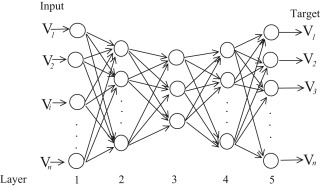
\includegraphics[width=0.6\linewidth]{RNN.jpg}
    \caption{Replicator Neural Networks示意图}
    \label{fig:rnn}
  \end{figure}

  \citet{2001HIDE} 提出了一种分层入侵检测模式,这是他在神经网络的技术基础上搭配了统计方法建立的模型,此系统用一个连续变量($t$)表示神经网络分类器的输出,若变量为1那么当前没有攻击,而-1出现时则是确切的入侵。
  
  除了统计模型,自组织映射(Self-Organizing Map,SOM)亦被用于网络异常检测。Ramadas等人\cite{2003Detecting}提出,由于SOM基于一个假设:即网络攻击可以由不同的神经元组来描述,这些神经元组与其他神经元组相比,在输出神经元图上覆盖更大的区域。因此利用SOM,可以对网络流量进行实时分类。
  
  Poojitha等人\cite{Poojitha2010} 设计出了一种前馈神经网络,使用的训练算法是“反向传播算法”,该模型的要点在于学习出系统无异常期间所表现出的活动模式,并且将违反此期间的行为归类于异常。

\subsection{基于统计的异常检测算法}
从前检测异常是使用假设-检验的方法,也就是要利用统计与概率模型。第一步是预测数据的分布,并从中找到预先认定的“异常”,在此操作下总是使用极值分析或假设检验。也就是说,当前存在基础的一维数据时,首先拟定数据是遵守正态分布的,若有超出均值达到某个范围外的点,就认定是异常点。此操作推广到高维后,假设各个维度相互独立。这类方法的好处是速度比较快,但是因为总要进行“假设”,所以效果不一定很好。因此统计技术的主要挑战是减少固定阈值引起的误报\cite{cormode2010algorithms}。例如,可以使用统计信号处理程序来提高检测率,同时减少误报,如Lakhina等人在主成分分析工作中所做的工作\cite{lakhina2004diagnosing,lakhina2004structural,lakhina2005mining}。

% 早期的异常检测方法往往基于统计与概率模型,也就是假设-检验的方法。首先对数据的分布做出假设,然后找出假设下所定义的“异常”,因此往往使用极值分析或假设检验。比如对最简单的一维数据假设服从正态分布,然后将距离均值某个范围以外的点当做异常点。推广到高维后,假设各个维度相互独立。这类方法的好处速度一般比较快,但是因为存在很强的“假设”,效果不一定很好。因此统计技术的主要挑战是找到减少硬阈值引起的误报产生的方法\cite{cormode2010algorithms}。例如,可以使用统计信号处理程序来提高检测率,同时减少误报,如Lakhina等人在主成分分析工作中所做的工作\cite{lakhina2004diagnosing,lakhina2004structural,lakhina2005mining}。

Nong等人\cite{Nong2010An}基于卡方检验的距离测量方法,将卡方检验的理论应用于异常检测。根据此技术,首先需要建立一个正常事件的基线,然后将偏离统计值的点视为异常。基于chi-square检验统计量的距离测量方法为:
\begin{equation}
    \chi^2 = \sum_{i=1}^n \frac{(X_i - E_i)^2}{E_i}
\end{equation}
其中$X_i$表示的是第$i$个变量的观测值,$E_i$表示的是第$i$个变量的期望值,变量的数量以$n$表示。当一个变量的观测值接近预期时,$\chi^2$的值就会很低。根据$3\sigma$定律,当观测值的$\chi^2$大于$\bar{X^2}+3S_X^2$时,该值被视为异常。

\subsubsection{小波分析} 
小波变换的基本原理涵盖在傅里叶变换的过程当中,起初三角函数基是无限长的,通过小波变换将其变成长度有限且会衰减的小波基。强大的基函数小波,在时间和频率上是局部的,允许被表示的序列和它们的系数之间有密切的联系。如此一来频率得以获取,同时还可以定位到时间。
% 小波分析的重点是对非稳定数据序列进行建模,这种数据序列可能包含在长时间内振幅和频率都会变化的信号。小波变换的基本原理是在傅里叶变换的过程中,将基由无限长的三角函数基换成有限长的会衰减的小波基。小波是强大的基函数,在时间和频率上是局部的,允许被表示的序列和它们的系数之间有密切的联系。这样不仅能够获取频率,还可以定位到时间。


Callegari等人\cite{callegari2011combining}提出了一种利用小波与基线相结合的实时异常检测方法。它是通过提取NetFlow轨迹,并将其转化为ASCII数据文件,进行路由器级别的分析。经过格式化后,通过哈希函数将不同的流量汇总到基线中。然后,将时间序列数据进行小波变换,若发现不连续点则视为异常点。

另一项使用小波的研究是由Hamdi等人\cite{hamdi2007detecting}产生的。它依赖于通过区分危险和非威胁性的异常来识别与攻击相关的异常。这项任务是在周期观测概念的基础上完成的,小波理论被用来分解一维信号,以分析其特殊频率和时间定位。

\subsubsection{主成分分析}
通常情况下,“主成分分析”(Principal component analysis,PCA)方法的用法是将原本在高维空间里面的数据点,以投影法降至低维空间内。但是我们也可以将之用于检测网络流量异常这个领域。该方法的主要原理是将特征空间为$n$的原数据集映射到新的更小的特征空间$k$中,新特征即为主成分(PC),其中$k<<n$,这些 PC是一组正交向量,它们构成了一个$k$维子空间。同理,异常点的判别方法,是将存在于初始空间内的那些数据, 映射到主成分空间,接着再把投影拉回到原始的空间。假如进行投影和重构的数据只包含第一主成分,那么大多数的数据在重构前后误差值不大;但是对于异常点而言,重构之后的误差,相较此前的误差值依然很大。

% 主成分分析(Principal component analysis, PCA)是一种常见的降维方法,也可以用于网络流量异常检测领域。该方法的主要原理是将特征空间为$n$的原数据集映射到新的更小的特征空间$k$中,新特征即为主成分(PC),其中$k<<n$,这些PC是一组正交向量,它们构成了一个$k$维子空间。为了发现异常点,基于主成分分析(PCA)的算法会把原始数据从原始的空间投影到主成分空间,然后再把投影拉回到原始的空间。如果只使用第一主成分来进行投影和重构,对于大多数的数据而言,重构之后的误差是小的;但是对于异常点而言,重构之后的误差依然相对大。

Lakhina等人\cite{lakhina2004diagnosing} 利用主成分分析法对流量测量结果进行二分,分为正常和异常两类。主成分分析是基于将一组网络流量测量所占的高维空间分离成不相干的子空间,分别对应正常和异常的网络条件。PCA 的结果是$k$个子空间,对应正常的网络流量行为,至于剩下的$m$个子空间($m=n-k$) 的组成成分则是异常或噪声。接下来需要通过制定有差异的阈值,使这些结果中的异常流量被检测出来。这时的做法是将每一个新的流量测量值一一投射到$k$和$m$这两个子空间上。

% 利用主成分分析法将测量结果区分为正常和异常两个子空间,能有效地处理流量异常的判定困难。这个方法是基于将一组网络流量测量所占的高维空间分离成不相干的子空间,两个子空间分别对应正常和异常的网络条件。使用主成分分析法得到的是$k$个子空间,这是与符合一般规律的网络流量行为相应的;至于剩余的$m$ 个子空间($m=n-k$),则是与异常和噪声对应。接着再把每一个新的流量测量值投射到这$k$和$m$两种子空间上。这样就可以通过区别开相异的阈值,使得测量出的异常值被从正常测量值中划分开来。

% 利用PCA将流量测量结果有效地分离为正常和异常子空间,解决了网络流量的异常诊断问题。该方法是基于将一组网络流量测量所占的高维空间分离成不相干的子空间,分别对应正常和异常的网络条件。PCA的结果是$k$个子空间,对应正常的网络流量行为,而剩余的$m$个子空间($m=n-k$)则由异常和噪声组成。然后,将每一个新的流量测量值映射到这两个子空间上,这样就可以通过设置不同的阈值将这些测量值划分为正常或异常。

Pascoal等人\cite{pascoal2012robust}提出的异常检测方法采用了鲁棒PCA检测器与鲁棒特征选择算法合并,以获得对不同网络背景和环境的适应性。该鲁棒PCA与经典的PCA方法相反,它对异常值不敏感,并且无需使用可靠标记的数据集进行训练。

Fernandes等人\cite{fernandes2016network}发表了根据统计程序主成分分析生成出的一种异常检测算法。这种算法首先生成一个“使用流量分析的网络段数字签名(DSNSF)”的网络基线,然后将该基线与真实网络流量进行比较以识别异常事件。该系统分析了几天内的历史网络流量数据,从中找出最重要的流量时间间隔,同时对数据集进行了缩减,使新的缩减集能够有效地描述正常的网络行为。然后,以DSNSF作为阈值,通过得到的PCA参数,限制一个区间,偏离阈值的被认为是异常的。该系统共使用七个流量特征,三个IP流量特征(bits/s, packets/s, flows/s)被用来生成DSNSF,四个流量属性(源IP地址、目的IP地址、源TCP/UDP端口和目的TCP/UDP端口)被用来生成一个包含有关异常流量间隔的信息报告。这种方法的缺点是只针对流量属性进行判定异常,只考虑检测基于流量的攻击。


\subsubsection{协方差矩阵}

协方差矩阵是二阶统计,已经被证明是一种强大的异常检测方法。该领域的一个有趣的方向是寻找哪些变量最能标记网络异常,用以提高检测性能。

Yeung等人\cite{yeung2007covariance}采用协方差矩阵分析来检测洪泛攻击。该方法将网络流量建模为协方差矩阵样本,以利用时序样本中包含的统计量达到检测泛洪攻击的目的,直接利用协方差矩阵的变化和相关特征的差异来揭示正常流量与各种类型的洪泛攻击之间的变化。


 Miao Xie等人\cite{xie2014segment}研究了一种基于段的方式处理数据的技术。因为在无线传感器网络(WSNs)中,人们观察到大多数异常事件都会持续相当长的时间。由于现有的异常检测技术通常是以基于点的方式单独处理每个观测值,它们无法可靠和有效地报告在单个传感器节点中出现的这种长期异常。因此该方法采用斯皮尔曼等级相关系数(Spearman's rank correlation coefficient 或 Spearman's $\rho$)和差分压缩概念近似的样本协方差矩阵,以大幅降低计算和通信成本。







% \citet{Christopher2002Service} 提出了一种用于检测异常网络流量的统计处理单元,更具体地说,是为了检测R2L和U2R等罕见的攻击。开发了一种度量方法,使系统能够自动搜索不同服务请求的相同特征。根据以下三个主要特征计算出请求的异常得分。
% 请求的类型;
% 请求的长度;以及
% 有效载荷分布。
% 网络管理员定义了一个阈值,以便对异常请求发出警报。异常得分的计算方法如式(5),其中有效负载分布的权重大于其他属性。(5)
% 基于统计学理论的原理,我们开发了不同类型的技术来检测异常,接下来将讨论。

% 在时间序列异常检测领域,最常见的基于统计的算法为ARIMA,即差分自回归移动平均模型[8]。我们将流量信号分解为两部分,一是遵循一定规律、可预测的正常变化,二是由突发性变化组成、不可预测的异常情况。ARIMA分析和建模用于网络流量预测,能够检测和识别流量异常或异常值。


\subsection{基于信息论的异常检测算法}

信息论是一门以信息量化和冗余分析为核心的数学学科,其前身是1948年Claude E. Shannon在寻求信号处理和通信操作的数据压缩、传输和存储时提出的设想\cite{shannon1948mathematical}。然而,它的应用扩展到许多其他领域,如电子通信、决策支持系统、模式识别等。常用的信息理论测量方法有香农熵、广义熵、条件熵、相对熵、信息增益和信息成本等。信息论应用于异常检测的途径主要是依靠计算流量特征的相互信息或熵值来识别异常分布。

\subsubsection{熵}
% 熵(entropy)是接收的每条消息中包含的信息的平均量,可以理解为不确定性的度量,因为越随机的信源的熵越大。
熵(entropy)在实验中可以当作是不确定性的度量, 因为它是根据收到的每条消息中所包含的信息,平均后得出的量值,所以信息来源越随机,熵的值就越大。
异常检测领域中,熵可以有效地将流量特征描述为分布,例如源/目的端口或IP地址,因为有某些类型的异常会对严重影响这些分布。通过这种方式,可以检测到例如由目的端口熵的变化表示的端口扫描攻击。

Behal等人\cite{behal2017detection}指出,由于DDoS攻击和突发事件会引起网络流量模式的大幅改变,而基于信息理论的熵或散度可以快速捕捉网络流量行为中的这种差异。因此,他们提出了一种利用流量之间的熵差进行异常检测的算法。通过采用了一组泛化的$\phi$-熵和$\phi$-散度,检测合法流量和攻击流量之间的信息距离。经过实验,该算法对于突发事件和DDoS的检测精度较高,而在其他数据集上表现一般。

David等人\cite{david2015ddos} 提出了一种通过快速熵和基于流量的分析来增强对DDoS攻击的检测的方法。作者将观察到的流量汇总成一个单一的流量,并考虑到每个连接在一定时间间隔内的流量数,而不是取每个连接的数据包数。第二步基本上是计算每个连接的流量计数的快速熵。最后,根据快速熵和流量计数的均值和标准差生成一个自适应阈值。阈值随流量模式状况不断更新,提高了检测精度,同时快速熵的使用减少了计算处理时间。

% Amaral等人[129] 提出了一种基于流量特征的异常检测系统,该系统同时使用IP Flow属性和图表示。该算法基于香农熵的一种泛化类型,Tasallis熵。和香农熵的主要区别在于它有一个参数可以定义 对熵的结果有贡献。通过调整异常检测器的敏感性,使其能够适应不同类型的网络,并检测出更多类型的攻击。

% Bhuyan等人[130]提出的工作带来了一种基于离群值的异常检测方法,使用广义熵和互信息来创建一种能够选择相关的、非冗余的特征子集的特征选择技术。作者认为,由于相互信息降低了一个随机变量的不确定性,而广义熵衡量了数据中的不确定性量,因此他们使检测速度更快,更准确。

% 此外,Berezinski等人[131]为了检测现代僵尸网络恶意软件,引入了一种基于香农熵的网络异常检测器。他们的方法创建了一个网络配置文件,它存储了5分钟滑动时间窗口中的最小和最大熵值。这些值被用于与观察到的熵进行比较。这定义了一个阈值,因此,可以识别不同特征分布的异常分散或集中。最后,作者使用流行的分类器,如决策树和贝叶斯网络,以便对异常进行分类。



\subsubsection{KL散度}
KL散度,又称相对熵,通常用于测量一个随机变量$X$的真实概率分布$P$与任意概率分布$Q$($P$的近似)之间的差异。设 $p(x)$、$q(x)$是离散随机变量 $X$ 中取值的两个概率分布,则 $p$ 对 $q$ 的相对熵是:
\begin{equation}
    D_{KL}(p||q) = \sum_x p(x) \log \frac{p(x)}{q(x)} = E_{p(x)} \log \frac{p(x)}{q(x)}
\end{equation}
在机器学习中,$P$往往用来表示样本的真实分布,$Q$用来表示模型所预测的分布。


Xie等人\cite{xie2016distributed} 利用KL散度着重检测了无线传感器网络(WSN)中的一种特殊类型的异常,这种异常会同时出现在邻近节点的集合中,并持续相当长的时间。基于节点的技术在此场景下效果和效率都不尽如人意。作者提出了基于分布式段的递归核密度估计,通过计算两个时间段的概率密度函数的差异,来判断是否发生了异常。同时也为了以较低的通信成本实现分布式估计,作者采用KL散度作为度量方法。利用真实世界的数据集对算法进行评估,结果表明,该算法可以以更低的通信成本实现很好的性能。

Li等人\cite{li2012differential} 以检测无线传感器网络中的异常数据值为目标,提出了一种基于差分KL散度的异常检测方案。该方案首先将整个传感器网络划分为若干个簇,每个簇中的传感器在物理上相互接近,并且具有相似的感知值。然后,在每个簇内使用KL散度,以通过统计测量两个数据集之间的差异来检测异常值。他们的工作取得了良好的检测率和较低的误报率,同时比其他文献中的类似研究消耗更少的CPU、内存等资源。



% Ambusaidi等人(2014)中提出了一种基于非线性相关系数(NCC)的相似性测量方法,以提取网络流量之间的线性和非线性相关性。提取的相关信息用于检测恶意网络行为。Pearson׳s相关系数是一种基本的线性相关方法,用于找出两个变量之间的依赖关系(Ahmed等,2015c),然而,在一些数据集中,不同变量之间存在非线性相关,如网络流量中。NCC由Wang等(2005)定义,如式(18),其中和为变量X和Y的修正熵。

% 给定一组m个正常训练数据实例,首先计算NCC。对于任何传入实例,传入实例与正常实例之间的NCC记录为 。对于用户定义的阈值σ,其范围在0和1之间,如果NCC的差异大于σ,则认为一个传入流量实例是异常的(19)。


% 在Tan等(2014a)中,针对DoS攻击检测,提出了一个利用多元相关分析(MCA)的系统,通过提取网络流量特征之间的几何相关性,来实现网络流量的精确特征分析。检测过程主要包含三个步骤,如图6所示。在步骤1中,在一个明确的时间区间内生成基本特征。第2步包含多元相关分析,应用 "三角区域图生成 "模块,提取第一步得出的每个流量实例中两个不同特征之间的相关性。第三步是基于训练和测试阶段的决策。


% 基于这些知识,可以建立适当的异常检测模型。有监督的异常检测技术需要先有一个训练数据集,再有一个测试数据来评估模型的性能。在这种情况下,首先,使用信息理论措施来确定模型是否适合测试新数据集。Noble和Cook(2003)在基准DARPA和UNM审计数据集上进行了实验,以证明信息理论措施的效用,并得出结论,它们可以用来创建高效的异常检测模型,也可以用来解释它们的性能

% Tan等人(2014a)中的多变量相关分析方法的概念被纳入到网络流量实例的表征中,并将其转换为相应的图像。这些图像被用于DoS攻击检测,基于一个广泛使用的异构度量,即地球移动者距离(Earth Mover׳s Distance,EMD)(Rubner等,1998)。EMD考虑了跨区域匹配,比其他一些著名的异同度测量方法更准确地评估了分布之间的异同度。

\subsection{基于聚类的异常检测算法}

% 聚类分析是把彼此相似的对象分成不同的组别,组内的对象是相似的(相关的),而不同组之间是不同的(不相关的)。如果组内的相似性越大,组间的差别越大,说明聚类的效果越好。因此,聚类技术可以用于离群值检测(Outlier Detection),识别出与正常组别相距较“远”的值,判定为异常值/离群值\cite{2012Cluster}。聚类算法通常是基于距离/密度发现异常点。其关键步骤在于给每个数据点都分配一个离散度,针对给定的数据集,对其中的任意一个数据点,如果在其局部邻域内的点都很密集,那么认为此数据点为正常数据点,而异常点则是距离正常数据点最近邻的点都比较远的数据点。通常由阈值进行距离远近的界定。


Rajasegar等人\cite{2014Hyperspherical}发明了一种聚类算法,是根据分布式超球面集群得出的,主要作用在于检查测试无线传感器网络中有无异常。
检测过程是以聚类法进行建模,对象是每个端点的流量数据。建模后还要使用k 个最近邻(KNN)集群的平均集群之间的距离去辨认出异常集群,辨认后就可以将数据向量分类为正常或异常。该算法的特点是操作过程在分布式系统中,通过传感器端点指出集群聚类的信息。在与其他端点传递信息之前,先凭借中间节点的先行合并,能使得通信开销降至最低。
% 提出了一种基于分布式超球面集群的聚类算法,用于检测无线传感器网络中的异常。
% 该算法利用聚类对每个节点的流量数据进行建模,通过使用k个最近邻(KNN)集群的平均集群间距来识别异常集群,就可以将数据向量分类为正常或异常。该算法的特点是在分布式系统下进行,传感器节点上报集群聚类的信息,在与其他节点通信之前,由中间节点先行合并,从而使得通信开销最小化。


K-means 虽然有局部收敛性和在簇中心节点选择上具有敏感性这些缺点。但是它仍然是一种经典的聚类技术,能够将数据划分为不同的类别。由于这种技术十分热门,有相当多的技术人员尝试着想借助其他技术来优化k-means,去改善k-means的不足之处。Karami等人\cite{2015Karami} 就设计了一种基于“粒子群优化”(particle swarm optimization,PSO) 和k-means 与局部优化混合的模糊异常检测系统,以确定最优的簇数。



Carvalho等人\cite{carvalho2016unsupervised} 开发了一种主动式网络监控系统,可以检测异常事件,减少决策中的人工干预和错误概率。他们提出一种创建网络基线轮廓DSNSF(使用流量分析的网段数字签名)的方法。该方法通过修改蚁群优化算法,使用聚类方法描述正常的网络使用情况,该方法称为ACODS。ACODS在大量高维输入数据中,通过无监督学习机制优化提取行为模式,对网络流量发现进行表征。然后为了检测异常行为,他们首先计算每个时间区间内真实流量与正常曲线的相似度;然后计算序列之间的距离,并提供基于距离的测量方法。
作者所提出的告警系统采用七种流量属性(Bits, Bytes, Flows, Origin IP, Destination IP, Origin Port, Destination Port)工作,利用熵来计算IP地址和端口特征的相关信息。当检测到异常时,ACODS会提供一份包含IP流量信息的完整报告,说明每个属性对检测到的异常时间间隔的影响。ACODS具有平方复杂度,导致解的收敛要经过多次迭代,作者试图通过使用局部搜索和信息素更新来缓解。

Dromard等人\cite{dromard2016online} 所设计的无监督异常检测器,是建立在网格增量聚类算法和离散时间滑动窗口之上的。网格增量聚类在众多聚类算法当中效率拔群,因为后者只更新之前的特征空间分区,而不是每当增加或删除很少的点时,就对整个空间进行重新分区。也因此,网格增量聚类的使用是在帮系统减少繁复性,并且使其在实时检测方面效能更强。最后系统合并这些更新的分区,用以识别最不相似的异常值。

% 提出了一种基于网格增量聚类算法和离散时间滑动窗口的无监督异常检测器。网格增量聚类比常规的聚类算法更有效率,因为后者只更新之前的特征空间分区,而此前的做法是每当对点的数目进行增删时,哪怕更改的点不多,也会对整个空间做重新分区的处理。增量网格聚类的使用有助于降低系统复杂度,从而使其在实时检测方面更加可行。最后系统合并这些更新的分区,用以识别最不相似的异常值。


Syarif等人\cite{2012syarif} 在NSL-KDD数据集上系统对比了各种聚类算法的性能,他们选出了5种应用最广泛的聚类算法:k-means、改进的k-means、k-medoids、EM算法和基于距离的异常检测算法。实验表明,在同等水平的误报率情况(约21\%)下,基于距离的异常检测算法效果最好,准确率为80.15\%,k-means算法效果最差,准确率为57.81\%。
% 表\ref{聚类算法}展示了这些算法在NSL-KDD数据集下的性能表现。

% \begin{table}[]
%   \caption{聚类算法在NSL-KDD数据集的性能对比}
%   \label{聚类算法}
%     \centering
%     \begin{tabular}{@{}clllclcl@{}}
%     \toprule
%     \multicolumn{4}{c}{Algorithm}                          & \multicolumn{2}{c}{Accuracy(\%)} & \multicolumn{2}{c}{False positive(\%)} \\ \midrule
%     \multicolumn{4}{c}{k-means}                            & \multicolumn{2}{c}{57.81}        & \multicolumn{2}{c}{22.95}              \\
%     \multicolumn{4}{c}{Improved k-means}                   & \multicolumn{2}{c}{65.4}         & \multicolumn{2}{c}{21.52}              \\
%     \multicolumn{4}{c}{k-medoids}                          & \multicolumn{2}{c}{76.71}        & \multicolumn{2}{c}{21.83}              \\
%     \multicolumn{4}{c}{EM clustering}                      & \multicolumn{2}{c}{78.06}        & \multicolumn{2}{c}{20.74}              \\
%     \multicolumn{4}{c}{Distance-based   anomaly detection} & \multicolumn{2}{c}{80.15}        & \multicolumn{2}{c}{21.14}              \\ \bottomrule
%     \end{tabular}
%     \end{table}
% 异常检测方法的一些主要局限性基本上是:没有标签数据;发现新的未知异常模式;噪声数据;高误报率。为了克服这些问题,Bigdeli等人[103]提出了一种基于增量两层集群的异常检测结构。其核心思想是对网络数据进行聚类,并将这些聚类表示为高斯混合物模型,因此该模型可以对新的实例进行分类,也可以检测并忽略冗余的实例。此外,针对误报率较高的问题,采用集体标记的方法,对新入库实例进行集体标记和增量标记。


% 聚类指的是无监督学习算法,它不需要预先标记数据来提取相似数据实例的分组规则(Jain等,1999)。虽然有不同类型的聚类技术,但我们讨论常规聚类和共聚类对网络异常检测的有用性。常规聚类和共聚类的区别在于行和列的处理。常规聚类技术如k-means(Ahmed和Naser,2013)考虑数据集的行进行聚类,而共聚类则同时考虑数据集的行和列来产生聚类(Ahmed等人,2015d)。

% 下面简单讨论一下使用聚类检测异常时总是要做的三个关键假设。
% 假设1:由于我们只能创建正常数据的聚类,因此,后续任何与现有正常数据聚类不相适应的新数据都被认为是异常数据;例如,由于基于密度的聚类算法不包括聚类内的噪声(Ester等人,1996),噪声被认为是异常数据。

% 假设2:当一个簇同时包含正常数据和异常数据时,已经发现正常数据靠近最近的簇中心点,但异常数据远离中心点(Ahmed和Naser,2013)。在这种假设下,异常事件使用距离得分来检测。

% 假设3:在一个具有不同大小的聚类中,较小和较稀疏的聚类可以被认为是异常的,较厚的聚类是正常的。属于大小和/或密度低于阈值的聚类的实例被认为是异常的。


% Münz等人(2007)对异常数据采用的方法非常直接。他们使用k-means聚类来生成正常和异常聚类。一旦实现聚类,就使用以下假设进行分析。

% 如果一个实例比异常簇中心点更接近正常,则该实例被列为正常,反之亦然。


% 如果实例与中心点之间的距离大于预定义的阈值(dmax),则该实例被视为异常;以及


% 如果一个实例比正常聚类中心点更接近异常聚类中心点,或者它与正常聚类中心点的距离大于预定义的阈值,则被视为异常。


% Petrovic等(2006)提出了一种基于聚类评价技术组合的聚类标签策略。将Davies-Bouldin聚类评价指数和聚类中心直径的比较结合起来,以充分应对攻击向量的特性。他们考虑了相应聚类的紧凑性和它们之间的分离度,以及区分分析网络中 "正常 "和 "异常 "行为的主要参数。然而,他们并没有解释他们的k-means聚类使用k=2的原因。根据他们的方法,攻击向量通常非常相似,如果不是完全相同的话;例如,在大规模攻击的情况下,相应的聚类是非常紧凑的,这种聚类的Davies-Bouldin指数要么是0(当非攻击聚类是空的时候),要么是非常接近0。考虑到攻击向量之间的预期相似性,因为攻击聚类的中心点的直径预期比非攻击聚类的直径小,他们可以区分正常和异常的聚类。

% Portnoy等(2001)提出了基于宽度的聚类来对数据实例进行分类。宽度是恒定的,对所有聚类都保持不变。一旦进行聚类,基于正常实例在整个数据集中占压倒性比例的假设,N\%的聚类是正常的,其余是异常的。利用这一假设,Leung和Leckie(2005)提出了一种基于密度和网格的聚类算法,该算法适用于无监督的异常检测。



% \subsection{基于深度学习的异常检测算法}
% 随着深度学习的兴起,越来越多的学者尝试用深度学习算法来进行异常检测,尤其是针对时间序列数据,深度学习模型往往表现出惊人的效果。
% 常用的深度学习算法为变分编码器、神经网络[6][14]、生成对抗网络、LSTM[17]、RNN[3][4][10][12][13][15]等。以变分自动编码器(Variational Auto-Encoder)[5]为例,其利用自编码器的重构误差和局部误差,针对时间序列的异常检测的场景,达到了很好的效果。

% \section{异常检测领域开源数据集介绍}
% 数据集主要由KDDCUP99, CICIDS等。网络流量异常检测领域最为经典的数据集当属KDD99,但是这个数据集年代过于久远,对于现在的网络环境早已不适用。 NSL-KDD是为了解决KDD'99数据集的一些固有问题而提出的数据集。虽然,这个新版本的KDD数据集仍然存在McHugh所讨论的一些问题,并且可能不能完美地代表现有的真实网络,但由于缺乏基于网络的IDS的公共数据集,我们相信它仍然可以作为一个有效的基准数据集来帮助研究人员比较不同的入侵检测方法。

% 此外,NSL-KDD训练集和测试集的记录数量是合理的。这一优势使得在完整的集合上运行实验是经济实惠的,而不需要随机选择一小部分。因此,不同研究工作的评价结果将具有一致性和可比性。

% % CICIDS2017数据集包含了良性的和最新的常见攻击,与真实的现实世界数据(PCAPs)相似。它还包括使用CICFlowMeter进行网络流量分析的结果,并根据时间戳、源和目的IP、源和目的端口、协议和攻击(CSV文件)对流量进行了标注。同时还提供了提取的特征定义。

% 生成真实的背景流量是我们构建这个数据集的首要任务。我们使用了我们提出的B-Profile系统(Sharafaldin,等人,2016)来对人类交互的抽象行为进行剖析,并生成自然的良性背景流量。对于这个数据集,我们基于HTTP、HTTPS、FTP、SSH和电子邮件协议建立了25个用户的抽象行为。

% 数据采集期从2017年7月3日(周一)上午9点开始,到2017年7月7日(周五)下午5点结束,共5天。其中周一为正常日,只包括良性流量。实施的攻击包括蛮力FTP、蛮力SSH、DoS、Heartbleed、Web攻击、渗透、僵尸网络和DDoS。它们在周二、周三、周四和周五的上午和下午都被执行过。

% % 在我们最近的数据集评估框架中(Gharib等人,2016),我们确定了建立一个可靠的基准数据集所必需的11个标准。之前的IDS数据集都无法覆盖这11项标准的全部内容。在下文中,我们简要地概述了这些标准。

% THU-IDS 清华校园网数据集,该数据集为真实流量,将于第三章进行介绍。

% https://www.unb.ca/cic/datasets/nsl.html
% \section{异常检测算法对比}
% 对比
% 不同机器学习方法在NSL-KDD数据集上的效果,
\section{现有异常检测算法存在的问题}
截至目前, 异常检测算法的种类已经不可胜数,其中所使用的原理都有差别,针对的领域也各异,流量特征自然也不一样。但通过本文的实验对比我们可以看出,在应对大规模、应用类型多、异常流量是常态且多种异常相互叠加的场景下,现有异常检测算法大多仍存在以下缺陷:

\begin{enumerate}
  \item 面对海量数据规模时,无法或很难做到实时性;
  \item 应用类型多导致的流量特征复杂,因此很难达到较高的检测率和较低的误报率;
  \item 目前的检测算法大多是对异常检测进行二分类,这就导致尽管我们知道数据中存在异常,但是想知道异常的类别以及异常定位,却无法完成。即异常被检测到后,算法无法给出运维人员指导性意见来具体应对。
\end{enumerate}

根据以上几点缺点,想要利用目前已知的异常检测算法精准地判断出异常种类,还是不太现实。确切地说,目前大多数异常检测算法还只停留在证实可行性的阶段。

\section{本章小结}
本章是相关工作综述,首先介绍了网络流量异常的定义和分类,然后按照不同的类别综述了网络流量异常检测的常用算法。最后总结了现有异常检测算法存在的主要问题。


% !TeX root = ../thuthesis-example.tex

\chapter{数据集分析与对比}
\section{开源数据集}
\subsection{UNSW-NB15}
UNSW-NB15 数据集是 2015 年澳大利亚网络安全中心使用 IXIA Perfect Storm工具模拟网络环境流量而生成的一个数据集。相比于 KDD99 是一个更新的数据集,因此更能代表真实的网络流量。UNSW-NB15 数据集中包括 100GB的.pcap 格式的原始网络流量,同时还有 4 个经过特征提取的 csv 文件,分别是UNSW-NB15\_1.csv  、 UNSW-NB15\_2.csv 、 UNSW-NB15\_3.csv  和   UNSW-NB15\_4.csv,一共是 2540044 条数据,同时该数据集提出了与 KDD99 较为不同的特征,这些特征更为符合当前的网络协议模式。 UNSW-NB15 一共包含有 10 个分类,一个正常类别和 9 个攻击类别,其具体描述和类别数目如下表所示: 
% 表 3.2 攻击类型描述和数目 

\flushleft{

    \begin{table}[H]
        \begin{tabular}{|p{0.1\textwidth}<{\centering} |p{0.7\textwidth}<{\centering} |p{0.1\textwidth}<{\centering}|}
        % \begin{tabular}{lp{3cm}p{9cm}p{3cm}}
        \toprule 
        类别 & 类别描述                                                                       & 样本数量    \\ \midrule 
        Normal  & 正常流量                                                                       & 2218761 \\ \hline
        Fuzzers & 攻击者从命令行或以报文的形式发送大量随机生成的输入序列。攻击者试图发现操作系统、程序或网络中的安全漏洞,并使这些资源挂起一段时间,甚至可以使它们崩溃 & 24246   \\ \hline
        Analysis & 这类攻击是指通过端口扫描、恶意 web 脚本
    (如 HTML 文件渗透)和发送垃圾邮件等各种
    方式渗透到 web 应用程序的各种入侵等。 & 2677 \\ \hline
    Backdoor & 这类攻击中攻击者可以绕过正常的身份验证
    并获得对系统的未授权远程访问。黑客利用
    后门程序安装恶意文件,修改代码或获得对
    系统或数据的访问。 &
    2329 \\ \hline
    DoS & 攻击者使某些计算或内存资源过于繁忙或占
    据全部资源而无法处理合法请求或者拒绝合
    法用户对计算机的访问。 &
    16353 \\ \hline
    Exploit & 利用操作系统或软件中的软件漏洞、漏洞或
    故障进行入侵的行为。攻击者利用软件的知
    识发动攻击,意图对系统造成危害。 &
    44525 \\ \hline
    Generic & 针对密码系统的攻击,试图破坏安全系统的
    密钥。它独立于密码系统的实现细节。不考
    虑块密码的结构。例如,生日攻击是一种将
    哈希函数视为黑盒的通用攻击。 &
    215481 \\ \hline
    Reconnaissance & 为了绕过目标计算机网络的安全控制而收集
    其信息的攻击。它可以被定义为一个探针,
    是发起进一步攻击的初步步骤。攻击者使用
    各种扫描手段来收集系统信息。在收集到足
    够的信息后,可以发起后续的攻击。 &
    13987 \\ \hline
    Shellcode & Shellcode 作为负载在目标机器执行,来挖掘
    该软件的漏洞。之所以称作 Shellcode 是因为
    启动了受到攻击者控制的命令行 shell。 &
    1511 \\ \hline
    Worm & 蠕虫是一种恶意程序或恶意软件,它可以复
    制自己并传播到其他计算机。 &
    174 \\  
        \bottomrule
        \end{tabular}
        \end{table}

}


 
UNSW-NB15 数据集一共包含 47 个特征,其中时间戳,IP 地址,端口号等特
征对训练无用,因此有效的特征一共 41 个。 
下面对这些特征做一个概括的说明。按照数据集作者的思路,可以分为基本
特征,内容特征,时间特征和额外生成的特征这几类。这里从另外一种思路进行
重新归类可以分为以下几类。


\begin{table}[H]
    \caption{与协议相关的特征}
    \centering
    \begin{tabular}{|l|l|}
    \hline
    特征名称                  & 特征描述                      \\ \hline
    proto                 & 传输层协议                     \\ \hline
    service               & 应用层协议                     \\ \hline
    sttl                  & 从源发出的报文的 time to live     \\ \hline
    dttl                  & 从目的发出的报文的 time to live 字段 \\ \hline
    stcpb                 & 源 tcp 报文的初始序列号            \\ \hline
    dtcpb                 & 目的 tcp 报文的初始序列号           \\ \hline
    swin                  & 源 tcp 报文的窗口字段             \\ \hline
    dwin                  & 目的 tcp 报文的窗口字段            \\ \hline
    res\_bdy\_len         & http 响应内容的长度              \\ \hline
    ct\_flw\_http\_method & 会话中 http 方法字段的计数          \\ \hline
    is\_ftp\_login        & 是否有 ftp 的登录               \\ \hline
    ct\_ftp\_cmd          & 会话中 ftp 命令的计数             \\ \hline
    trans\_depth          & http 服务的连接深度              \\ \hline
    \end{tabular}
    \end{table}

\begin{table}[H]
    \caption{与时间相关的特征}
    \centering
    \begin{tabular}{|l|l|}
    \hline
    dur     & 会话的持续时间                        \\ \hline
    tcprtt  & tcp 三次握手的 rtt(round trip time) \\ \hline
    synack  & 第一次发送到确认的时间                    \\ \hline
    ackdat  & 确认之后返回的时间                      \\ \hline
    sintpkt & 源报文的间隔时间的平均值                   \\ \hline
    dintpkt & 目的报文间隔时间的平均值                   \\ \hline
    sjit    & 源报文间隔时间的标准差(jitter)            \\ \hline
    djit    & 目的报文间隔时间的标准差                   \\ \hline
    sload   & 源报文的吞吐量                        \\ \hline
    dload   & 目的报文的吞吐量                       \\ \hline
    \end{tabular}
    \end{table}

    \begin{table}[H]
        \caption{与报文大小相关的特征}
        \centering
        \begin{tabular}{|l|l|}
        \hline
        sbytes  & 会话中从源发出的总字节数  \\ \hline
        dbytes  & 会话中从目的发出的总字节数 \\ \hline
        smeansz & 会话中源报文的平均大小   \\ \hline
        dmeansz & 会话中目的报文的平均大小  \\ \hline
        spkts   & 会话中源的报文总数     \\ \hline
        dpkts   & 会话中目的报文总数     \\ \hline
        \end{tabular}
        \end{table}

\begin{table}[H]
    \caption{与连接状态相关的特征}
    \centering
    \begin{tabular}{|l|l|}
    \hline
    sloss & 源的丢包数和重传数之和  \\ \hline
    dloss & 目的的丢包数和重传数之和 \\ \hline
    state & 会话的状态和相应的协议  \\ \hline
    \end{tabular}
    \end{table}

\begin{table}[H]
    \caption{额外构造的特征}
    \centering
    \begin{tabular}{|l|l|}
    \hline
    ct\_srv\_src                & 根据最后一条报文的时间排序,每 100 条记录中源ip 与服务都相同的会话计数(下面省略每 100 条)  \\ \hline
    ct\_srv\_dst                & 目的 IP 与服务都相同的会话计数         \\ \hline
    ct\_dst\_ltm                & 目的 IP 相同的会话计数             \\ \hline
    ct\_src\_ltm                & 源 IP 相同的会话计数              \\ \hline
    ct\_src\_dport\_ltm         & 源 IP 和目的端口都相同的会话计数        \\ \hline
    ct\_dst\_sport\_ltm         & 目的 IP 和源端口都相同的会话计数        \\ \hline
    ct\_dst\_src\_ltm           & 目的 IP 和源 IP 都相同的会话计数      \\ \hline
    ct\_state\_ttl              & 对于每一个状态,ttl 值的范围          \\ \hline
    is\_sm\_ips\_ports          & 源 ip 与目的 ip,源端口和目的端口是否都相同 \\ \hline
    \end{tabular}
    \end{table}
 
可以看到,UNSW-NB15 数据集大多数特征都有较为清晰的定义,因此可以
用做流量数据特征提取的标准。 

\subsection{CICIDS2017}
CICIDS数据集特征介绍如下:(修改成跨页表格)


List of extracted features and descriptions: \\

% \begin{longtable}{cc}
%     \begin{tabular}
%       abc & dfg
% \end{tabular}
% \end{longtable}
Flow duration  单条流持续时间/微秒 \\
total Fwd Packet		发送方packet数量 \\
total Bwd packets		接收方packet数量 \\
total Length of Fwd Packet	发送方packet总长度 \\
total Length of Bwd Packet	接收方packet总长度 \\
Fwd Packet Length Min 		发送方packet最小长度 \\
Fwd Packet Length Max 		发送方packet最大长度 \\
Fwd Packet Length Mean		发送方packet平均长度 \\
Fwd Packet Length Std		发送方packet长度标准差 \\
Bwd Packet Length Min		接收方packet最小长度 \\
Bwd Packet Length Max		接收方packet最大长度 \\
Bwd Packet Length Mean		接收方packet平均长度 \\
Bwd Packet Length Std		接收方packet长度标准差 \\
Flow Bytes/s			bps \\
Flow Packets/s			pps  \\
Flow IAT Mean			一条流中包平均间隔时间 \\
Flow IAT Std			一条流中包间隔时间的标准差 \\
Flow IAT Max			一条流中两个packet最大间隔时间 \\
Flow IAT Min			一条流中两个packet最小间隔时间 \\
Fwd IAT Min			发送方两个packet最小间隔时间\\
Fwd IAT Max			发送方两个packet最大间隔时间 \\
Fwd IAT Mean			发送方两个packet平均间隔时间 \\
Fwd IAT Std			发送方两个packet间隔时间的标准差 \\
Fwd IAT Total   		发送方两个packet总间隔时间\\
Bwd IAT Min			接收方两个packet最小间隔时间\\
Bwd IAT Max			接收方两个packet最大间隔时间\\
Bwd IAT Mean			接收方两个packet平均间隔时间 \\
Bwd IAT Std			接收方两个packet间隔时间的标准差 \\
Bwd IAT Total			接收方两个packet总间隔时间 \\
Fwd PSH flags			发送方PSH标志位出现次数(0 for UDP) \\
Bwd PSH Flags			接收方PSH标志位出现次数(0 for UDP)\\
Fwd URG Flags			发送方URG标志位出现次数(0 for UDP) \\
Bwd URG Flags			接收方URG标志位出现次数(0 for UDP) \\
Fwd Header Length		发送方header占用的总字节数 \\
Bwd Header Length		接受方header占用的总字节数 \\
FWD Packets/s			发送方pps \\
Bwd Packets/s			接收方pps \\
Packet Length Min 		packet最小长度 \\
Packet Length Max		packet最大长度 \\
Packet Length Mean 		packet平均长度 \\
Packet Length Std		packet长度标准差 \\
Packet Length Variance  	packet长度方差 \\
FIN Flag Count 			FIN标志位出现次数 \\
SYN Flag Count 			SYN标志位出现次数 \\
RST Flag Count 			RST标志位出现次数 \\
PSH Flag Count 			PUSH标志位出现次数 \\
ACK Flag Count 			ACK标志位出现次数 \\
URG Flag Count 			URG标志位出现次数 \\
CWR Flag Count 			CWR标志位出现次数 \\
ECE Flag Count 			ECE标志位出现次数 \\
down/Up Ratio			下载/上传比 \\
Average Packet Size 		packet平均大小 \\
Fwd Segment Size Avg 		Average size observed in the forward direction \\
Bwd Segment Size Avg 		Average number of bytes bulk rate in the backward direction \\
Fwd Bytes/Bulk Avg		Average number of bytes bulk rate in the forward direction \\
Fwd Packet/Bulk Avg		Average number of packets bulk rate in the forward direction \\
Fwd Bulk Rate Avg 		Average number of bulk rate in the forward direction \\
Bwd Bytes/Bulk Avg		Average number of bytes bulk rate in the backward direction \\
Bwd Packet/Bulk Avg 		Average number of packets bulk rate in the backward direction \\
Bwd Bulk Rate Avg		Average number of bulk rate in the backward direction \\
Subflow Fwd Packets		The average number of packets in a sub flow in the forward direction \\
Subflow Fwd Bytes		The average number of bytes in a sub flow in the forward direction \\
Subflow Bwd Packets		The average number of packets in a sub flow in the backward direction \\
Subflow Bwd Bytes		The average number of bytes in a sub flow in the backward direction \\
Fwd Init Win bytes		The total number of bytes sent in initial window in the forward direction \\
Bwd Init Win bytes		The total number of bytes sent in initial window in the backward direction \\
Fwd Act Data Pkts		Count of packets with at least 1 byte of TCP data payload in the forward direction \\
Fwd Seg Size Min		Minimum segment size observed in the forward direction \\
Active Min			Minimum time a flow was active before becoming idle \\
Active Mean			Mean time a flow was active before becoming idle \\
Active Max			Maximum time a flow was active before becoming idle \\
Active Std			Standard deviation time a flow was active before becoming idle \\
Idle Min			Minimum time a flow was idle before becoming active \\
Idle Mean			Mean time a flow was idle before becoming active \\
Idle Max			Maximum time a flow was idle before becoming active \\
Idle Std			Standard deviation time a flow was idle before becoming active \\


Flow duration			Duration of the flow in Microsecond \\
total Fwd Packet		Total packets in the forward direction \\
total Bwd packets		Total packets in the backward direction \\
total Length of Fwd Packet	Total size of packet in forward direction \\
total Length of Bwd Packet	Total size of packet in backward direction \\
Fwd Packet Length Min 		Minimum size of packet in forward direction \\
Fwd Packet Length Max 		Maximum size of packet in forward direction \\
Fwd Packet Length Mean		Mean size of packet in forward direction \\
Fwd Packet Length Std		Standard deviation size of packet in forward direction \\
Bwd Packet Length Min		Minimum size of packet in backward direction \\
Bwd Packet Length Max		Maximum size of packet in backward direction \\
Bwd Packet Length Mean		Mean size of packet in backward direction \\
Bwd Packet Length Std		Standard deviation size of packet in backward direction \\
Flow Bytes/s			Number of flow bytes per second \\
Flow Packets/s			Number of flow packets per second  \\
Flow IAT Mean			Mean time between two packets sent in the flow \\
Flow IAT Std			Standard deviation time between two packets sent in the flow \\
Flow IAT Max			Maximum time between two packets sent in the flow \\
Flow IAT Min			Minimum time between two packets sent in the flow \\
Fwd IAT Min			Minimum time between two packets sent in the forward direction \\
Fwd IAT Max			Maximum time between two packets sent in the forward direction \\
Fwd IAT Mean			Mean time between two packets sent in the forward direction \\
Fwd IAT Std			Standard deviation time between two packets sent in the forward direction \\
Fwd IAT Total   		Total time between two packets sent in the forward direction \\
Bwd IAT Min			Minimum time between two packets sent in the backward direction \\
Bwd IAT Max			Maximum time between two packets sent in the backward direction \\
Bwd IAT Mean			Mean time between two packets sent in the backward direction \\
Bwd IAT Std			Standard deviation time between two packets sent in the backward direction \\
Bwd IAT Total			Total time between two packets sent in the backward direction \\
Fwd PSH flags			Number of times the PSH flag was set in packets travelling in the forward direction (0 for UDP) \\
Bwd PSH Flags			Number of times the PSH flag was set in packets travelling in the backward direction (0 for UDP) \\
Fwd URG Flags			Number of times the URG flag was set in packets travelling in the forward direction (0 for UDP) \\
Bwd URG Flags			Number of times the URG flag was set in packets travelling in the backward direction (0 for UDP) \\
Fwd Header Length		Total bytes used for headers in the forward direction \\
Bwd Header Length		Total bytes used for headers in the backward direction \\
FWD Packets/s			Number of forward packets per second \\
Bwd Packets/s			Number of backward packets per second \\
Packet Length Min 		Minimum length of a packet \\
Packet Length Max		Maximum length of a packet \\
Packet Length Mean 		Mean length of a packet \\
Packet Length Std		Standard deviation length of a packet \\
Packet Length Variance  	Variance length of a packet \\
FIN Flag Count 			Number of packets with FIN \\
SYN Flag Count 			Number of packets with SYN \\
RST Flag Count 			Number of packets with RST \\
PSH Flag Count 			Number of packets with PUSH \\
ACK Flag Count 			Number of packets with ACK \\
URG Flag Count 			Number of packets with URG \\
CWR Flag Count 			Number of packets with CWR \\
ECE Flag Count 			Number of packets with ECE \\
down/Up Ratio			Download and upload ratio \\
Average Packet Size 		Average size of packet \\
Fwd Segment Size Avg 		Average size observed in the forward direction \\
Bwd Segment Size Avg 		Average number of bytes bulk rate in the backward direction \\
Fwd Bytes/Bulk Avg		Average number of bytes bulk rate in the forward direction \\
Fwd Packet/Bulk Avg		Average number of packets bulk rate in the forward direction \\
Fwd Bulk Rate Avg 		Average number of bulk rate in the forward direction \\
Bwd Bytes/Bulk Avg		Average number of bytes bulk rate in the backward direction \\
Bwd Packet/Bulk Avg 		Average number of packets bulk rate in the backward direction \\
Bwd Bulk Rate Avg		Average number of bulk rate in the backward direction \\
Subflow Fwd Packets		The average number of packets in a sub flow in the forward direction \\
Subflow Fwd Bytes		The average number of bytes in a sub flow in the forward direction \\
Subflow Bwd Packets		The average number of packets in a sub flow in the backward direction \\
Subflow Bwd Bytes		The average number of bytes in a sub flow in the backward direction \\
Fwd Init Win bytes		The total number of bytes sent in initial window in the forward direction \\
Bwd Init Win bytes		The total number of bytes sent in initial window in the backward direction \\
Fwd Act Data Pkts		Count of packets with at least 1 byte of TCP data payload in the forward direction \\
Fwd Seg Size Min		Minimum segment size observed in the forward direction \\
Active Min			Minimum time a flow was active before becoming idle \\
Active Mean			Mean time a flow was active before becoming idle \\
Active Max			Maximum time a flow was active before becoming idle \\
Active Std			Standard deviation time a flow was active before becoming idle \\
Idle Min			Minimum time a flow was idle before becoming active \\
Idle Mean			Mean time a flow was idle before becoming active \\
Idle Max			Maximum time a flow was idle before becoming active \\
Idle Std			Standard deviation time a flow was idle before becoming active \\
\section{校园网真实数据集}
校园网规模巨大,每天有海量的数据,这给我们的分析带来了很多困难。
首先输入数据是pcap形式的流量数据,如下图~\ref{fig:wireshark}所示,包含每个数据包的详细信息,如五元组、报文内容

\begin{figure}
    \centering
    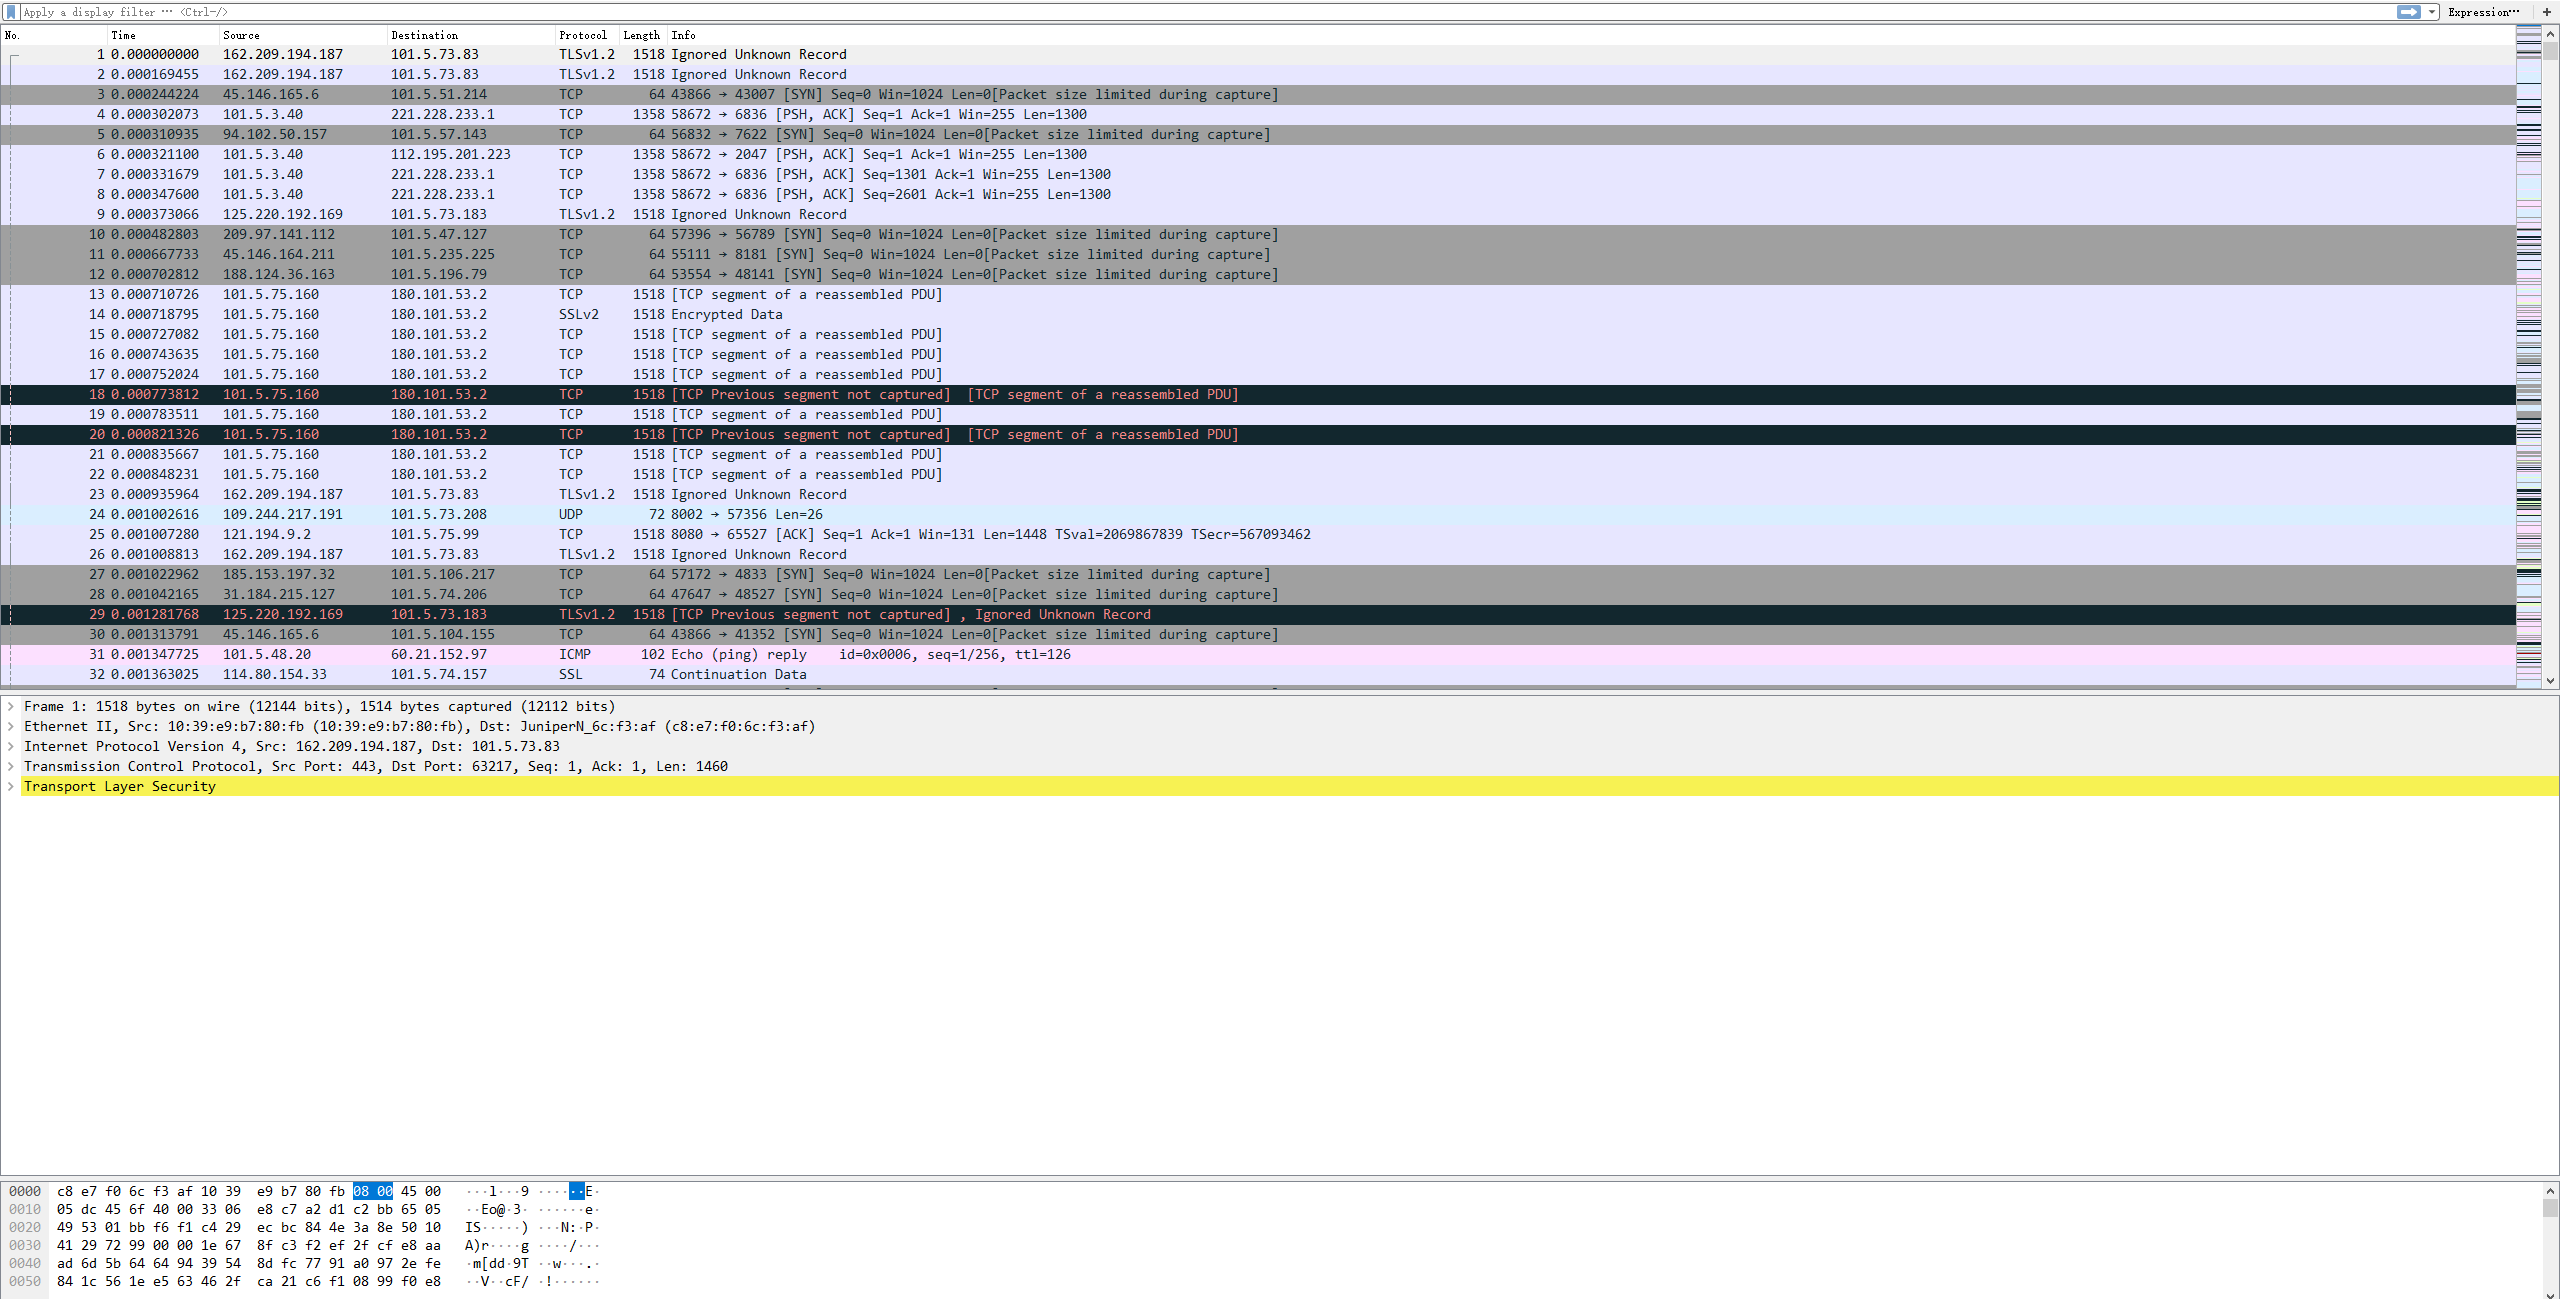
\includegraphics[scale=0.3]{wireshark流量图.png}
    % 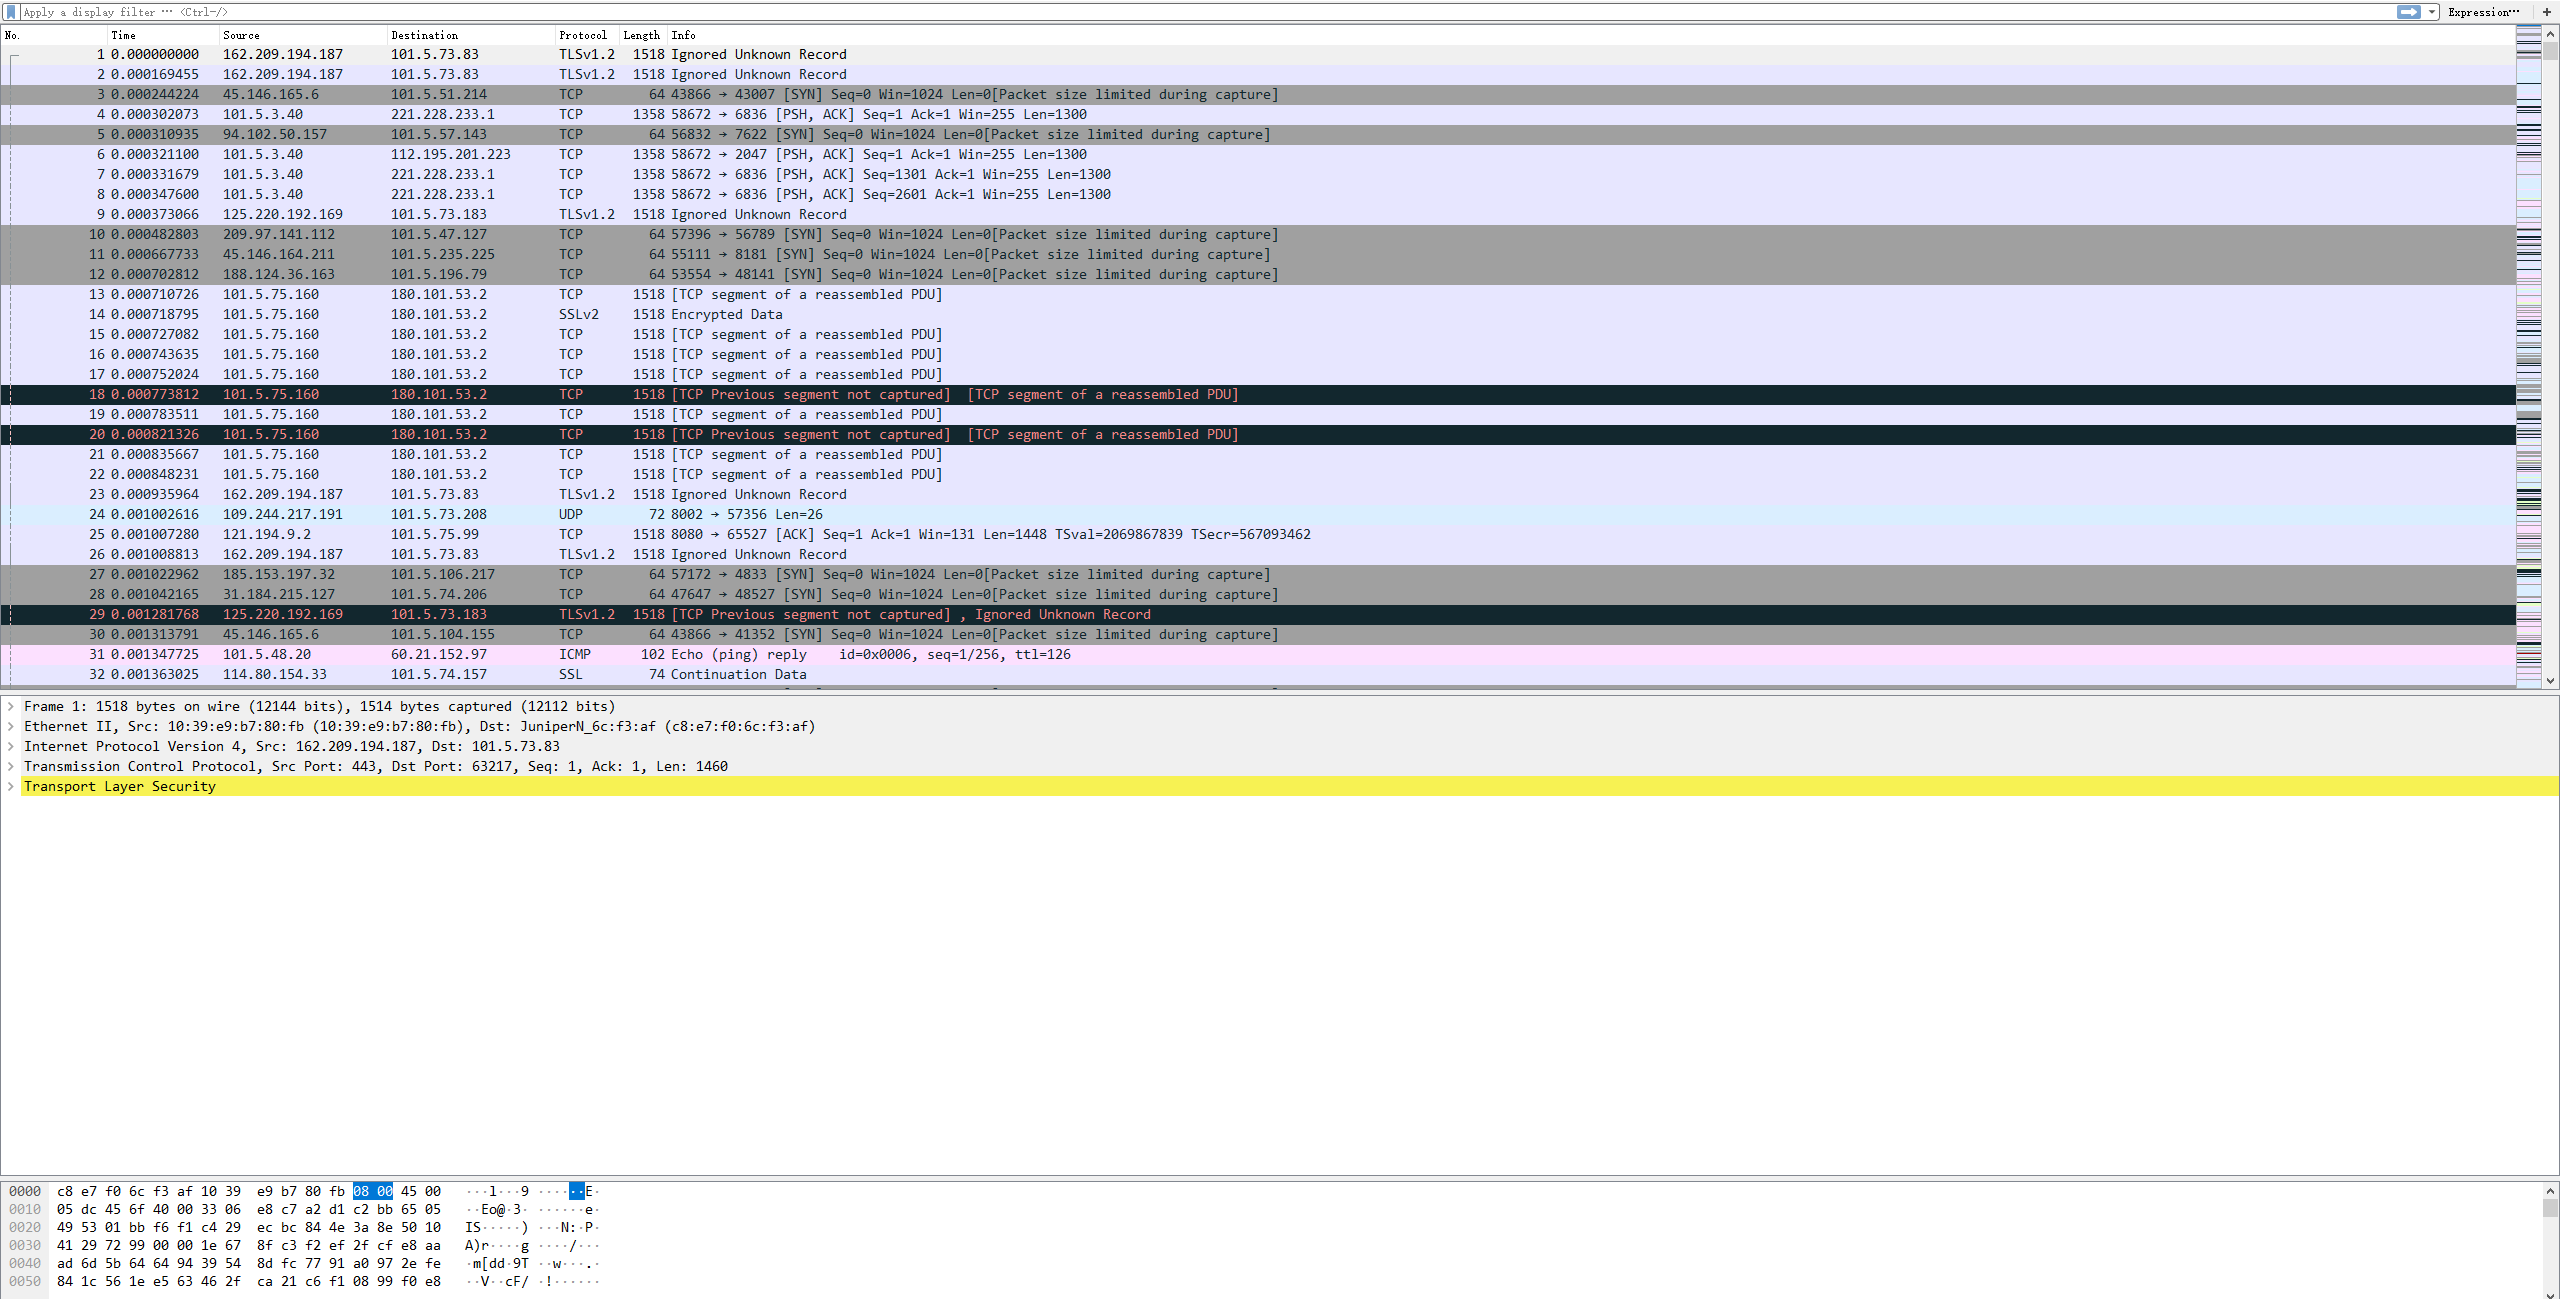
\includegraphics[width=0.6\linewidth]{wireshark流量图.png}
    \caption{流量数据示意图}
    \label{fig:wireshark}
  \end{figure}

% !TeX root = ../thuthesis-example.tex

\chapter{基于图结构的RNN及其网络流量异常检测算法}

\section{引言}
% Recurrent network的应用主要如下两部分:

% 文本相关。主要应用于自然语言处理(NLP)、对话系统、情感分析、机器翻译等等领域,Google翻译用的就是一个7-8层的LSTM模型。
% 时序相关。就是时序预测问题(timeseries),诸如预测天气、温度、包括个人认为根本不可行的但是很多人依旧在做的预测股票价格问题
% 这些问题都有一个共同点,就是有先后顺序的概念的。举个例子: 根据前5天每个小时的温度,来预测接下来1个小时的温度。典型的时序问题,温度是从5天前,一小时一小时的记录到现在的,它们的顺序不能改变,否则含义就发生了变化;再比如情感分析中,判断一个人写的一篇文章或者说的一句话,它是积极地(positive),还是消极的(negative),这个人说的话写的文章,里面每个字都是有顺序的,不能随意改变,否则含义就不同了。

% 全连接网络Fully-Connected Network,或者卷积神经网络Convnet,他们在处理一个sequence(比如一个人写的一条影评),或者一个timeseries of data points(比如连续1个月记录的温度)的时候,他们缺乏记忆。一条影评里的每一个字经过word embedding后,被当成了一个独立的个体输入到网络中;网络不清楚之前的,或者之后的文字是什么。这样的网络,我们称为feedforward network。

% 但是实际情况,我们理解一段文字的信息的时候,每个文字并不是独立的,我们的脑海里也有它的上下文。比如当你看到这段文字的时候,你还记得这篇文章开头表达过一些关于LSTM的信息;

% 所以,我们在脑海里维护一些信息,这些信息随着我们的阅读不断的更新,帮助我们来理解我们所看到的每一个字,每一句话。这就是RNN的做法:维护一些中间状态信息。
% \section{网络流量的时空特性}

% \section{基于图结构的RNN原理}
% 神经网络是目前计算机科学最流行的算法之一,它在图像识别、语音识别和自然语言处理等领域取得了重大突破。卷积神经网络、循环神经网络。
\section{神经网络}

神经网络(Neural Network,NN),又称人工神经网络(Artificial Neural Network,ANN),是20世纪80 年代以来人工智能领域兴起的研究热点。它的定义有很多,其中第一批神经计算机的发明者Robert Hecht-Nielsen博士对神经网络的定义是“ 一个由许多简单的,高度互连的处理元素组成的计算系统, 它们通过对外部输入的动态状态反应来处理信息。或者也可以认为人工神经网络是一种计算模型,它的灵感来自于人脑中生物神经网络处理信息的方式。”
最近十多年来,针对人工神经网络的研究工作已经取得了重大进展,其在模式识别、自动控制、预测估计等领域已成功地解决了许多现代计算机难以解决的实际问题。

\subsection{神经网络的类型}
神经网络有很多类,这些类也有子类,最常用的类有如下几种。
\begin{enumerate}
    \item 前馈神经网络.
前馈神经网络是一种人工神经网络,单元之间的连接不形成循环。在这种网络中,信息只有一个方向,即向前移动,从输入节点,通过隐藏节点(如果有的话),然后到输出节点。网络中不存在循环或环路。
我们可以区分两种类型的前馈神经网络。
\begin{enumerate}
    \item 单层感知器。
    这是最简单的前馈神经网络,不包含任何隐藏层,也就是说它只由单层的输出节点组成。之所以说是单层,是因为我们在计算层数的时候,并不包括输入层,原因是在输入层没有进行计算,输入通过一系列的权重直接反馈给输出。
    \item 多层感知器(MLP)。
这类网络由多层计算单元组成,通常以前馈方式相互连接。一层中的每个神经元都与后一层的神经元有定向连接。在许多应用中,这些网络的单元应用一个sigmoid函数作为激活函数。MLP是非常有用的,一个很好的原因是,它们能够学习非线性表示(大多数情况下,呈现给我们的数据是不可线性分离的。
\item  卷积神经网络(CNN)。
卷积神经网络与普通的神经网络非常相似,它们是由具有可学习权重和偏差的神经元组成的。在卷积神经网络(CNN,或ConvNet或移位不变或空间不变)中,单元连接模式的灵感来自于视觉皮层的组织,单元在一个被称为感受场的受限空间区域内对刺激做出反应。感受场部分重叠,覆盖了整个视场。单元响应可以用卷积运算在数学上近似。它们是多层感知器的变体,使用最少的预处理。它们的广泛应用是在图像和视频识别,推荐系统和自然语言处理。CNNs需要大量的数据来进行训练。
\end{enumerate}
\item  循环神经网络
在循环神经网络(RNN)中,单元之间的连接形成了一个定向循环(它们向前传播数据,同时也向后传播数据,从较后的处理阶段到较早的阶段)。这使得它能够表现出动态的时间行为。与前馈神经网络不同,RNNs可以利用其内部存储器处理任意输入序列。这使得它们适用于未分割、连接的手写识别、语音识别和其他一般序列处理器等任务。
\end{enumerate}


神经网络的灵感来自于人脑生物神经网络的处理方式。
大脑的基本计算单位是神经元。在人类的神经系统中,大约有860亿个神经元,它们与大约$10^{14}$-$10^{15}$的突触相连。神经网络的基本计算单位也是神经元,通常称为节点或单位。它从其他一些节点或外部源接收输入,并计算输出。每个输入都有一个相关的权重(w),该权重是根据其对其他输入的相对重要性分配的。节点对其输入的加权和应用一个函数。
其想法是,突触强度(权重w)是可学习的,并控制影响的强度及其方向:一个神经元对另一个神经元的兴奋性(正权重)或抑制性(负权重)
% 。在基本模型中,树突将信号传到细胞体,在那里它们都会被相加。如果最后的总和超过了某个阈值,神经元就可以开火,沿着轴突发出一个尖峰。在计算模型中,我们假设尖峰的精确时序并不重要,只有发射的频率能传递信息。我们用激活函数(e.x sigmoid函数)来模拟神经元的发射率,它代表沿轴突的尖峰频率。
% 开火 TODO
% 从上面的解释我们可以得出结论,神经网络是由神经元组成的,生物学上神经元是通过突触连接的,信息在突触中流动(出计算模型的权重),当我们训练一个神经网络时,我们希望神经元每当从数据中学习到特定的模式时就开火,我们用激活函数来模拟开火率。

假设一个神经元接收$𝐷$ 个输入$x_1,x_2,...,x_D$令向量$x=[x_1;x_2;...;x_D]$来
表示这组输入, 净输入也叫净活性值
(Net Activation).
并用净输入(Net Input)$z\in \mathbb{R}$表示一个神经元所获得的输入信
号$x$的加权和,

\begin{equation}
\begin{aligned}    
    z &= \sum_{d=1}^D w_d x_d + b \\
      &= w^Tx + b        
\end{aligned}    
\end{equation}

其中$w=[w_1;w_2;...;w_D] \in \mathbb{R}^D$ 是$𝐷$ 维的权重向量,$b\in \mathbb{R}$是偏置。


净输入$𝑧$在经过一个非线性函数$f(\cdot)$后,得到神经元的活性值(Activation,
\begin{equation}
    a = f(z)
\end{equation}
其中非线性函数$f(\cdot)$称为激活函数。

一个人工神经元的结构如图~\ref{fig:神经元}所示:
\begin{figure}
    \centering
    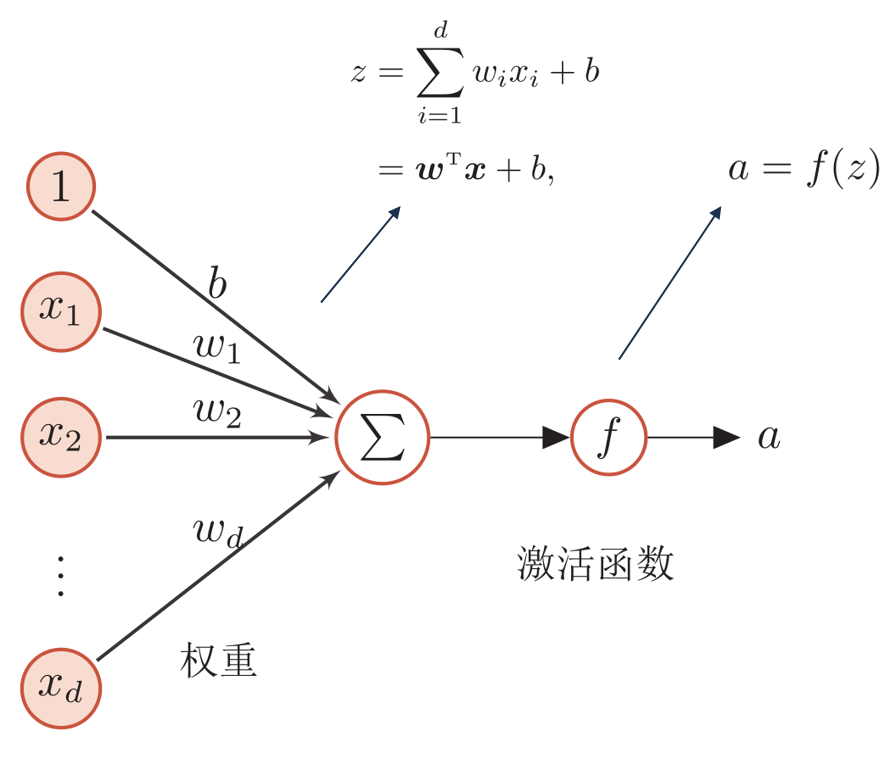
\includegraphics[width=0.6\linewidth]{人工神经元.png}
    \caption{人工神经元模型}
    \label{fig:神经元}
  \end{figure}

在图~\ref{fig:神经元}中,$\vec{x}$为输入向量,$w$和$b$分别是权重和偏移,

神经网络主要由以下几部分组成:
\begin{itemize}
    \item 输入节点(输入层)。在这一层中不进行任何计算,它们只是将信息传递给下一层(大部分时间是隐藏层)。
    \item 隐藏节点(隐藏层)。中间处理或计算在隐藏层中完成的,然后将输入层的权重(信号或信息)传递给下一层(另一个隐藏层或输出层)。一个神经网络也可以不包含隐藏层。
    \item 输出节点(输出层)。它是神经网络的最后一层,接收来自最后一个隐藏层的输入。通过激活函数可以得到合理范围内的理想数值,例如用于分类的softmax函数。
    \item 连接和权重。神经元之间会有边进行连接,每条边会有一定的权重。即每个连接将神经元$i$的输出传递给神经元$j$的输入,每个连接被赋予一个权重$W_{ij}$。
    \item 激活函数。激活函数负责为神经网络引入非线性特征。它把值压缩到一个更小范围,即一个 Sigmoid 激活函数的值区间为 [0,1]。深度学习中有很多激活函数,如Sigmoid、Tanh、ReLU 、Softplus、Softmax 等。下表为常见的激活函数。
    \begin{table}[]
        \caption{激活函数}
        \centering
        \begin{tabular}{|l|l|l|}
        \hline
        名称&表达式&导数\\ \hline
        Sigmoid &  $f(x) = \frac{1}{1+e^{-x}}$ & $f'(x) = f(x)(1-f(x))$
        \\ \hline
        Tanh & $f(x) = \frac{2}{1+e^{-2x}} - 1$ & $f'(x) = 1 - f(x)^2$ \\ \hline
        ReLU & $f(x) = max(0, x)$ & $f(x)=\begin{cases}
        0& \text{x<0}\\
        1& \text{x>=0}
        \end{cases}$ \\ \hline
        Softplus & $f(x) = log(1+e^x)$ & $f'(x) = \frac{1}{1+e^x}$ \\ \hline
        Softmax & $S_i = \frac{e_i}{\sum_j e_j}$ & \\ \hline
        \end{tabular}
        \end{table}
    \item 学习规则。学习规则是一种规则或算法,它修改神经网络的参数,以使网络的给定输入产生一个有利的输出。这个学习过程通常相当于修改权重和阈值。
\end{itemize}

\subsection{RNN}
RNN是一种针对时序数据处理的神经网络模型。相较于普通的神经网络模型来说,更擅长处理序列数据,即该网络其具有短期记忆能力。在循环神经网络中,神经元不但可以接受其他神经元的信息,也可以接受自身的信息,形成具有环路的网络结构。

循环神经网络的通用近似定理[Haykin, 2009]: 如果一个完全
连接的循环神经网络有足够数量的sigmoid 型隐藏神经元,它可以以任意
的准确率去近似任何一个非线性动力系统

% 神经网络有很多类型,这里本文将神经网络划分为前馈神经网络和循环神经网络,其中前馈神经网络包含单层感知机、多层感知机(MLP)、卷积神经网络(CNN)等。
% 本文主要介绍循环神经网络, 循环神经网络(Recurrent Neural Network,RNN)是一类具有短期记忆能力的神经网络。.和前馈神经网络相比,循环神经网络更加符合生物神经网络的结构。
下图~\ref{fig:循环神经网络}是循环神经网络的示意图。
\begin{figure}
    \centering
    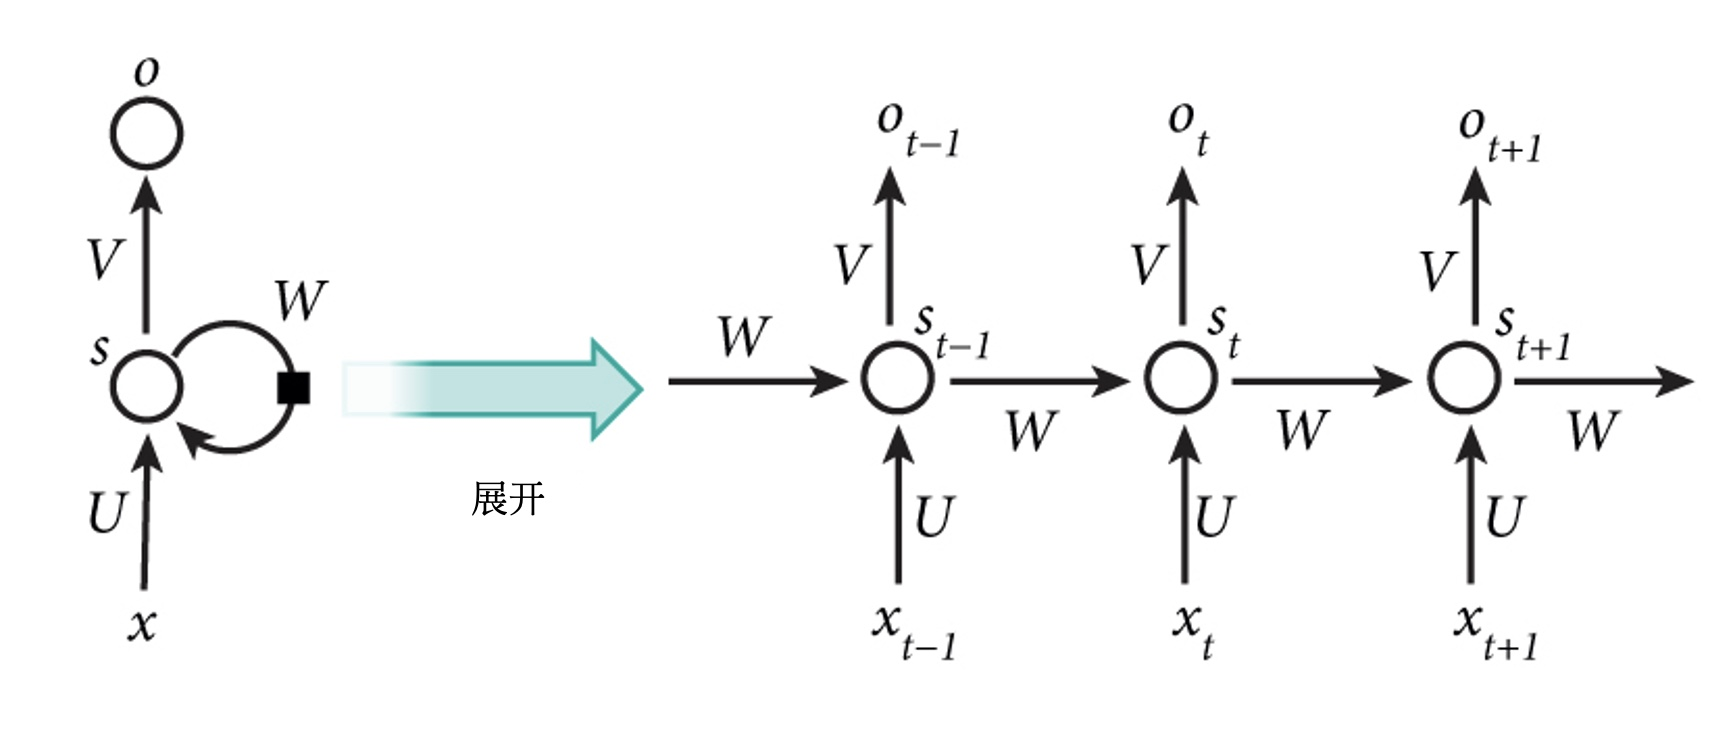
\includegraphics[width=0.6\linewidth]{循环神经网络.jpg}
    \caption{循环神经网络}
    \label{fig:循环神经网络}
  \end{figure}
该图显示了一个循环神经网络被展开成一个完整的神经网络。例如,如果输入序列是一个由5个单词组成的句子,那么网络就会被展开成一个5层神经网络,每个单词一层。这个网络在t时刻接收到输入 $x_t$ 之后,隐藏层的值是 $s_t$ ,输出值是 $o_t$ 。关键一点是, $x_t$ 的值不仅仅取决于 $s_t$ ,还取决于 $s_{t-1}$ 。
  用公式表示如下:
  \begin{equation}
      \begin{aligned}
          O_t &= g(V\cdot S_t) \\
          S_t &= f(U\cdot X_t + W\cdot S_{t-1})
      \end{aligned}
  \end{equation}

  $x_t$表示第$t$步的输入,例如$x_1$表示时刻1的特征向量。$s_t$表示第t步隐藏层状态,也就是网络中的“记忆”。$s_t$是由前一层的隐藏层状态和当前层的输入计算得到。函数$f(\cdot)$通常是一个非线性函数,如tanh或者ReLU。

\subsection{LSTM}
普通RNN有不能处理长依赖的问题,因此Hochreiter提出了一种长短期记忆网络-LSTM,以及它的变种,它是一种特殊的RNN,适用于学习长期依赖。现在LSTM已经被广泛应用于各个领域。

所有RNN都具有链式形式。在普通的RNN中,这种循环是一种非常简单的结构,比如简单的tanh层。
\begin{figure}
    \centering
    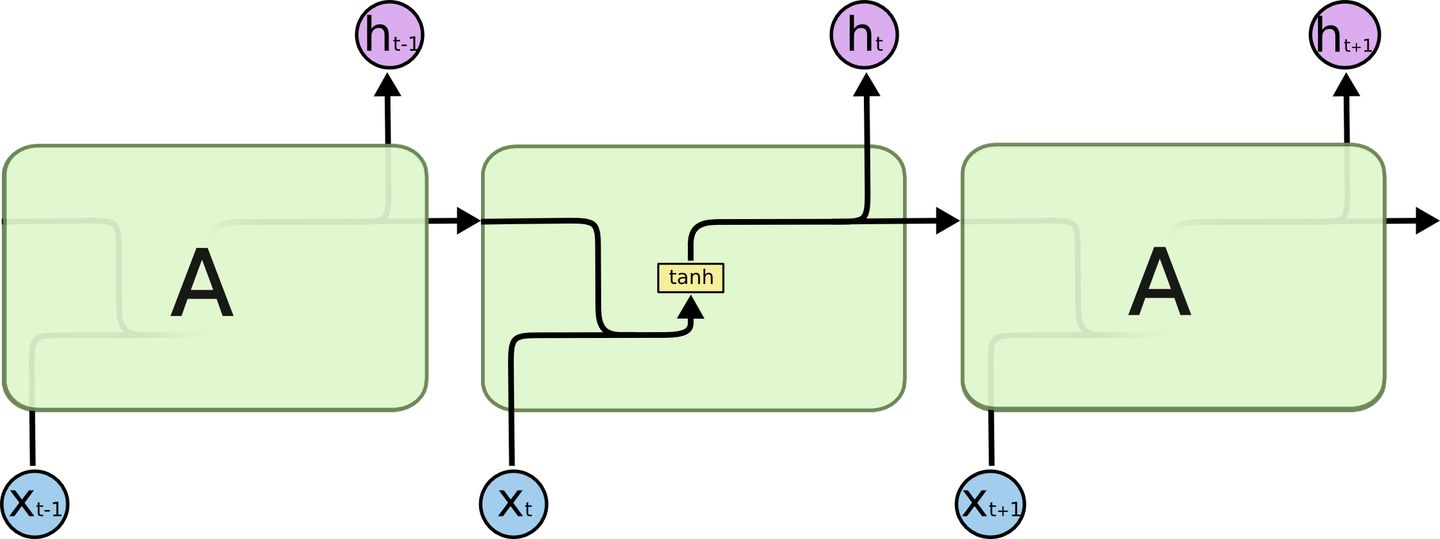
\includegraphics[width=0.6\linewidth]{普通RNN结构.jpg}
    \caption{普通RNN结构}
    \label{fig:普通RNN结构}
  \end{figure}

LSTM也具有这种链式结构,但循环单元里面不再是只有单一的神经网络层,而是构建了一些“门”(Gate)。原来的 RNN,由于这种链式结构的限制,很长的时刻以前的输入对现在的网络影响非常小,后向传播时那些梯度也很难影响很早以前的输入,即会出现梯度消失的问题。而 LSTM 通过构建“门”,让网络能记住那些非常重要的信息,比如遗忘门,来选择性清空过去的记忆和更新较新的信息。
\begin{figure}
    \centering
    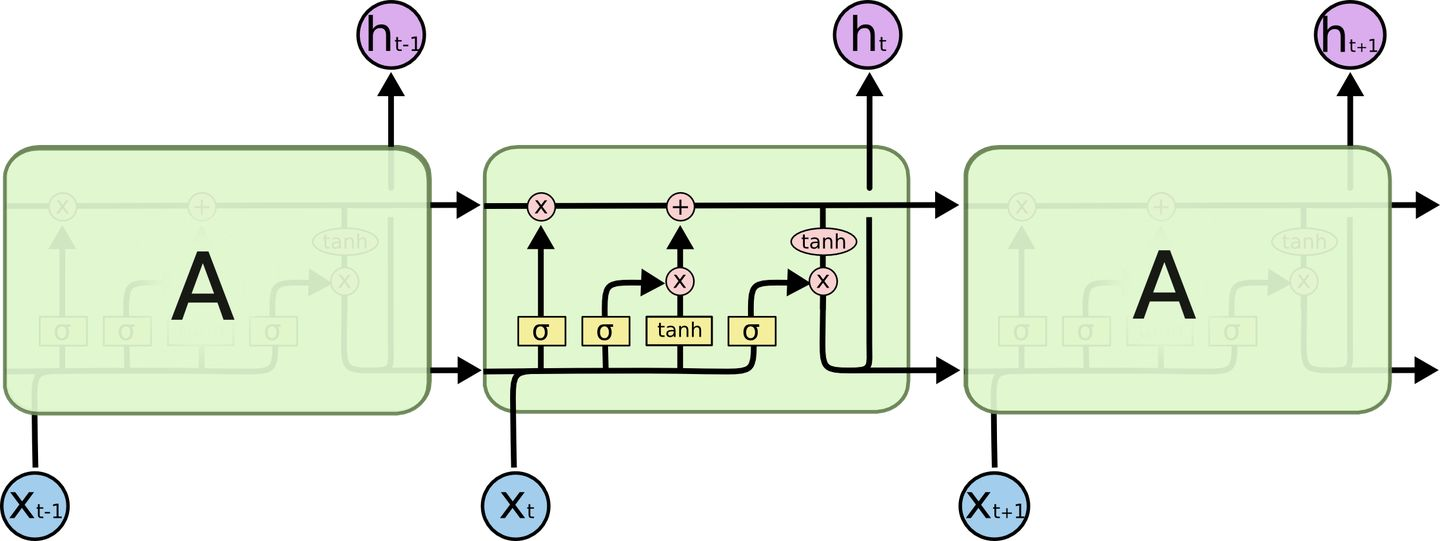
\includegraphics[width=0.6\linewidth]{LSTM结构.jpg}
    \caption{LSTM结构}
    \label{fig:LSTM结构}
  \end{figure}
  LSTM 中的第一步是决定从单元状态中丢弃什么信息。通过加入一个称为忘记门的$\sigma$层完成。遗忘门会读取上一时刻的输出$h_{t-1}$和当前时刻的输入$x_t$,计算出一个维度为n的向量$f_t$,该向量的值均在$(0, 1)$之间。1 表示“完全保留”上个神经元的状态信息,0 表示“完全舍弃”。

\begin{equation}
    \begin{aligned}
        f_t = \sigma(W_f\cdot x_t + U_f\cdot h_{t-1} + b_f)
    \end{aligned}
\end{equation}

下一步是确定该神经元的哪些新状态信息被存放在单元状态中。这里包含两个部分。第一,sigmoid 层,即 “输入门层” ,决定LSTM单元将更新哪些值。然后, tanh 层创建一个新的候选值$z_t$的向量,该向量可以加入到下一层单元状态中。

\begin{equation}
    \begin{aligned}
        i_t = \sigma(W_i\cdot[h_{t-1},x_t] + b_i)
    \end{aligned}
\end{equation}

\begin{equation}
    \begin{aligned}
        \widetilde {C_t} = tanh(W_C\cdot[h_{t-1},x_t]+b_C)
    \end{aligned}
\end{equation}
最后一步是将旧单元状态$c_{t-1}$更新为新状态$c_t$。把旧状态与遗忘门$f_t$相乘,丢弃掉之前需要丢弃的信息。接着与新状态进行相加。综合得出该神经元的输出的状态,也即更新单元的状态。
\begin{equation}
    \begin{aligned}
        C_t = f_t * C_{t-1} + i_t * \widetilde{C_t}
    \end{aligned}
\end{equation}

\subsection{GRU}
循环门单元(Gated Recurrent Unit,GRU),由 Cho, et al. (2014)提出。它组合了遗忘门和输入门到一个单独的“更新门”中。它也合并了cell state和hidden state,并且做了一些其他的改变。结果模型比标准LSTM模型更简单,
\begin{figure}
    \centering
    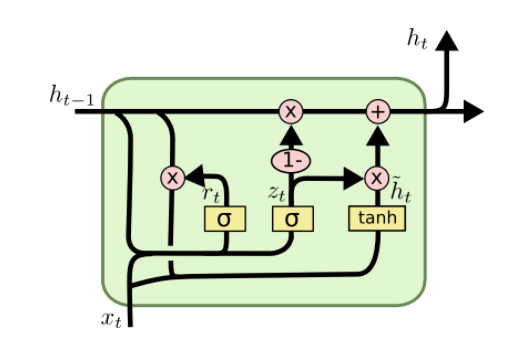
\includegraphics[width=0.6\linewidth]{GRU结构.png}
    \caption{GRU结构}
    \label{fig:GRU结构}
  \end{figure}

  \begin{equation}
    \begin{aligned}
        z_t = \sigma(W_z\cdot [h_{t-1},x_t])
    \end{aligned}
\end{equation}

\begin{equation}
    \begin{aligned}
        r_t = \sigma(W_r\cdot[h_{t-1},x_t])
    \end{aligned}
\end{equation}

\begin{equation}
    \begin{aligned}
        \widetilde {h_t} = tanh(W\cdot[r_t * h_{t-1}, x_t])
    \end{aligned}
\end{equation}

\begin{equation}
    \begin{aligned}
        h_t = (1- z_t) * h_{t-1} + z_t * \widetilde{h_t}
    \end{aligned}
\end{equation}
由图中结构可以看出,GRU是通过一个循环神经网络和“门”机制来不断更新内部参数,GRU算法的伪代码如下表所示。

\begin{algorithm}[!h]
    \caption{\emph{GRU}}
    \label{alg}
    \begin{algorithmic}[1]
      \Require
        t

      \Ensure
        内部参数
      \State 初始化t时刻单元状态
      \For{t $\leftarrow$ $1$ to $T$}
        $output_t$ = t
        $state_t$ = $output_t$
      \EndFor
    % %   \While {$\mathcal{L}$没有收敛}
    %       \State 利用公式 计算每一个节点$v$的$q_\phi(\bm{y}_v | \bm{A}, \bm{X}, Y_L)$以及$h_v^{K-1}$
    %       \For{i $\leftarrow$ $1$ to $m$}
    %       \State 从分布$q_\phi(Y_U | \bm{A}, \bm{X}, Y_L)$中采样$Y_U$
    %       \State 在采样得到的$Y_U$基础上,利用公式计算$q_\phi(\bm{z}| \bm{A}, \bm{X}, Y)$ 
    %        \For{j $\leftarrow$ $1$ to $n$}
    %        \State 从分布$q_\phi(\bm{z}| \bm{A}, \bm{X}, Y)$ 中采样$\bm{z}$
    %        \State 在采样得到的$\bm{z}$基础上用公式 计算$p_{\theta}(\bm{y}_v|\bm{A}, \bm{X}, \bm{z})$
    %        \EndFor
    %       \EndFor
    %       \State 用公式计算目标函数$\mathcal{L}(\theta, \phi)$ 
    %       \State 用梯度下降法更新$q_{net1}$,$q_{net2}$和$p_{net}$的所有参数
    %   \EndWhile
      %\State \Return $P_{net}$
    \end{algorithmic}
  \end{algorithm}

\begin{algorithm}[!h]
    \caption{\emph{LSTM层}}
    \begin{algorithmic}[1]
        \Require 一组按时间排列的向量组
        \Ensure 按时间排列的向量组
        \State $\vec C_0 = \vec 0$
        \State $\vec h_0 = \vec 0$
        \For{$t$ \leftarrow $1$ to $T$}


        \EndFor
    \end{algorithmic}
\end{algorithm}
  
$  state_t = 0
  for input_t in input_sequence:
    output_t = activation(dot(W, input_t) + dot(U, state_t) + b)
    state_t = output_t$
\section{基于图结构的RNN}
有向权重图$G=(V,E,W)$,$V$表示特征节点的集合,其中$|V|=N$, $E$表示特征间的关联关系,即图中的边,$W∈R[N*N]$为特征节点的相似度的加权邻接矩阵。将流量表示为G的一个图信号,P为每个节点特征数,则-时间t观察到的图信号。那么流量预测目的就是:给定G下,学得一个函数将T'个历史图信号映射到未来T时刻的图信号:
\begin{equation}
    h[X^{t-T+1}, X^{t-T+2},...,X^{t}; G] \Rightarrow [X^{t+1}, X^{t+2}, ..., X^{t+T}]
\end{equation}

\begin{equation}
    r^{(t)} = \sigma(\Theta_r\star G[X^{(t)},H^{t-1}] + b_r)
\end{equation}

\begin{equation}
    u^{(t)} = \sigma(\Theta_u\star G[X^{(t)},H^{t-1}] + b_u)
\end{equation}

\begin{equation}
    C^{(t)} = tanh(\Theta_C\star_G[X^{(t)},(r^{(t)}\odot H^{(t-1)})] + b_c)
\end{equation}

\begin{equation}
    H^{(t)} = u^{(t)}\odot H^{(t-1)} + (1 - u^{(t)}) \odot C^{(t)}
\end{equation}

其中$X^{(t)}$, $H^{(t)}$表示在时间 $t$ 的输入和输出,$r^{(t)}$ $u^{(t)}$分别是在时间 $t$的复位门和更新门。$\star_G$  表示在等式 2 中定义的扩散卷积,并且  是对应滤波器的参数。与GRU相似,DCGRU可用于构建递归神经网络层,并使用反向传播进行训练。

我们利用递归神经网络(RNN)对时间依赖性进行建模。特别是,我们使用门控循环单元(GRU)(Chung等,2014),它是RNN的简单而强大的变体。我们用扩散卷积代替了GRU中的矩阵乘法,这导致了我们提出的扩散卷积门控递归单元(DCGRU)。

\subsection{aa}
通常,计算卷积会很费时。 但是,如果$G$稀疏,则可以使用总时间复杂度 $O(K \mid \varepsilon \mid \ll O(N^ 2)$ 递归稀疏矩阵乘法来有效地计算方程2。


% 循环神经网络解决了这个问题。它们是带有循环的网络,允许信息持续存在。循环神经网络可以被认为是同一个网络的多个副本,每个副本都会向后继者传递信息。
\section{实验方案设计及实验流程}
\begin{equation*} hl=[hl_{1},\ hl_{2},\ \ldots,\ hl_{n-f+1}] \tag{-} \end{equation*}

\section{算法性能评估}

其中多分类任务的准确率指标为对于每个标签,分别计算precision,然后取不加权平均。$\mathbb{E}$

\begin{table*}[t]
    \small
    \caption{部分评估结果,待填充具体数值}
    \label{table2}
    \centering
    \begin{tabular}{c|c|ccc|ccc|cc}
    \toprule
    
     数据集 &  任务  &  
     LR &  NB & DT & CNN & CNN-LSTM & GRU & DCRNN-A & DCRNN-B \\
    \midrule
    % & 5\% & 79.87 & 80.61 & 79.08 & 81.69 & 78.05 & 75.80 & 82.21 & \textbf{82.49}\\
    
    % & 4\% &79.35 & 80.22 & 78.89 & 80.85 & 75.07 & 72.41 & 82.11 & \textbf{82.44} \\
    
    UNSW-NB15 & 二分类 & 0.848 & 79.33 & 78.52 &  80.51 & 62.74 & 68.91 & \textbf{82.69} & 81.66 \\ 
    
    & 多分类 &76.73 & 77.96 & 76.82 & 77.98 & 47.11 & 56.30 & \textbf{81.05} & 79.94 \\
    
    % & 1\% & 66.58 & 70.09 & 68.18 & 71.23 & 32.95 & 46.71 & \textbf{71.76} & 71.62 \\
    \midrule
    % & 5\%& 70.55 & 69.41 & 68.40 &  71.45 & 70.72 & 65.11 & 71.24 &  \textbf{71.89} \\
    % & 4\% & 69.11 & 68.33& 67.13 & 70.37 & 70.41 & 64.61 & 69.74 & \textbf{71.10} \\
    NSL-KDD & 二分类 & 68.26 & 67.11 & 65.54 & 70.18 & 65.04 & 58.49 & 70.26 & \textbf{70.88} \\
    & 多分类 & 67.01 & 67.37 & 66.41 & 68.31 & 56.16 & 53.18 & 68.47 & \textbf{70.24} \\
    % & 1\% & 60.08 & 61.39 & 61.25 & 63.25 & 30.28 & 49.57 & 62.21 & \textbf{64.91} \\
    \midrule
    % & 0.5\%& 82.18 & 80.01 & 81.32 &  78.25 & \textbf{82.73} & 78.97 & 82.17 & 80.70\\
    % & 0.4\%& 80.85 & 79.09 & 79.82 & 76.32 & 81.53 &  75.86 & \textbf{81.70} & 79.92\\
    CAMPUS & 二分类 & 79.98 & 77.95 & 79.51 & 75.62 & 79.80 & 75.25 & \textbf{80.69} & 79.10\\
    & 多分类 & 76.33 & 77.01 & 77.54 & 73.01 & 76.59 & 59.28 & 78.12 & \textbf{78.89}\\
    % & 0.1\% & 69.21 & 70.99 & 71.42 & 67.92 & 42.46 & 55.92 & 72.23 & \textbf{73.17}\\
    
     \bottomrule
    
    \end{tabular}
    \end{table*}

\subsection{基于开源数据集的检测结果}
% \begin{algorithm}
%     \caption{A}
%     \label{alg:A}
%     % \begin{algorithmic}
%     \STATE {set $r(t)=x(t)$} 
%     \REPEAT 
%     \STATE set $h(t)=r(t)$ 
%     \REPEAT
%     \STATE set $h(t)=r(t)$ 
%     \UNTIL{B} 
%     \UNTIL{B}
%     % \end{algorithmic}
%     \end{algorithm}
\begin{algorithm}[!h]
    \caption{\emph{GRNN}}
    \label{alg}
    \begin{algorithmic}[1]
      \Require
        一组按时间排序的向量组$\vec{x_1}$,$\vec{x_2}$,...,$\vec{x_T}$, 特征间关系图$G$以及它的邻接矩阵$W$

      \Ensure
        按时间排序的向量组$\vec{h_1}$,$\vec{h_2}$,...,$\vec{h_T}$
      \State 通过Xavier方法初始化$q_{net1}$, $q_{net2}$ and $p_{net}$的所有参数
      \While {$\mathcal{L}$没有收敛}
          \State 利用公式 计算每一个节点$v$的$q_\phi(\bm{y}_v | \bm{A}, \bm{X}, Y_L)$以及$h_v^{K-1}$
          \For{i $\leftarrow$ $1$ to $m$}
          \State 从分布$q_\phi(Y_U | \bm{A}, \bm{X}, Y_L)$中采样$Y_U$
          \State 在采样得到的$Y_U$基础上,利用公式计算$q_\phi(\bm{z}| \bm{A}, \bm{X}, Y)$ 
           \For{j $\leftarrow$ $1$ to $n$}
           \State 从分布$q_\phi(\bm{z}| \bm{A}, \bm{X}, Y)$ 中采样$\bm{z}$
           \State 在采样得到的$\bm{z}$基础上用公式 计算$p_{\theta}(\bm{y}_v|\bm{A}, \bm{X}, \bm{z})$
           \EndFor
          \EndFor
          \State 用公式计算目标函数$\mathcal{L}(\theta, \phi)$ 
          \State 用梯度下降法更新$q_{net1}$,$q_{net2}$和$p_{net}$的所有参数
      \EndWhile
      %\State \Return $P_{net}$
    \end{algorithmic}
  \end{algorithm}




%   \begin{algorithm}[!h]
%     \caption{\emph{GSNN}}
%     \label{alg}
%     \begin{algorithmic}[1]
%       \Require
%         图$G$以及它的邻接矩阵$A$,节点特征矩阵$X$以及已知节点的标签信息$T_L$,采样得到的$Y_U$和$\bm{z}$的数量:$m$和$n$

%       \Ensure
%         优化后的$q_{net1}$, $q_{net2}$和$p_{net}$所有参数
%       \State 通过Xavier方法\cite{glorot2010understanding}初始化$q_{net1}$, $q_{net2}$ and $p_{net}$的所有参数
%       \While {$\mathcal{L}$没有收敛}
%           \State 利用公式 \ref{seven} 计算每一个节点$v$的$q_\phi(\bm{y}_v | \bm{A}, \bm{X}, Y_L)$以及$h_v^{K-1}$
%           \For{i $\leftarrow$ $1$ to $m$}
%           \State 从分布$q_\phi(Y_U | \bm{A}, \bm{X}, Y_L)$中采样$Y_U$
%           \State 在采样得到的$Y_U$基础上,利用公式 \ref{eight}计算$q_\phi(\bm{z}| \bm{A}, \bm{X}, Y)$ 
%            \For{j $\leftarrow$ $1$ to $n$}
%            \State 从分布$q_\phi(\bm{z}| \bm{A}, \bm{X}, Y)$ 中采样$\bm{z}$
%            \State 在采样得到的$\bm{z}$基础上用公式\ref{nine} 计算$p_{\theta}(\bm{y}_v|\bm{A}, \bm{X}, \bm{z})$
%            \EndFor
%           \EndFor
%           \State 用公式\ref{ten}计算目标函数$\mathcal{L}(\theta, \phi)$ 
%           \State 用梯度下降法更新$q_{net1}$,$q_{net2}$和$p_{net}$的所有参数
%       \EndWhile
%       %\State \Return $P_{net}$
%     \end{algorithmic}
%   \end{algorithm}

\subsection{基于真实数据的检测结果}
交叉熵损失函数经常用于分类问题中,特别是在神经网络做分类问题时,也经常使用交叉熵作为损失函数,此外,由于交叉熵涉及到计算每个类别的概率,所以交叉熵几乎每次都和sigmoid(或softmax)函数一起出现。

我们用神经网络最后一层输出的情况,来看一眼整个模型预测、获得损失和学习的流程:

神经网络最后一层得到每个类别的得分scores;
该得分经过sigmoid(或softmax)函数获得概率输出;
模型预测的类别概率输出与真实类别的one hot形式进行交叉熵损失函数的计算。

\chapter{流量检测系统的设计与实现}
本文实现的流量异常检测系统按照功能需求可以分为三个模块:数据采集和分析模块,异常检测模块,终端预警模块。

\begin{figure}
    \centering
    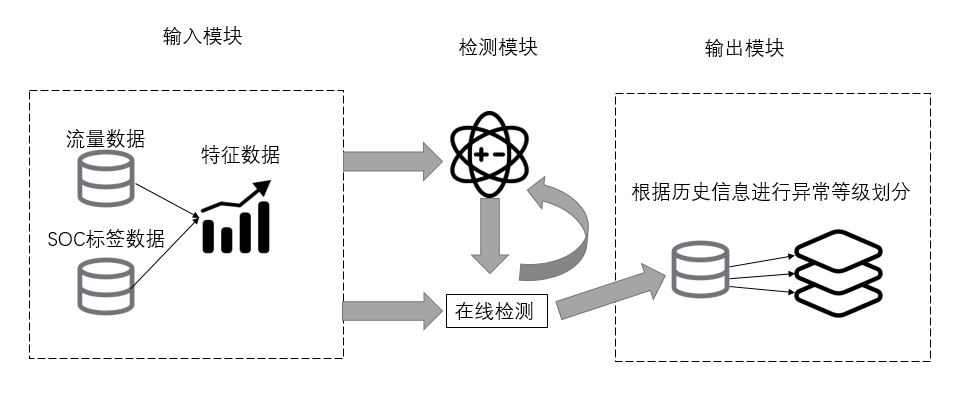
\includegraphics[scale=0.6]{系统架构图.png}
    % 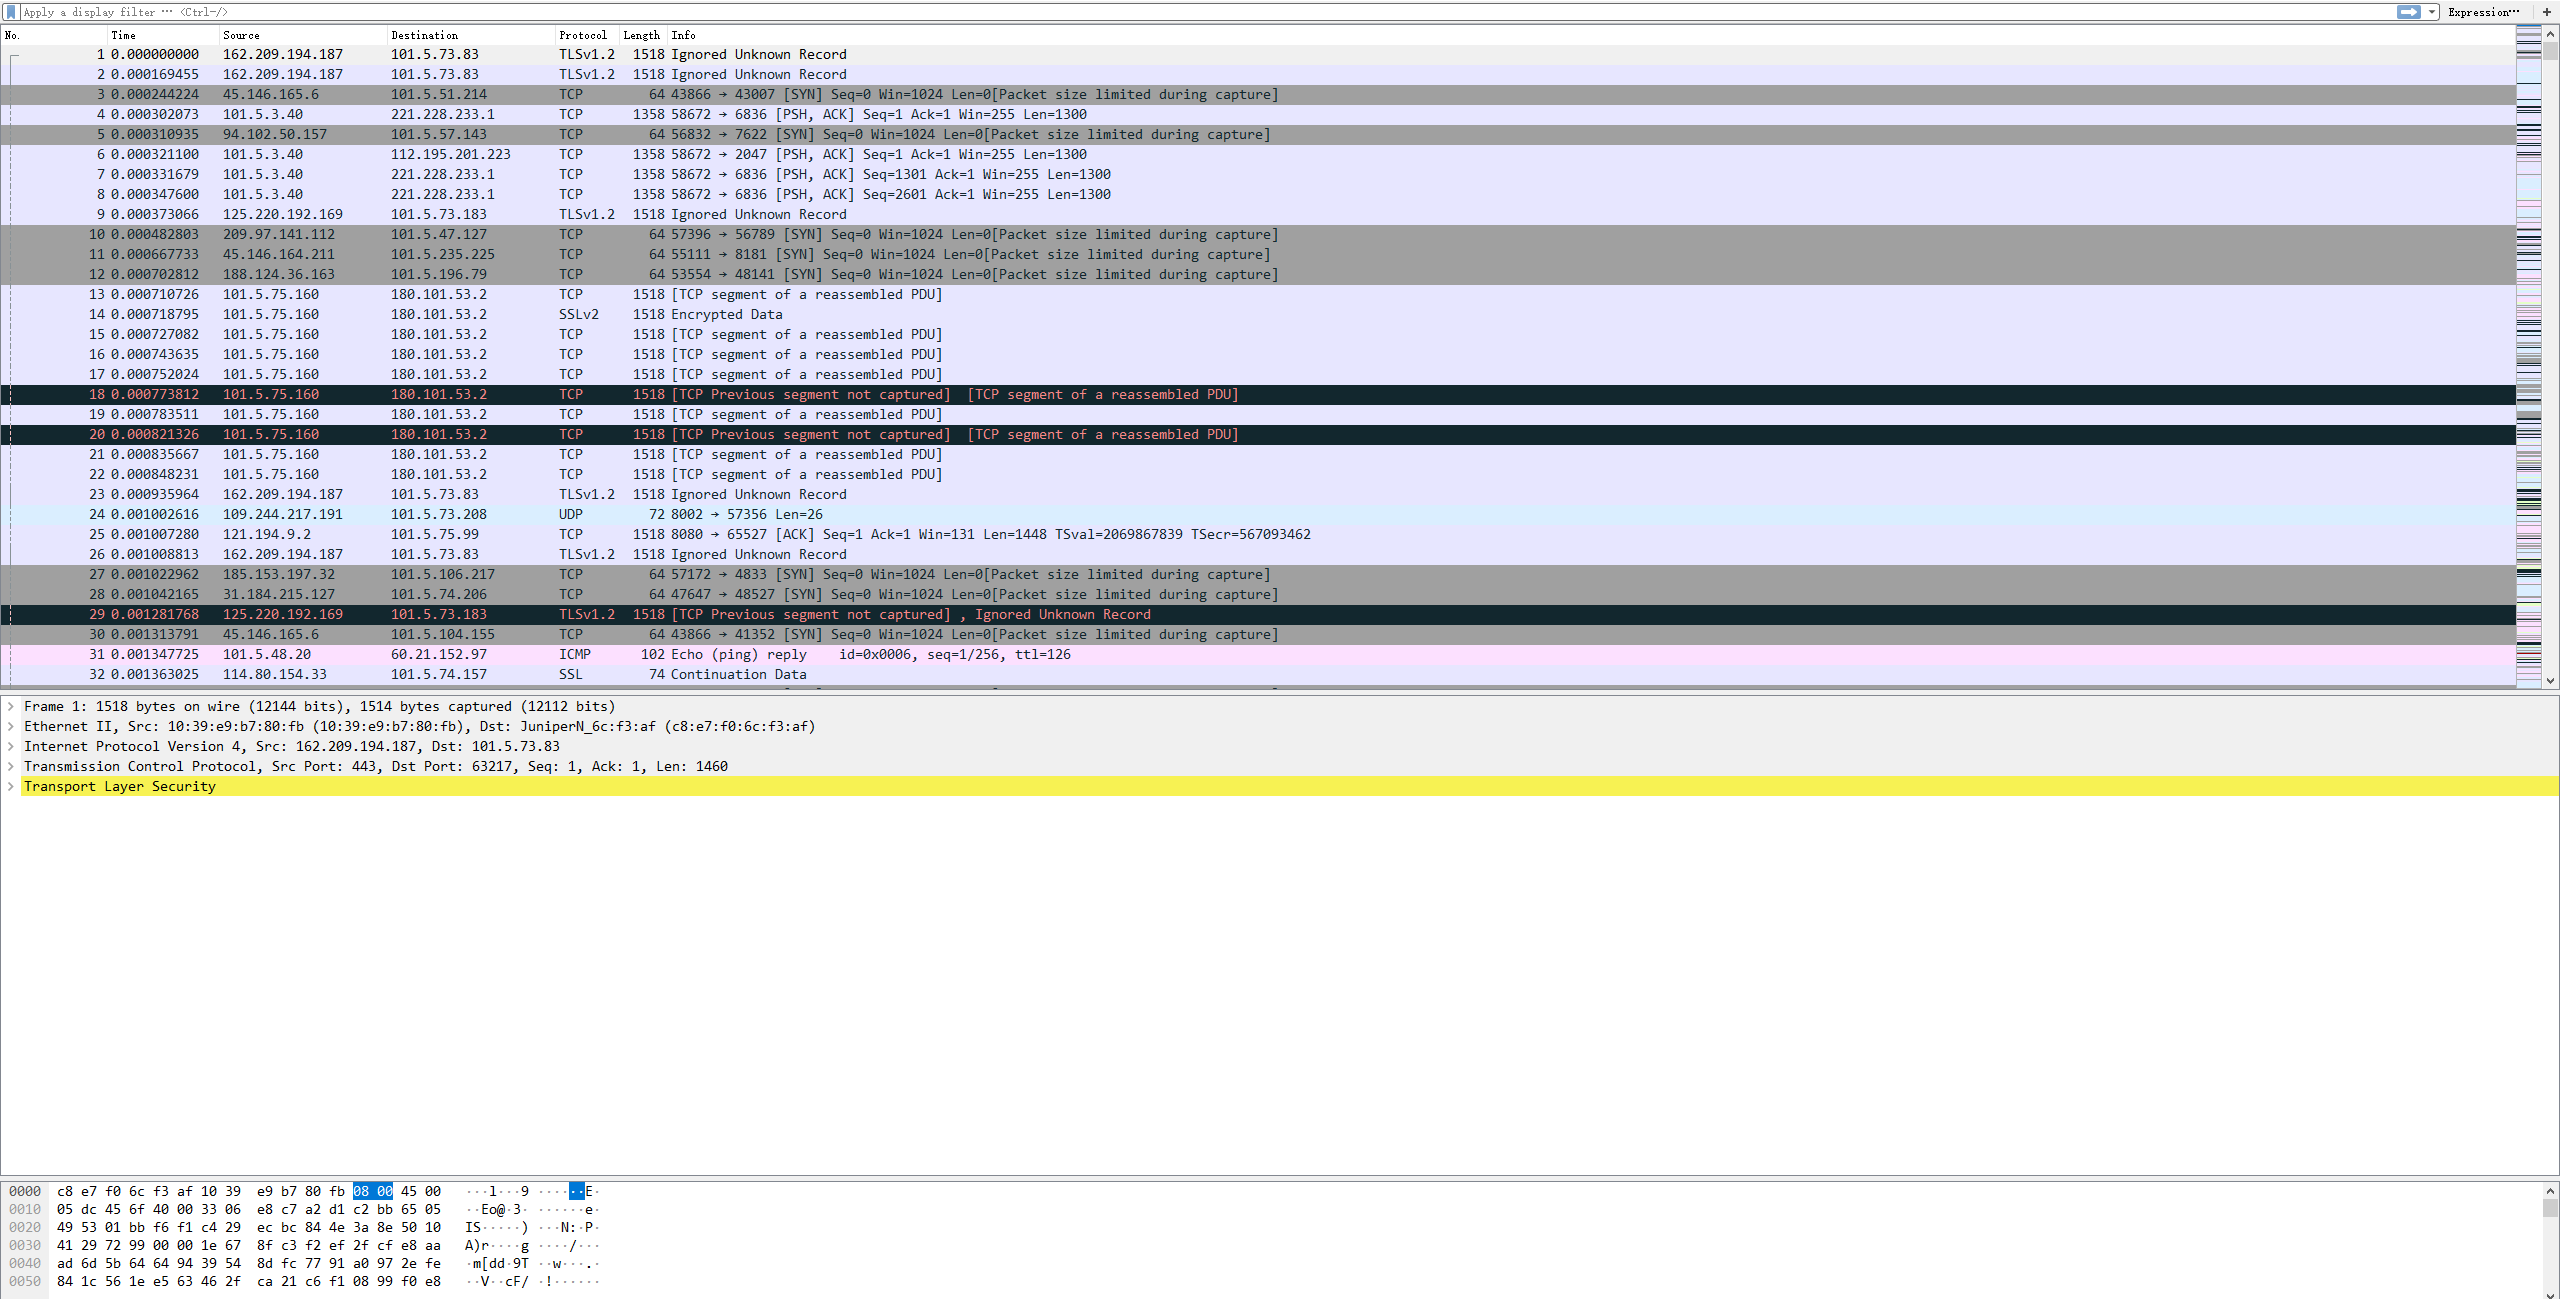
\includegraphics[width=0.6\linewidth]{wireshark流量图.png}
    \caption{系统架构图}
    \label{fig:arch}
  \end{figure}

\section{引言}
下面是对各个模块的介绍:

待补充。

% \section{使用大数据平台应对大规模流量的必要性}
\section{spark 平台介绍}
Spark 是 UC Berkeley AMP Lab 开源的通用分布式并行计算框架,目前已成为 Apache 软件基金会的顶级开源项目。Spark 支持多种编程语言,包括 Java、Python、R 和 Scala,同时 Spark 也支持 Hadoop 的底层存储系统 HDFS,但 Spark 不依赖 Hadoop。

Spark 基于 Hadoop MapReduce 算法实现的分布式计算,拥有 Hadoop MapReduce 所具有的优点,并且具有更高的运算速度。Spark 能够比 Hadoop 运算更快,主要原因是:Hadoop 在一次 MapReduce 运算之后,会将数据的运算结果从内存写入到磁盘中,第二次 MapReduce 运算时在从磁盘中读取数据,两次对磁盘的操作,增加了多余的 IO 消耗;而 Spark 则是将数据一直缓存在内存中,运算时直接从内存读取数据,只有在必要时,才将部分数据写入到磁盘中。除此之外,Spark 使用最先进的 DAG(Directed Acyclic Graph,有向无环图)调度程序、查询优化器和物理执行引擎,在处理批量处理以及处理流数据时具有较高的性能。按照Spark 官网的说法,Spark 相对于 Hadoop 而言,Spark 能够达到 100 倍以上的运行负载。

Spark Core是 Spark 的核心,主要负责任务调度等管理功能。Spark
Core 的实现依赖于 RDDs(Resilient Distributed Datasets,
弹性分布式数据集)的程序抽象概念。

Spark Streaming:这个模块主要是对流数据的处理,支持流数据的可伸缩和容错处理,可以与 Flume(针对数据日志进行优化的一个系统)和 Kafka(针对分布式消息传递进行优化的流处理平台)等已建立的数据源集成。Spark Streaming 的实现,也使用 RDD 抽象的概念,使得在为流数据(如批量历史日志数据)编写应用程序时,能够更灵活,也更容易实现。

Spark 有多种运行模式, Spark 支持本地运行模式(Local 模式)、独立运行模式(Standalone 模式)、Mesos、YARN(Yet Another Resource Negotiator)、Kubernetes 模式等。

本地运行模式是 Spark 中最简单的一种模式,也可称作伪分布式模式。本文中的系统就是使用的本地运行模式。

独立运行模式为 Spark 自带的一种集群管理模式,Mesos 及 YARN 两种模式也是比较常用的集群管理模式。相比较 Mesos 及 YARN 两种模式而言,独立运行模式是最简单,也最容易部署的一种集群运行模式。


Spark 底层还支持多种数据源,能够从其它文件系统读取数据,如 HDFS、Amazon S3、Hypertable、HBase 等。Spark 对这些文件系统的支持,同时也丰富了整个 Spark 生态的运行环境。

Spark 支持多种分布式部署模式,主要支持三种部署模式,分别是:Standalone、Spark on YARN和 Spark on Mesos模式。

Standalone模式为 Spark 自带的一种集群管理模式,即独立模式,自带完整的服务,可单独部署到一个集群中,无需依赖任何其他资源管理系统。它是 Spark 实现的资源调度框架,其主要的节点有 Driver 节点、Master 节点和 Worker 节点。Standalone模式也是最简单最容易部署的一种模式。

Spark on YARN模式,即 Spark 运行在Hadoop YARN框架之上的一种模式。Hadoop YARN(Yet Another Resource
Negotiator,另一种资源协调者)是一种新的 Hadoop 资源管理器,它是一个通用资源管理系统,可为上层应用提供统一的资源管理和调度。

Spark on Mesos模式,即 Spark 运行在Apache Mesos框架之上的一种模式。Apache Mesos是一个更强大的分布式资源管理框架,负责集群资源的分配,它允许多种不同的框架部署在其上,包括YARN。它被称为是分布式系统的内核。

三种架构都采用了Master/Worker(Slave)的架构,Spark 分布式运行架构大致如下:
\begin{figure}
    \centering
    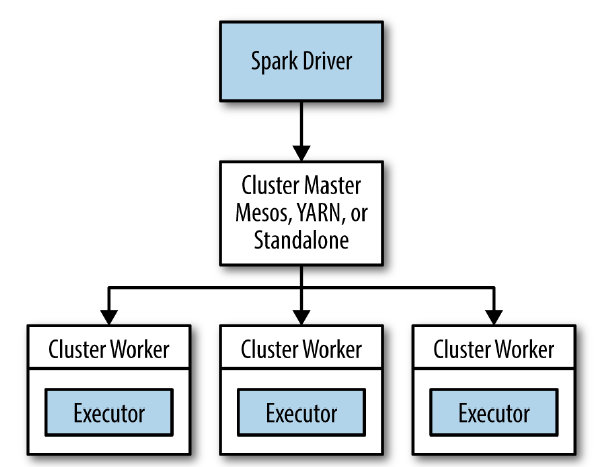
\includegraphics[scale=0.6]{spark分布式运行架构.jpg}
    % 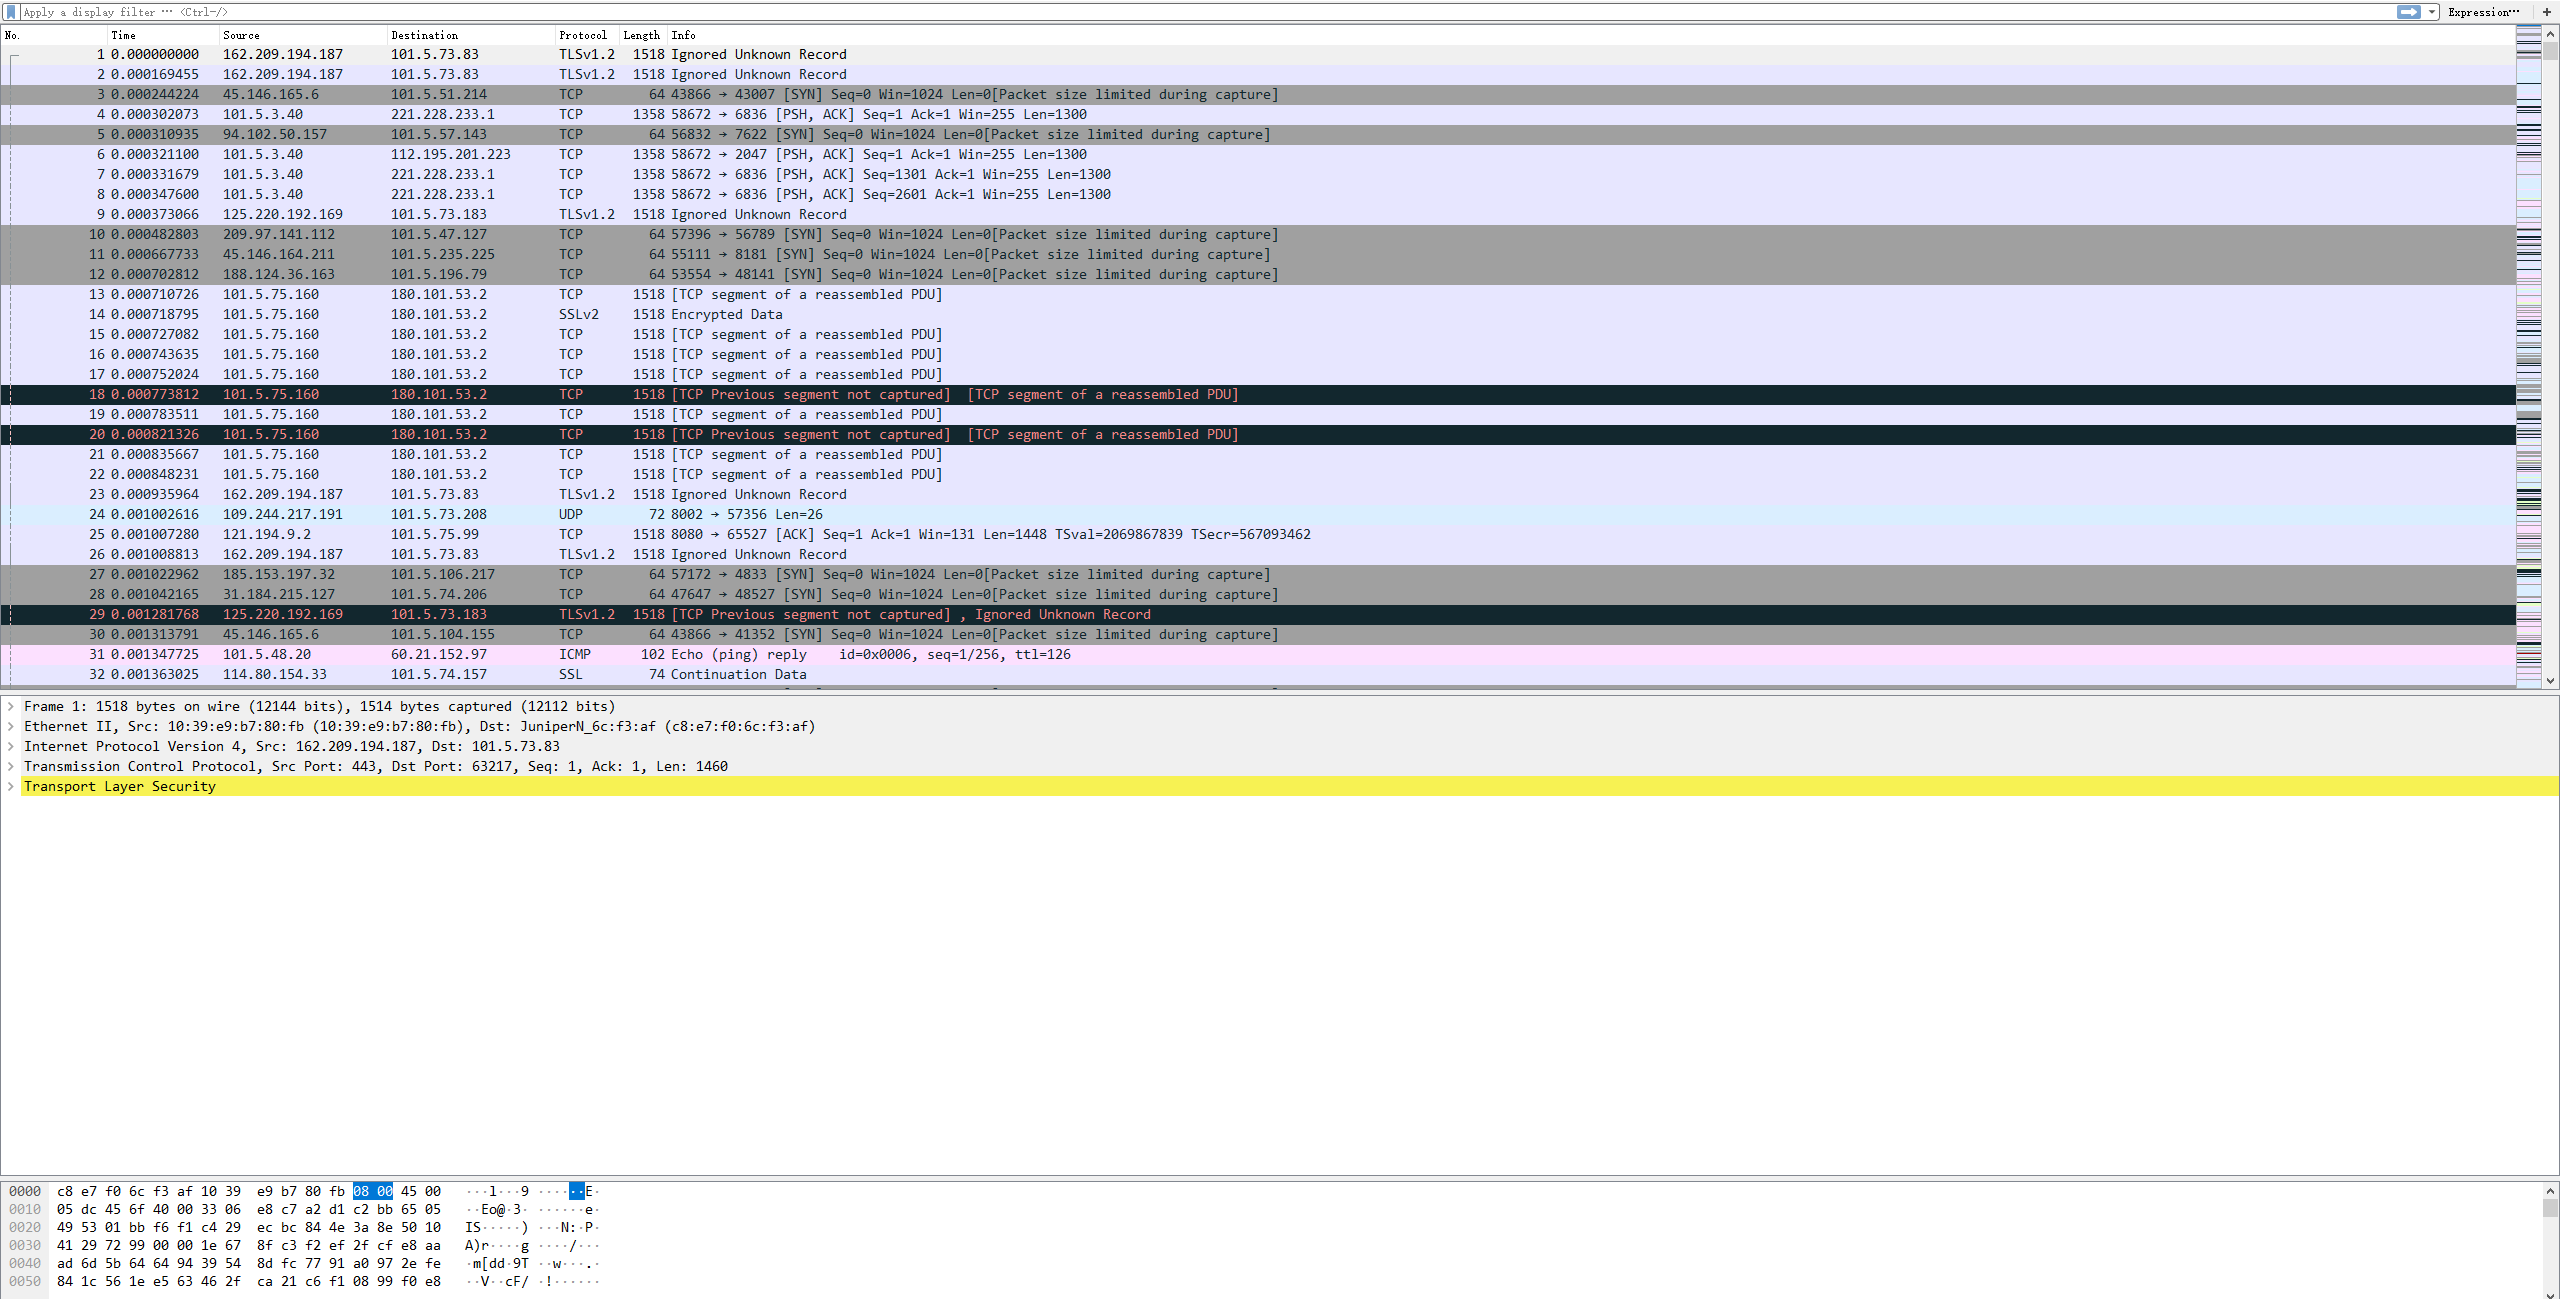
\includegraphics[width=0.6\linewidth]{wireshark流量图.png}
    \caption{spark分布式运行架构}
    \label{fig:spark}
  \end{figure}

  运行一个Spark Streaming应用程序,有下面一些步骤

  有管理器的集群-这是任何Spark应用程序都需要的需求,详见部署指南
  将应用程序打为jar包-你必须编译你的应用程序为jar包。如果你用spark-submit启动应用程序,你不需要将Spark和Spark Streaming打包进这个jar包。如果你的应用程序用到了高级源(如kafka,flume),你需要将它们关联的外部artifact以及它们的依赖打包进需要部署的应用程序jar包中。例如,一个应用程序用到了TwitterUtils,那么就需要将$spark-streaming-twitter_2.10$以及它的所有依赖打包到应用程序jar中。
  为executors配置足够的内存-因为接收的数据必须存储在内存中,executors必须配置足够的内存用来保存接收的数据。注意,如果你正在做10分钟的窗口操作,系统的内存要至少能保存10分钟的数据。所以,应用程序的内存需求依赖于使用它的操作。
  配置checkpointing-如果stream应用程序需要checkpointing,然后一个与Hadoop API兼容的容错存储目录必须配置为检查点的目录,流应用程序将checkpoint信息写入该目录用于错误恢复。
  配置应用程序driver的自动重启-为了自动从driver故障中恢复,运行流应用程序的部署设施必须能监控driver进程,如果失败了能够重启它。不同的集群管理器,有不同的工具得到该功能
  
  Spark Standalone:一个Spark应用程序driver可以提交到Spark独立集群运行,也就是说driver运行在一个worker节点上。进一步来看,独立的集群管理器能够被指示用来监控driver,并且在driver失败(或者是由于非零的退出代码如exit(1),或者由于运行driver的节点的故障)的情况下重启driver。
  YARN:YARN为自动重启应用程序提供了类似的机制。
  Mesos: Mesos可以用Marathon提供该功能
  
  配置write ahead logs-在Spark 1.2中,为了获得极强的容错保证,我们引入了一个新的实验性的特性-预写日志(write ahead logs)。如果该特性开启,从receiver获取的所有数据会将预写日志写入配置的checkpoint目录。这可以防止driver故障丢失数据,从而保证零数据丢失。这个功能可以通过设置配置参数spark.streaming.receiver.writeAheadLogs.enable为true来开启。然而,这些较强的语义可能以receiver的接收吞吐量为代价。这可以通过并行运行多个receiver增加吞吐量来解决。另外,当预写日志开启时,Spark中的复制数据的功能推荐不用,因为该日志已经存储在了一个副本在存储系统中。可以通过设置输入DStream的存储级别为StorageLevel.$MEMORY_AND_DISK_SER$获得该功能。

安装环境介绍(待补充):
本文将 Spark 部署在安装有 ubuntu16.04 系统的 VirtualBox 虚拟机中。

搭建 Spark 集群,需要准备以下文件及环境:
jdk-8u211-linux-x64.tar.gz
spark-2.4.3-bin-hadoop2.7.tgz
3 个独立的 ubuntu16.04 虚拟机系统,机器集群规划如下:

\section{spark streaming介绍}
Spark Streaming是Spark Core为支持流式处理的扩展,具有高容错,高吞吐的特点。
Spark Streaming在Spark Core的基础上继续实现StreamingContext(负责管理Spark Streaming程序运行的环境),JobSchedule(负责调度Job任务),JobGenerator(负责生成
Job任务),Receiver(负责接收数据)组件。

Spark Streaming内部的基本工作原理如下~\ref{fig:spark工作原理},接收实时输入数据流,然后将数据拆分成多个batch,比如每收集1秒的数据封装为一个batch,然后将每个batch交给Spark的计算引擎进行处理,最后会生产出一个结果数据流,其中的数据,也是由一个一个的batch所组成的。

\begin{figure}
    \centering
    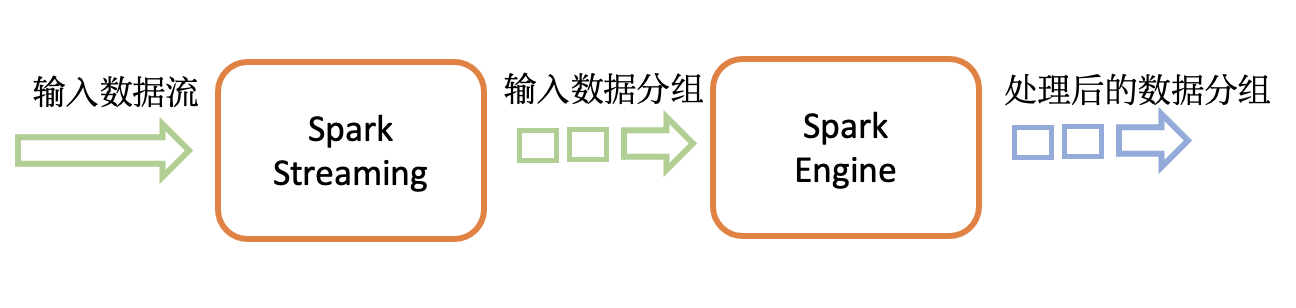
\includegraphics[scale=0.6]{spark工作原理.png}
    % 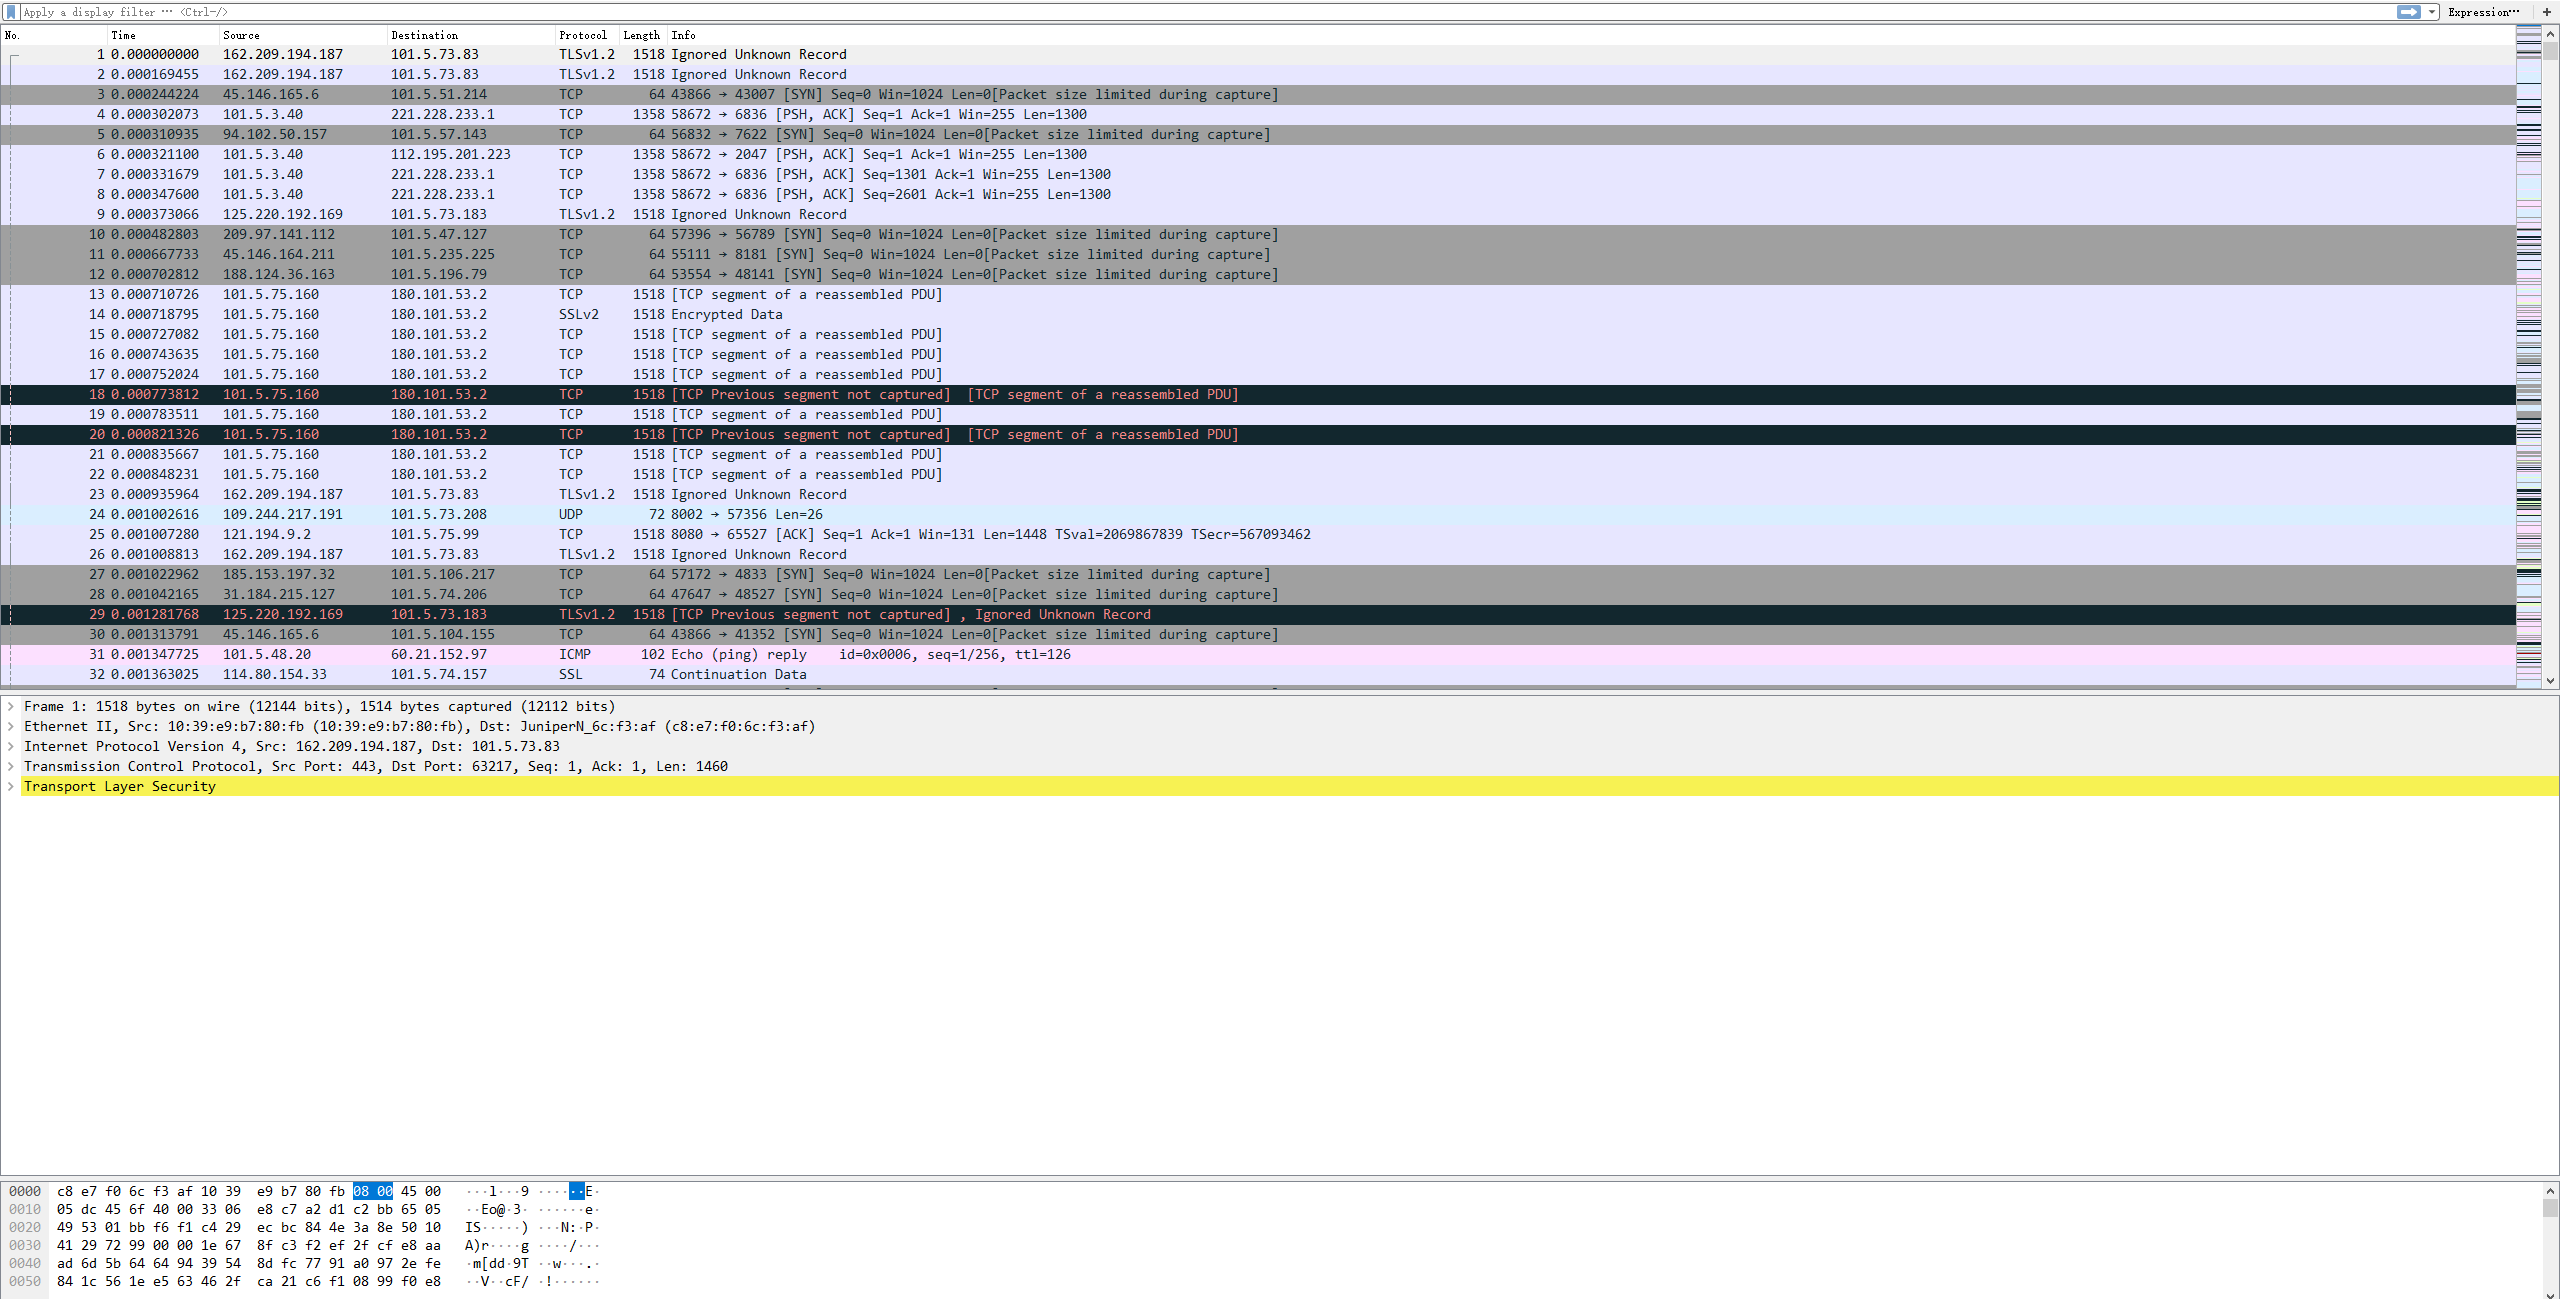
\includegraphics[width=0.6\linewidth]{wireshark流量图.png}
    \caption{spark工作原理}
    \label{fig:spark工作原理}
  \end{figure}

DStream是Spark Streaming中对数据流的一个抽象。DStream以哈希表的方式保存一
系列连续的RDD,哈希表的键是时间,值是RDD。随着时间的推移,DStream中产生新
的RDD,形成一个RDD流,但是由于RDD还是批处理方式,而且往往RDD中的数据量相
对较小,所以SparkStreaming对于数据的处理又称为微批处理。此外DStream和RDD—样,
提供map、foreach、flatMap、transform等算子。

Spark Streaming支持基本数据源和高级数据源,其中基本数据源包括hdfs(hadoop File System)文件源,简单socket源等,高级数据源包括kafka,Flume等。Spark Streaming
在执行的过程可以分成两个阶段,数据准备阶段和数据计算阶段,以下分别介绍。

下图~\ref{fig:spark}展示Spark Streaming接收数据的示意图,其中BlockGenerator,Receiver都是
Spark Streaming实现的组件,blockForPushing是一个阻塞队列。在Spark Streaming数
据准备阶段,首先Receiver从外部数据源接收数据并且将数据写入BlockGenerator的
ArrayBuffer(内存数组)中,该过程会保证数据接收速率始终小于设置的最大速率
maxRate,这个maxRate也可以由Spark的反压模块根据Spark集群的处理速度自行计算。
然后,BlockGenerator包含定时器Timer会定时将ArrayBuffer中的数据生成Block对象(块
对象,其中包含生成的数据),并且将Block对象写入BlockForPushing阻塞队列中,然后
再通知SparkStreaming的Driver程序,将Block对象分配至Block队列。最终,数据在Block
队列中等待Spark Streaming的计算阶段。以上便是Spark Streaming接收数据的全部过程。
\begin{figure}
    \centering
    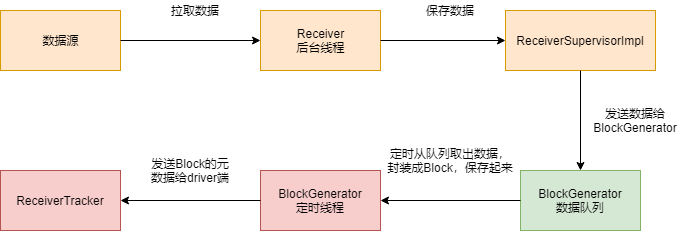
\includegraphics[scale=0.6]{spark数据源.png}
    \caption{Spark数据源}
    \label{fig:spark}
  \end{figure}

  下图~\ref{fig:spark streaming}是Spark Streaming作业的执行流程,具体流程分为以下几步:
  \begin{figure}
    \centering
    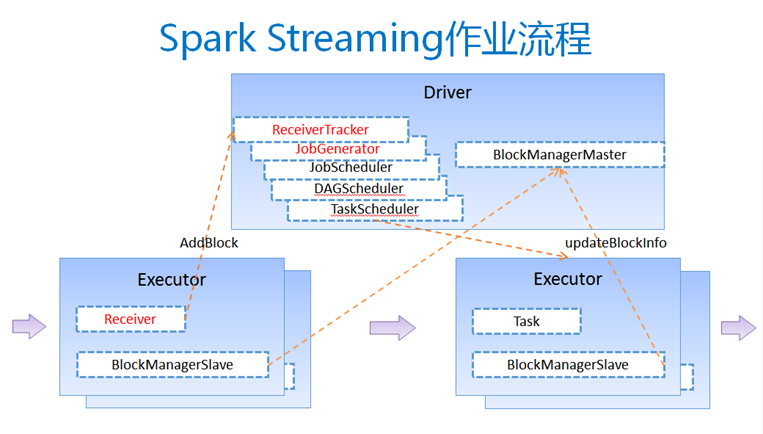
\includegraphics[scale=0.6]{spark执行流程.png}
    \caption{spark streaming执行流程}
    \label{fig:spark streaming}
  \end{figure}
 
  \begin{enumerate}[1.]
      \item  客户端提交作业后启动Driver,Driver是park作业的Master。
      \item 每个作业包含多个Executor,每个Executor以线程的方式运行task,Spark Streaming至少包含一个receiver task。
      \item Receiver接收数据后生成Block,并把BlockId汇报给Driver,然后备份到另外一个Executor上。
      \item ReceiverTracker维护Reciver汇报的BlockId。
      \item Driver定时启动JobGenerator,根据Dstream的关系生成逻辑RDD,然后创建Jobset,交给JobScheduler。
      \item JobScheduler负责调度Jobset,交给DAGScheduler,DAGScheduler根据逻辑RDD,生成相应的Stages,每个stage包含一到多个task。
      \item TaskScheduler负责把task调度到Executor上,并维护task的运行状态。
      \item 当tasks,stages,jobset完成后,单个batch才算完成。
  \end{enumerate}

\section{流式数据特征抽取}
Spark Streaming 支持 Scala、Java 和 Python,本文中使用Python提交任务。使用第三章中的特征提取方法,
输入为由kafka传入的流量数据,提取的结果都是传输层的一些统计信息,以一个TCP流或一个UDP流为一个单位。TCP流以FIN标志为结束,UDP以设置的flowtimeout时间为限制,超过时间就判为结束。在一个TCP流中有很多个数据包,先三次握手而后传输信息再四次挥手。统计一个流中的统计信息作为提取的特征。且统计的特征都分前后向,规定由源地址到目的地址为正向,目的地址到源地址为反向,为每个流构建一个标志叫Flow ID:192.168.31.100-183.232.231.174-46927-443-6,由源地址、目的地址、协议号组成。
流量特征提取的整体流程图如下:
TODO:修改图片!
\begin{figure}
    \centering
    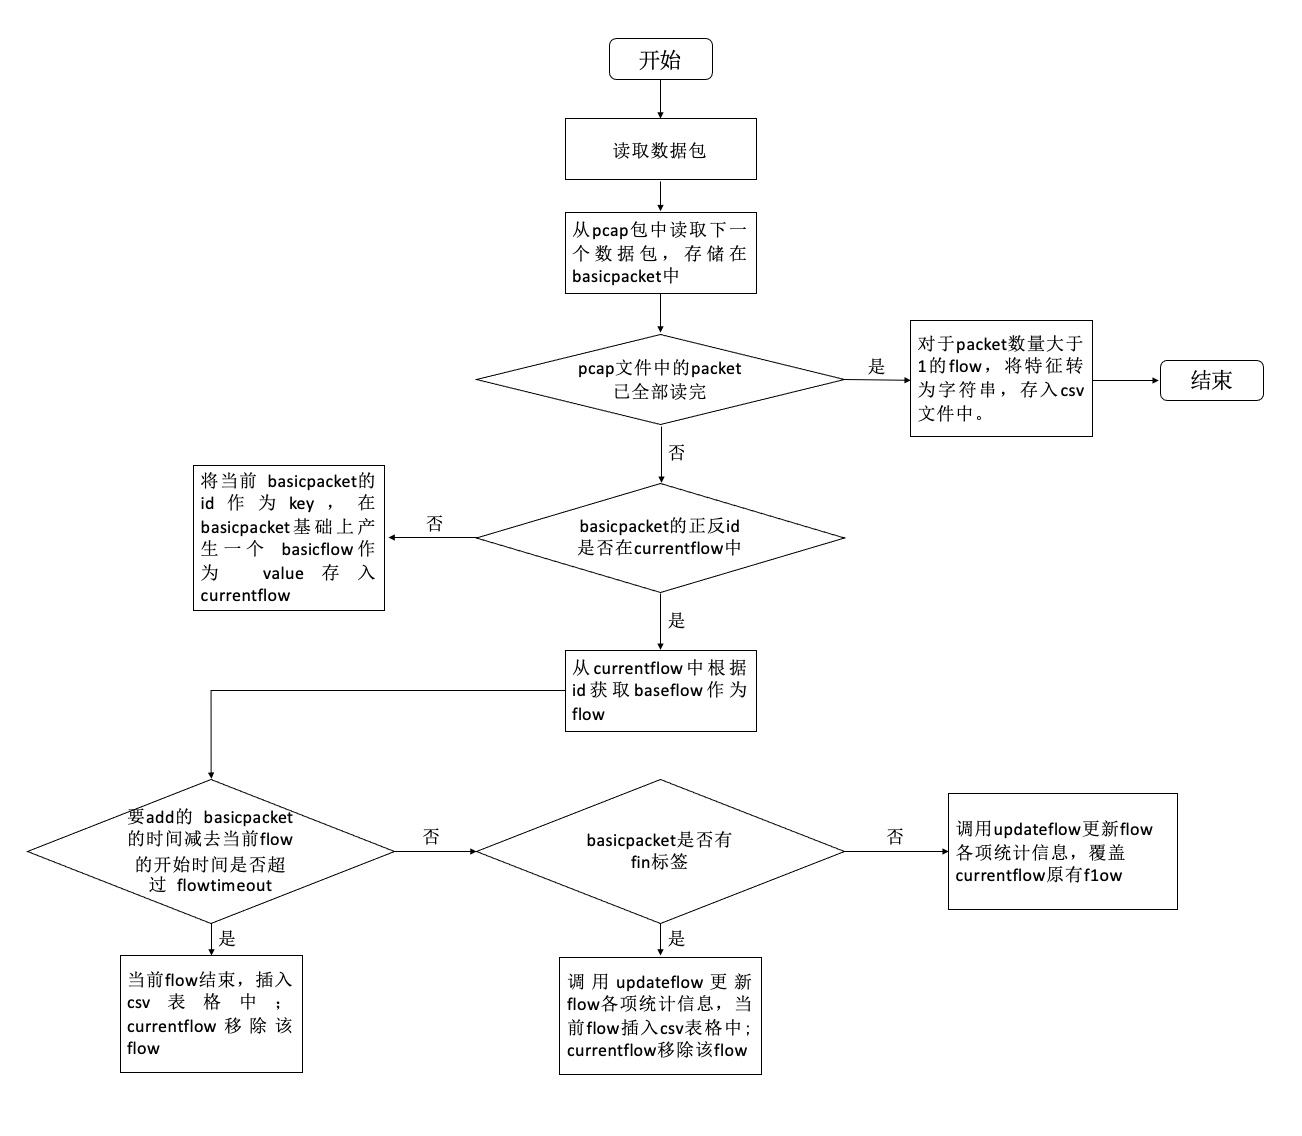
\includegraphics[scale=0.2]{特征提取.jpg}
    \caption{特征提取}
    \label{fig:特征提取}
  \end{figure}

从pcap文件中逐个读取packet,将每个数据包添加到对应的流中在currentFlows存储当前还未结束得所有TCP、UDP流。在添加的过程中不断地更新每个流的统计特征,最终将统计特征写入csv文件。判断新加入的数据包是否属于当前所有未结束的流,如果属于当前流则判断正向还是反向,之后判断时间是否超时、不超时则判断是否含有FIN标志,如果两者都不满足,则声明一个BasicFlow对象,根据id从currentFlows中拿到与当前数据包对应的流,调用addPacket将该数据包加入到对应流中。如果前面判断不在当前所有未结束的流中,则直接创建一个新得流,里面只含当前数据包,存入到currentFlows中。如果属于当前某个未结束的流,且超时或存在FIN标志,则说明当前flow结束,超时则从currentFlows中移除对应流,新建flow存入currentFlows中,含FIN标志则直接从currentFlows中移除对应流。结束的flow直接调用onFlowGenerated函数将流打印存储起来。

使用该方法得到的csv文件如下所示:
\begin{figure}
    \centering
    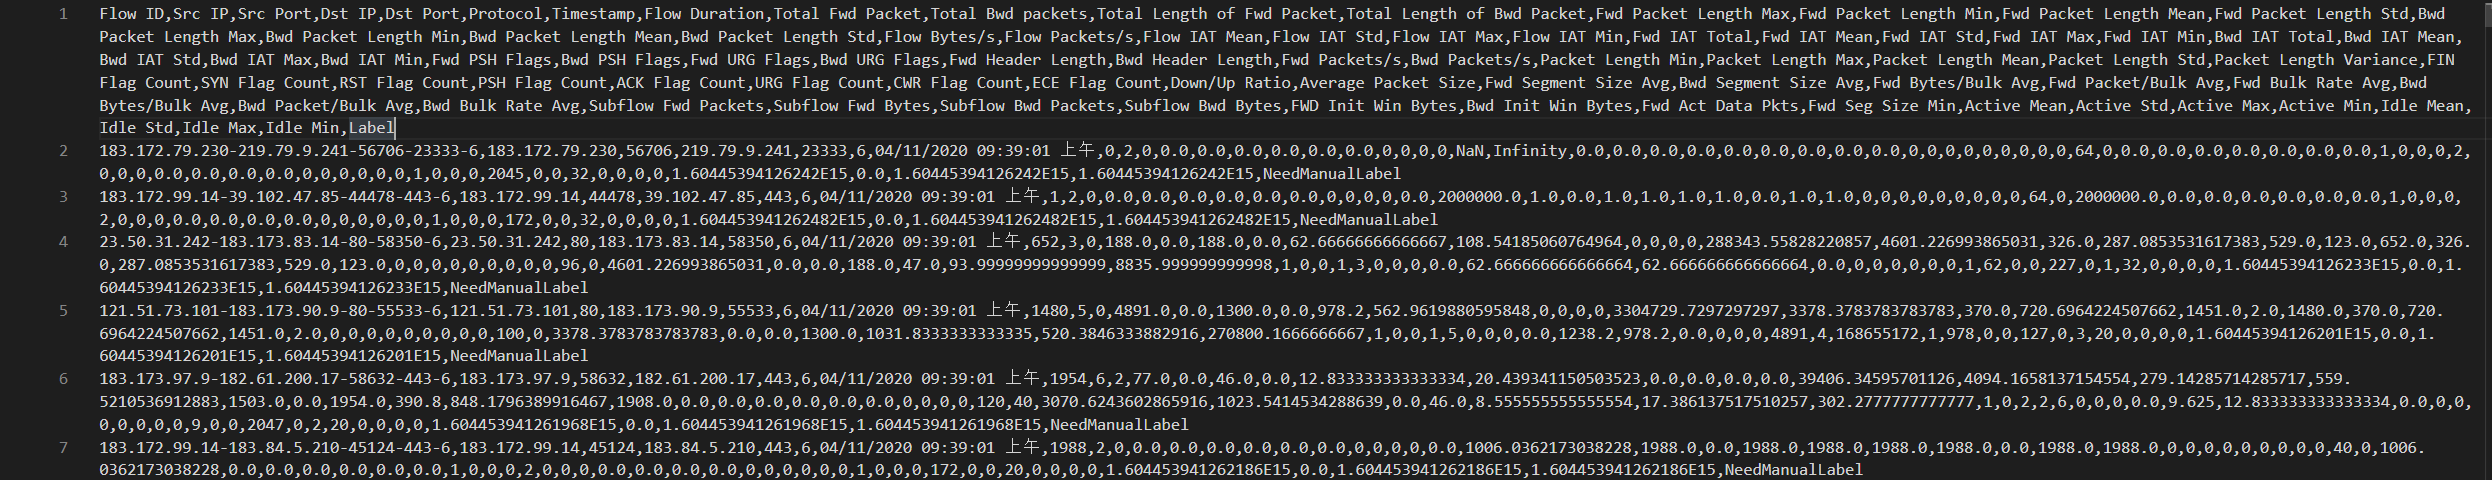
\includegraphics[scale=0.2]{特征文件.png}
    \caption{特征文件}
    \label{fig:特征文件}
  \end{figure}


\section{模型训练模块的设计与实现}
补充一些图
\section{预测输出模块}
\section{系统结果展示与分析}
本章在第二章技术分析和介绍的基础上,先后阐述异常流量检测系统的需求分析、
本文系统总体架构的设计、算法模型的设计方案,最后根据系统的总系架构和算法模型
提出本文系统五大模块的设计方案。
3.1需求分析
3.1.1功能需求分析
根据项目背景,本文设计的系统功能需求为:
(1)能够通过JnetPcap技术采集主机流量特征,采集pcap类型文件中的保存的流量特
征。
(2)能够将采集端的采集特征在后台收集端集中,过滤,写入kafka。
(3)能够对流量预测,本文将流量分成4等级,等级越高,是异常流量的可能性越大。
(4)能够对预测的结果进行良好的展示。
(5)预测模型具有一定效果。
3.1.2系统需求分析
(1)可扩展:随着后期需求的变化与增长,所以在开发过程需要考虑如何应付这些后
期变化。针对本系统,需要考虑采集模块支持Windows、Linux系统,需要考虑预测模块
中模型的更新和替换问题。
(2)健壮性:在流式处理的过程中,有可能其中一个模块偶尔发生错误,不能让这种
错误影响到整体系统运行,但是需要对这种错误进行记录。
(3)配置分离:系统的某些属性需要以配置文件的形式分离出来,方便以后对系统的
管理控制。
3.2系统总体设计
3.2.1异常流量预测系统总体架构设计
本系统属于流式系统,采集模块获取数据包流量的特征,并且实时对流量进行预测,
最后以报表的形式展示出来。结合需求和相关技术的分析,本文系统总体设计如图所
示,下面分别对各个模块的功能进行介绍。

3.2.2异常流量预测系统运行流程简介
在系统环境已经部署好的情况下,结合异常流量的总体架构设计,该系统运行的整
体流程如图3-2所示,图中编号代表这个模块运行的步骤。
% (1)训练离线模型。离线模型训练需要脱离整个数据流运行,本系统主要具有两个模
% 型,分另丨J是KMeans
% _
% RandomForest
% _
% Model和Streaming
% _
% KJVleans
% _
% Model,其中
% KMeans
% _
% RandomForest
% _
% Model基于K-Means算法和RandomForest算法实现,是监督模
% 型,需要标注数据,预测效果好;Streaming
% +
% KMeans
% +
% Modd是无监督的机器学习模型,
% 18
% 不需要标注数据,但是需要提供初始化参数,该模型预测效果不如
% KMeans
% —
% RandomForest
% —
% Model〇
(2)开启后台收集模块,收集端应该先于采集端运行,不然会导致采集端发送的数据
丢失。
(3)开启采集模块,采集并发送数据。
(4)向Spark集群提交预测模块任务,从kafka中源源不断的读取数据,并且将预测后
的结果写入一个新的kafka topic。
(4)开启报表模块展示预测结果。





% 其他部分
\backmatter

% 参考文献
\bibliography{ref/refs}  % 参考文献使用 BibTeX 编译
% \printbibliography       % 参考文献使用 BibLaTeX 编译

% 附录
\appendix
\chapter{补充内容}

附录是与论文内容密切相关、但编入正文又影响整篇论文编排的条理和逻辑性的资料,例如某些重要的数据表格、计算程序、统计表等,是论文主体的补充内容,可根据需要设置。


\section{图表示例}

\subsection{图}

附录中的图片示例(图~\ref{fig:appendix-figure})。

\begin{figure}
  \centering
  
\includegraphics[width=0.6\linewidth]{example-image-a.pdf}
  \caption{附录中的图片示例}
  \label{fig:appendix-figure}
\end{figure}


\subsection{表格}

附录中的表格示例(表~\ref{tab:appendix-table})。

\begin{table}
  \centering
  \caption{附录中的表格示例}
  \begin{tabular}{ll}
    \toprule
    文件名          & 描述                         \\
    \midrule
    thuthesis.dtx   & 模板的源文件,包括文档和注释 \\
    thuthesis.cls   & 模板文件                     \\
    thuthesis-*.bst & BibTeX 参考文献表样式文件    \\
    thuthesis-*.bbx & BibLaTeX 参考文献表样式文件  \\
    thuthesis-*.cbx & BibLaTeX 引用样式文件        \\
    \bottomrule
  \end{tabular}
  \label{tab:appendix-table}
\end{table}


\section{数学公式}

附录中的数学公式示例(公式~\eqref{eq:appendix-equation})。
\begin{equation}
  \frac{1}{2 \symup{\pi} \symup{i}} \int_\gamma f = \sum_{k=1}^m n(\gamma; a_k) \mathscr{R}(f; a_k)
  \label{eq:appendix-equation}
\end{equation}

% % !TeX root = ../thuthesis-example.tex

\begin{survey}
\label{cha:survey}

\title{Title of the Survey}
\maketitle


\tableofcontents


本科生的外文资料调研阅读报告。


\section{Figures and Tables}

\subsection{Figures}

An example figure in appendix (Figure~\ref{fig:appendix-survey-figure}).

\begin{figure}
  \centering
  
\includegraphics[width=0.6\linewidth]{example-image-a.pdf}
  \caption{Example figure in appendix}
  \label{fig:appendix-survey-figure}
\end{figure}


\subsection{Tables}

An example table in appendix (Table~\ref{tab:appendix-survey-table}).

\begin{table}
  \centering
  \caption{Example table in appendix}
  \begin{tabular}{ll}
    \toprule
    File name       & Description                                         \\
    \midrule
    thuthesis.dtx   & The source file including documentaion and comments \\
    thuthesis.cls   & The template file                                   \\
    thuthesis-*.bst & BibTeX styles                                       \\
    thuthesis-*.bbx & BibLaTeX styles for bibliographies                  \\
    thuthesis-*.cbx & BibLaTeX styles for citations                       \\
    \bottomrule
  \end{tabular}
  \label{tab:appendix-survey-table}
\end{table}


\section{Equations}

An example equation in appendix (Equation~\eqref{eq:appendix-survey-equation}).
\begin{equation}
  \frac{1}{2 \symup{\pi} \symup{i}} \int_\gamma f = \sum_{k=1}^m n(\gamma; a_k) \mathscr{R}(f; a_k)
  \label{eq:appendix-survey-equation}
\end{equation}


\section{Citations}

Example citations in appendix.
\cite{abrahams99tex}
\cite{salomon1995advanced}
\cite{abrahams99tex,salomon1995advanced}


\bibliographystyle{unsrtnat}
\bibliography{ref/appendix}

\end{survey}
       % 本科生:外文资料的调研阅读报告
% % !TeX root = ../thuthesis-example.tex

\begin{translation}
\label{cha:translation}

\title{书面翻译题目}
\maketitle

\tableofcontents


本科生的外文资料书面翻译。


\section{图表示例}

\subsection{图}

附录中的图片示例(图~\ref{fig:appendix-translation-figure})。

\begin{figure}
  \centering
  
\includegraphics[width=0.6\linewidth]{example-image-a.pdf}
  \caption{附录中的图片示例}
  \label{fig:appendix-translation-figure}
\end{figure}


\subsection{表格}

附录中的表格示例(表~\ref{tab:appendix-translation-table})。

\begin{table}
  \centering
  \caption{附录中的表格示例}
  \begin{tabular}{ll}
    \toprule
    文件名          & 描述                         \\
    \midrule
    thuthesis.dtx   & 模板的源文件,包括文档和注释 \\
    thuthesis.cls   & 模板文件                     \\
    thuthesis-*.bst & BibTeX 参考文献表样式文件    \\
    thuthesis-*.bbx & BibLaTeX 参考文献表样式文件  \\
    thuthesis-*.cbx & BibLaTeX 引用样式文件        \\
    \bottomrule
  \end{tabular}
  \label{tab:appendix-translation-table}
\end{table}


\section{数学公式}

附录中的数学公式示例(公式~\eqref{eq:appendix-translation-equation})。
\begin{equation}
  \frac{1}{2 \symup{\pi} \symup{i}} \int_\gamma f = \sum_{k=1}^m n(\gamma; a_k) \mathscr{R}(f; a_k)
  \label{eq:appendix-translation-equation}
\end{equation}


\section{文献引用}

文献引用示例\cite{abrahams99tex}。


% 书面翻译的参考文献
\bibliographystyle{unsrtnat}
\bibliography{ref/appendix}

% 书面翻译对应的原文索引
\begin{translation-index}
  \nocite{salomon1995advanced}
  \bibliographystyle{unsrtnat}
  \bibliography{ref/appendix}
\end{translation-index}

\end{translation}
  % 本科生:外文资料的书面翻译

% 致谢
% !TeX root = ../thuthesis-example.tex

\begin{acknowledgements}
  衷心感谢我的导师李风华老师,他对我的教导如春风般温暖,同时又催人上进,李老师不仅在学术上给予我详细的指导,在我面对困难颓废退缩时给我指明方向,鼓励我坚持前行。

  感谢课题组的其他老师,为我提供丰富的科研资源、开放的科研环境,使我开阔了眼界,增长了能力。

  感谢实验室的荣成浩、庄淑颖、陈昕、徐超、沈钲晨等同学,我从和他们日常的讨论中获益良多,很多idea都迸发在激烈的探讨中。同时感谢宋兆杰、于淼、赵正品、蓝天鸣、李果等同学,很荣幸和你们一起度过三年的研究生生涯。

  % 衷心感谢导师×××教授和物理系××副教授对本人的精心指导。他们的言传身教将使我终生受益。

  % 在美国麻省理工学院化学系进行九个月的合作研究期间,承蒙 Robert Field 教授热心指导与帮助,不胜感激。

  % 感谢×××××实验室主任×××教授,以及实验室全体老师和同窗们学的热情帮助和支持!

  % 本课题承蒙国家自然科学基金资助,特此致谢。
\end{acknowledgements}


% 声明
\statement
% 生成的声明页是否要插入页眉和页脚(默认 empty)
% 仅在需要进行电子签名时,才需要打开这一选项
% 插入的扫描声明页总是会生成页眉(研究生)和页脚,不受这一选项影响
% \statement[page-style=plain]
% 将签字扫描后的声明文件 scan-statement.pdf 替换原始页面
% \statement[file=scan-statement.pdf]

% 个人简历、在学期间完成的相关学术成果
% !TeX root = ../thuthesis-example.tex

\begin{resume}

  \section*{个人简历}

  1993 年 5 月 20 日出生于河北省定州市。

  2011 年 9 月考入吉林大学机械科学与工程学院机械工程及自动化专业,2015 年 7 月本科毕业并获得工学学士学位。

  2018 年 9 月考入清华大学网络研究院攻读网络空间安全专业硕士至今。


  \section*{在学期间完成的相关学术成果}

  \subsection*{学术论文}

  \begin{achievements}
    \item Gao T, Li F, Yuan Q, et al. A New Factor Affecting the Performance of Wireless Networks: Port Scan[C]//2021 17th International Wireless Communications \& Wireless Networks Conference (IWCMC).(已被IWCMC录用,EI收录)
    \item Wang H, Gao T, et al.Hopping on Spectrum: Measuring and Boosting a Large-scale Dual-band Wireless Network[J]//USENIX ATC '21.(在投)
  \end{achievements}


  % \subsection*{专利}

  % \begin{achievements}
  %   \item 任天令, 杨轶, 朱一平, 等. 硅基铁电微声学传感器畴极化区域控制和电极连接的方法: 中国, CN1602118A[P]. 2005-03-30.
  %   \item Ren T L, Yang Y, Zhu Y P, et al. Piezoelectric micro acoustic sensor based on ferroelectric materials: USA, No.11/215, 102[P]. (美国发明专利申请号.)
  % \end{achievements}

\end{resume}


% 指导教师/指导小组学术评语
% !TeX root = ../thuthesis-example.tex

\chapter{指导小组学术评语}

论文提出了……


% 答辩委员会决议书
% !TeX root = ../thuthesis-example.tex

\chapter{答辩委员会决议书}

论文提出了……

论文取得的主要创新性成果包括:

1. ……

2. ……

3. ……

论文工作表明作者在×××××具有×××××知识,具有××××能力,论文××××,答辩××××。

答辩委员会表决,(×票/一致)同意通过论文答辩,并建议授予×××(姓名)×××(门类)学博士/硕士学位。


% 本科生的综合论文训练记录表(扫描版)
% \record{file=scan-record.pdf}

\end{document}
